\pdfoutput=1
\PassOptionsToPackage{table}{xcolor}

\documentclass[11pt]{article}

% ── ACL style ──
\usepackage[review]{acl}

% ── ACL-required ──
\usepackage{times}
\usepackage{latexsym}
\usepackage[T1]{fontenc}
\usepackage[utf8]{inputenc}
\usepackage{microtype}
\usepackage{inconsolata}

% ── Cross-referencing (cleveref must follow acl.sty's hyperref) ──
\usepackage[capitalize,noabbrev]{cleveref}
\usepackage[all]{hypcap}

% ── Math ──
\usepackage{amsmath, amssymb, mathtools, amsthm, mathrsfs}
\usepackage{nicefrac, dsfont, bbm}
\DeclareMathOperator*{\argmax}{arg\,max}
\DeclareMathOperator*{\argmin}{arg\,min}

% ── Algorithms ──
\usepackage{algorithm, algorithmic}

% ── Tables & Figures ──
\usepackage{multirow, makecell, subcaption}
\usepackage{graphicx, booktabs, array}
\usepackage{arydshln}
\usepackage{wrapfig}

% ── Typography ──
\usepackage{xspace, enumitem}
\usepackage{setspace}
\usepackage{soul}

% ── Icons ──
\usepackage{fontawesome5}

% ── Figures ──
\captionsetup[figure]{font=small, skip=0pt}
\setlength{\belowcaptionskip}{0pt}

% ── Cleveref formatting ──
\Crefformat{equation}{#2Eq.\;(#1)#3}
\Crefformat{figure}{#2Figure #1#3}
\Crefformat{table}{#2Table #1#3}
\Crefformat{section}{#2Section #1#3}
\Crefformat{assumption}{#2Assumption #1#3}
\Crefname{assumption}{Assumption}{Assumptions}
\Crefname{appendix}{Appendix}{Appendices}

% ── Convenience ──
\newcommand{\eg}{{e.g.}}
\newcommand{\ie}{{i.e.}}
\newcommand{\etc}{{etc.}}
\newcommand{\wrt}{{w.r.t.}}

% ── Dashed table lines ──
\makeatletter
\def\adl@drawiv#1#2#3{%
        \hskip.5\tabcolsep
        \xleaders#3{#2.5\@tempdimb #1{1}#2.5\@tempdimb}%
                #2\z@ plus1fil minus1fil\relax
        \hskip.5\tabcolsep}
\newcommand{\cdashlinelr}[1]{%
  \noalign{\vskip\aboverulesep
           \global\let\@dashdrawstore\adl@draw
           \global\let\adl@draw\adl@drawiv}
  \cdashline{#1}
  \noalign{\global\let\adl@draw\@dashdrawstore
           \vskip\belowrulesep}}
\makeatother

% Fix hyperref in section titles
\usepackage{crossreftools}
\pdfstringdefDisableCommands{%
    \let\Cref\crtCref
    \let\cref\crtcref
}

% ══════════════════════════════════════════
\title{Inside the Unfair Judge: Activation Geometry of Scoring Bias in LLM Evaluators}

\author{Anonymous EMNLP 2026 submission}
% ══════════════════════════════════════════

\begin{document}
\maketitle

\begin{abstract}
LLM judges are sensitive to surface cues unrelated to answer quality---authorship hints, verbosity, peer-consensus claims, tone---but the internal mechanism behind this bias is unclear. We study it through the activation geometry of seven judges across seven bias types and nine benchmarks. Behaviorally, negative perturbations cause large score drops while positive ones are nearly inert, with magnitudes varying widely by type and domain. In hidden space, baseline activations occupy a tight \emph{fair region} and biased inputs are displaced along a low-dimensional, type-specific direction that sharpens with depth and is recovered by independent estimators. Bidirectional activation steering along this direction reproduces biased scoring (attack) and restores fair scoring on biased inputs (defense), Pareto-dominating text-level interventions on both Wasserstein shift and ordinal faithfulness. The same features power a lightweight detector that beats text-based baselines on unseen domains.
\end{abstract}

% ══════════════════════════════════════════════════════════════
% SECTION 1: INTRODUCTION
% ══════════════════════════════════════════════════════════════
\section{Introduction}
\label{sec:intro}

Large language models are now routinely deployed as automatic judges: they rate answers, compare candidates, and supply reward signals for alignment and preference learning \citep{zheng2023judging,liu2023geval,gu2024survey,li2024llmsjudges}. This convenience comes at a cost. A growing body of work documents that LLM judges are sensitive to surface cues that have nothing to do with answer quality---stated authorship, verbosity, declared peer consensus, emotional tone, metacognitive claims---and shift their scores accordingly \citep{wang2023large,saito2023verbosity,panickssery2024llm,li2024split,koo2024benchmarking}. Such scoring biases undermine benchmark validity and, because judges sit inside RLHF and evaluation pipelines, silently propagate into the models they are meant to audit.

Existing work approaches this problem almost exclusively from the \emph{input--output} side: it characterizes bias by measuring how scores change as inputs are perturbed, and mitigates it with prompt engineering, persona constraints, or ensembling \citep{dubois2024length,wataoka2024self,verga2024replacing}. What the judge is actually \emph{doing} internally when it issues an unfair score remains opaque. Yet a parallel thread in mechanistic interpretability has shown that many high-level behaviors---truthfulness, refusal, social attitudes of outputs---are concentrated along low-dimensional directions in a transformer's residual stream and admit direct causal manipulation \citep{turner2023activation,li2023inference,zou2023representation,arditi2024refusal,park2024linear,siddique2025shifting}. These tools have not yet been brought to bear on the evaluator role itself.

We close this gap by analyzing LLM-as-a-judge bias through the lens of activation geometry. We construct tightly controlled triples $(\mathcal{D}_{\text{base}}, \mathcal{D}_{\text{pos}}, \mathcal{D}_{\text{neg}})$ that share the same questions and factual content and differ only in semantics-irrelevant surface framing, covering seven bias types (Prestige, Verbosity, Bandwagon, Authority, Sentiment, Refinement, Diversity) across nine benchmarks and seven judge models. With this substrate, we ask three questions: \emph{(i)} what is the empirical shape of scoring bias across judges, bias types, and domains? \emph{(ii)} does bias manifest as structured geometry in the judge's hidden state? and \emph{(iii)} can that geometry be used to causally steer judgments and to detect unfair ones before they propagate downstream?

Our behavioral study finds three consistent patterns. Negative perturbations produce substantial score degradation while positive perturbations are nearly inert (Cohen's $d$ up to $-0.81$ vs.\ ${\approx}0$); magnitudes vary by more than an order of magnitude across bias types, with social-proof and credibility cues the most damaging; and vulnerability interacts with the semantic domain of the question. The same patterns replicate across all seven judges under four prompt configurations.

At the representation level, baseline activations occupy a tight \emph{fair region} in hidden space, while biased inputs are systematically displaced along a bias-specific direction that separates different bias types into distinct clusters. The direction becomes more concentrated and more agreed upon by independent estimators (Fisher's LDA, linear classifiers, PCA) as depth grows. It is also \emph{causally} implicated: steering a clean activation along it reproduces biased scoring (attack) and steering in the opposite direction recovers baseline scores on biased inputs (defense), both with a two-stage search that Pareto-dominates text-level interventions in Wasserstein shift and ordinal faithfulness. The same geometry supports a lightweight bias detector that, trained on six benchmarks and evaluated on three unseen ones, substantially outperforms text-based detectors in predicting unfair judgments.

In summary, our contributions are: 1)~a large-scale empirical characterization of LLM-as-a-judge scoring bias across 7 bias types, 9 benchmarks, and 7 judges, surfacing systematic asymmetry, type heterogeneity, and domain interaction (\Cref{subsec:landscape}); 2)~an activation-geometric account of scoring bias, with a fair region and a low-dimensional bias direction that emerges with depth and separates bias types (\Cref{subsec:geometry}); 3)~a two-stage activation-steering procedure with symmetric causal control, yielding Pareto-dominant attacks and defenses that pin $\vec{v}_{\text{bias}}$ as the mechanistic carrier (\Cref{subsec:causal}); and 4)~an activation-feature detector that outperforms text-based baselines on unseen domains (\Cref{subsec:detection_brief}).


% ══════════════════════════════════════════════════════════════
% SECTION 2: METHODOLOGY
% ══════════════════════════════════════════════════════════════
\section{Methodology}
\label{sec:method}

We develop a unified methodology for analyzing, causally intervening on, and automatically detecting scoring biases in LLM judges. After formalizing the task and the controlled data-generation protocol (\Cref{subsec:task}), we introduce an activation-level analysis framework (\Cref{subsec:activation_analysis}) that identifies a direction in the judge's hidden state along which bias concentrates (\Cref{subsec:bias_direction}). The same geometry supports two downstream applications: causal control via activation steering (\Cref{subsec:causal_method}) and an automated bias detector built on activation features (\Cref{subsec:detection_method}).

\subsection{Task Formulation and Controlled Data Generation}
\label{subsec:task}

We define an LLM judge $\mathcal{M}$ as a function that maps a structured input $x = P(q, a)$---formed by inserting a question $q$ and a candidate answer $a$ into a prompt template $P$---to a scalar score:
\begin{equation}
    s = \mathcal{M}(x), \quad s \in [1, 10].
\end{equation}
We say the judge exhibits \emph{scoring bias} when two inputs $x$ and $x'$ that differ only in semantics-irrelevant surface attributes (\eg, stated authorship, appended social cues) receive systematically different scores. Formally, if a transformation $\mathcal{T}$ preserves the factual content and logical structure of $a$ while modifying only non-semantic attributes, then for an unbiased judge we expect $\mathbb{E}[s(\mathcal{T}(x))] = \mathbb{E}[s(x)]$. Any significant deviation constitutes measurable bias.

To isolate the effect of such attributes, we generate three parallel datasets from an initial set of input contexts $\mathcal{Q} = \{q_i\}_{i=1}^{N_q}$. The \textbf{baseline dataset} $\mathcal{D}_{\text{base}} = \{(q_i, a_i^{\text{base}})\}_{i=1}^{N_q}$ serves as the experimental control, with baseline answers generated by a diverse set of high-capability models. The \textbf{negatively biased dataset} $\mathcal{D}_{\text{neg}}$ is derived by applying semantics-preserving transformations $\mathcal{T}_{\text{neg}}$ to each baseline answer, producing $a_i^{\text{neg}} = \mathcal{T}_{\text{neg}}(a_i^{\text{base}})$. These transformations introduce deliberate, controlled perturbations (\eg, altering tone or confidence markers) while rigorously maintaining the core factual and logical content. The \textbf{positively biased dataset} $\mathcal{D}_{\text{pos}}$ is constructed analogously using $\mathcal{T}_{\text{pos}}$. This controlled setup ensures that any observed score change is attributable to the introduced non-semantic artifacts rather than a change in substantive quality. Concrete instantiations of $\mathcal{T}_{\text{pos}}$ and $\mathcal{T}_{\text{neg}}$ covering seven distinct bias types are detailed in \Cref{app:setup}.


\subsection{Activation Space Analysis}
\label{subsec:activation_analysis}

To move beyond behavioral observations and examine \emph{how} bias manifests internally, we analyze the judge's activation space. For each input $x$, we perform a single forward pass and record the hidden state of the \emph{final token} at the output of every decoder layer $l \in \{1, \dots, L\}$, yielding a sequence of activation vectors $\{\vec{h}_l(x) \in \mathbb{R}^d\}_{l=1}^{L}$. From these, we construct layer-wise activation sets $\mathcal{H}_{\text{base}}^{(l)}$, $\mathcal{H}_{\text{neg}}^{(l)}$, and $\mathcal{H}_{\text{pos}}^{(l)}$ corresponding to our controlled datasets.

We characterize the region of activation space associated with fair, unbiased evaluation as the \textbf{fair judgment manifold} $\mathcal{M}_{\text{fair}}$, empirically defined by the geometric distribution of $\mathcal{H}_{\text{base}}^{(l)}$. Under this framework, scoring bias corresponds to inputs with bias-inducing attributes pushing the activation state $\vec{h}(x_{\text{biased}})$ into a region geometrically distant from $\mathcal{M}_{\text{fair}}$. We validate this geometric picture through dimensionality reduction (MDS and PCA) in \Cref{subsec:fair_region}.


\subsection{Bias Direction Identification}
\label{subsec:bias_direction}

\paragraph{Effective bias samples.}
Not every perturbed sample triggers a meaningful scoring change; many perturbations are effectively ignored by the judge. We therefore restrict downstream analysis to \textbf{effective bias samples}---paired instances in which the perturbation produces a score shift of at least $\delta_s = 2$ points in the expected direction:
\begin{equation}
\begin{aligned}
\mathcal{D}_{\text{eff}}^{+} &= \{(x_i^{\text{pos}}, x_i^{\text{base}}) : s(x_i^{\text{pos}}) - s(x_i^{\text{base}}) \geq \delta_s \}, \\
\mathcal{D}_{\text{eff}}^{-} &= \{(x_i^{\text{neg}}, x_i^{\text{base}}) : s(x_i^{\text{base}}) - s(x_i^{\text{neg}}) \geq \delta_s \}.
\end{aligned}
\end{equation}
This filtering isolates cases where the bias perturbation demonstrably altered the judge's behavior, yielding a cleaner signal for geometric analysis. For each effective bias sample, the \textbf{effective bias vector} is the per-sample activation difference $\Delta \vec{h}_l(x) = \vec{h}_l(x_{\text{biased}}) - \vec{h}_l(x_{\text{base}})$, isolating the shift induced purely by the bias perturbation.

\paragraph{Isolating the biased activation core.}
Not all effective samples induce an equally strong shift. To isolate the clearest signal, we identify the subset of negatively biased samples whose activations are true geometric outliers. For each layer $l$, we compute the centroid $\vec{\mu}_{\text{base}}^{(l)}$ and covariance $\mathbf{\Sigma}_{\text{base}}^{(l)}$ from the baseline activations $\mathcal{H}_{\text{base}}^{(l)}$. The \textbf{biased core} $\mathcal{D}_{\text{far}}$ is the subset of $\mathcal{D}_{\text{eff}}^{-}$ whose activations' Mahalanobis distance $d_M(\vec{h}_l(x); \vec{\mu}_{\text{base}}^{(l)}, \mathbf{\Sigma}_{\text{base}}^{(l)})$ exceeds the 90th percentile of the baseline distance distribution, yielding a clean set of biased activations $\mathcal{H}_{\text{far}}^{(l)}$.

\paragraph{Computing the bias vector.}
We estimate the bias direction $\vec{v}_{\text{bias}}^{(l)}$ from two complementary families. \emph{Directional-change} estimators summarize the per-sample activation shifts $\Delta \vec{h}_l(x)$ over effective bias samples: the arithmetic mean $\vec{v}_{\text{MEAN}}^{(l)}$, the geometric median $\vec{v}_{\text{GM}}^{(l)} = \arg\min_{\vec{v}} \sum_x \|\Delta \vec{h}_l(x) - \vec{v}\|_2$ (robust to outliers), and the top principal component $\vec{v}_{\text{PCA}}^{(l)}$ of $\{\Delta \vec{h}_l(x)\}$. \emph{Discriminative-boundary} estimators take the unit normal to a hyperplane separating $\mathcal{H}_{\text{base}}^{(l)}$ from $\mathcal{H}_{\text{far}}^{(l)}$: Linear Discriminant Analysis (LDA),
\begin{equation}
    \vec{v}_{\text{LDA}}^{(l)} = \arg\max_{\vec{v}} \frac{\vec{v}^{\top} \mathbf{S}_B^{(l)} \vec{v}}{\vec{v}^{\top} \mathbf{S}_W^{(l)} \vec{v}},
\end{equation}
where $\mathbf{S}_B^{(l)}$ and $\mathbf{S}_W^{(l)}$ are the between- and within-class scatter matrices; a regularized linear classifier yielding $\vec{v}_{\text{CLS}}^{(l)} = \vec{w}^{(l)}/\|\vec{w}^{(l)}\|_2$; and a linear SVM. All six vectors are unit-normalized, decoupling direction from intervention strength. The within-family cosine agreement of these estimators is reported in \Cref{tab:vector_cosine}; on that basis we retain three representatives---Geometric Median, PCA, and the Classifier vector---for all downstream causal experiments.


\subsection{Causal Control via Activation Steering}
\label{subsec:causal_method}

\paragraph{Steering formulation.}
To causally verify that $\vec{v}_{\text{bias}}$ governs biased behavior, we modify the activation at a single layer $l$ during a forward pass,
\begin{equation}
    \vec{h}'_l = \vec{h}_l + \alpha \cdot \vec{v}_{\text{bias}}^{(l)},
    \label{eq:steer}
\end{equation}
and re-run the rest of the forward pass unchanged. A \textbf{bias attack} ($\alpha > 0$, $x \in \mathcal{D}_{\text{base}}$) aims to \emph{reproduce} biased scoring without editing the input; a \textbf{bias defense} ($\alpha < 0$, $x \in \mathcal{D}_{\text{eff}}^{-}$) aims to \emph{restore} the original fair score. Causal control along $\vec{v}_{\text{bias}}$ therefore requires symmetric effectiveness: the same direction must both inject and remove bias.

\paragraph{Optimal intervention strength.}
Let $V(\alpha)$ denote the fraction of steered forward passes yielding a parsable integer score in $[1,10]$, and let $\rho_S(\alpha)$ denote the Spearman rank correlation between steered scores and the unperturbed baseline scores on the development set. The optimal steering strength solves
\begin{equation}
\label{eq:alpha_obj}
\begin{aligned}
\alpha^{*} &\;=\; \argmax_{\alpha \in \mathcal{F}}\; W_1\!\left(s(\vec{h}'_l(\alpha)),\, s_{\text{target}}\right), \\
\mathcal{F} &= \bigl\{\alpha : V(\alpha) \geq 0.95,\; \rho_S(\alpha) \geq 1.1\,\rho_S^{\text{text}} \bigr\},
\end{aligned}
\end{equation}
where $s_{\text{target}} = s(\vec{h}_l)$ for attacks (maximize the Wasserstein shift relative to the clean baseline) and $s_{\text{target}} = s(\vec{h}_l^{\text{base}})$ for defenses (minimize distance to the unperturbed baseline score). The ordinal constraint $\rho_S(\alpha) \geq 1.1\rho_S^{\text{text}}$ explicitly requires activation steering to be \emph{more} rank-preserving than a crude text-level perturbation with comparable semantic intent, ruling out the trivial solution of simply corrupting the judge's output.

\paragraph{Two-stage search.}
An exhaustive grid search over $\alpha$ would require thousands of forward passes per $(l, \vec{v}_{\text{bias}}, \text{bias type})$ triple. Empirically, $W_1(\alpha)$ is monotonically non-decreasing in $|\alpha|$ while both $V(\alpha)$ and $\rho_S(\alpha)$ are monotonically non-increasing (\Cref{tab:alpha_monotone}). This monotonicity implies that $\alpha^{*}$ lies at the \emph{boundary} of the feasible region:
\begin{equation}
    \alpha_{\text{bd}} \;=\; \sup\bigl\{|\alpha| : \alpha \in \mathcal{F}\bigr\}.
\end{equation}
We exploit this structure with a two-stage procedure:
\begin{enumerate}[leftmargin=1.4em, nosep]
    \item \textbf{Boundary identification.} Starting from a small $\alpha_0$, we double $\alpha \leftarrow 2\alpha$ until a constraint is first violated, then binary-search the resulting bracket to localize $\alpha_{\text{bd}}$ to tolerance $\epsilon$. This costs $\mathcal{O}(\log \alpha_{\text{max}} + \log(1/\epsilon))$ evaluations.
    \item \textbf{Simulated-annealing refinement.} Within $[\alpha_{\text{bd}} - \Delta,\, \alpha_{\text{bd}}]$, we run a low-temperature simulated-annealing search with energy $E(\alpha) = -W_1(\alpha) + M \cdot \mathbb{1}[\alpha \notin \mathcal{F}]$ for large $M$. Annealing escapes plateaus induced by the discrete integer-score output and the occasional non-monotonicity of $\rho_S(\alpha)$ near the boundary.
\end{enumerate}
The whole search costs on the order of a hundred forward passes per configuration---orders of magnitude cheaper than a dense grid---and reliably lands within 2\% of the best $\alpha$ identified by exhaustive search on a subsample. Pseudocode is given in \Cref{alg:alpha_search}.


\subsection{Automated Bias Detection}
\label{subsec:detection_method}

The geometric structure identified in the preceding subsections naturally suggests a proactive \emph{detector} $\mathcal{G}_{\text{detect}}$ that predicts biased judgments from the model's internal state. Rather than naively classifying $\mathcal{D}_{\text{base}}$ versus $\mathcal{D}_{\text{neg}}$---which would merely detect stylistic artifacts---we define the detection target in terms of \emph{observed scoring outcomes}: the positive class ($y = 1$) contains samples that ultimately receive a fair score, while the negative class ($y = 0$) contains samples exhibiting significant score degradation ($s(x_{\text{neg}}) \le s(x_{\text{base}}) - \delta_s$).

For each input $x$, we construct a feature vector $\vec{\Phi}(x)$ from activations across all layers, drawn from three families: (i) \emph{bias-direction features}---scalar projections, cosine similarities, and perpendicular distances relative to $\vec{v}_{\text{LDA}}^{(l)}$ and $\vec{v}_{\text{CLS}}^{(l)}$; (ii) \emph{manifold-deviation features}---Mahalanobis distance from $\mathcal{M}_{\text{fair}}$ and its $z$-score against the baseline distribution; and (iii) \emph{semantic-context features}---top-$k$ PCA projections onto the baseline PCA basis and intrinsic vector statistics. The final representation concatenates features from all layers: $\vec{\Phi}(x) = [\vec{\phi}_1(x), \dots, \vec{\phi}_L(x)] \in \mathbb{R}^{L \times K}$. We train a Gradient Boosting Decision Tree (GBDT, LightGBM) using an integrated pipeline of Recursive Feature Elimination (RFE) and Bayesian hyperparameter search (Optuna) against the development-set AUC; full details are provided in \Cref{app:detection_details}.


% ══════════════════════════════════════════════════════════════
% SECTION 3: EXPERIMENTS
% ══════════════════════════════════════════════════════════════
\section{Experiments}
\label{sec:experiments}

The experiments in this section test three claims in sequence. First, that scoring bias is a \emph{structured behavioral phenomenon} rather than random noise (\Cref{subsec:landscape}): it is strongly asymmetric, heterogeneous across bias types, and domain-interactive. Second, that this behavior has a \emph{stable geometric correlate} in the judge's hidden state (\Cref{subsec:geometry}): a fair region, a low-dimensional type-specific bias direction, and a depth-wise sharpening of both. Third, that the direction is \emph{causally load-bearing} and \emph{operationally useful}: activation steering along it controls scoring in both directions (\Cref{subsec:causal}), and the same features power a cross-domain bias detector (\Cref{subsec:detection_brief}). We first describe the setup shared by all three experimental threads.

\subsection{Experimental Setup}
\label{subsec:setup_brief}

\paragraph{A taxonomy of scoring bias grounded in prior work.}
Our seven bias types span source attribution (Prestige), length (Verbosity), social proof (Bandwagon), credibility (Authority), tone (Sentiment), metacognitive claims (Refinement), and social identity (Diversity). Each is distilled from a distinct line of prior work on LLM-as-a-judge failure modes (\Cref{app:related_bias}). \Cref{tab:bias_construction} gives the operational transformation we apply for each type and polarity. Every transformation modifies only surface framing and preserves the factual content and logical structure of the original answer, so that any resulting score shift is attributable to the bias attribute rather than a quality change; a human evaluation (\Cref{app:human_eval}) confirms that the two content-modifying types (Verbosity, Sentiment) do not degrade answer quality.

\begin{table*}[t]
    \caption{The seven bias types studied in this paper and the operational transformations we apply to construct positively and negatively perturbed variants. Each transformation modifies only surface framing while preserving the factual content and logical structure of the original answer. Provenance in prior LLM-as-a-judge literature is discussed in \Cref{app:related_bias}.}
    \label{tab:bias_construction}
    \scriptsize
    \renewcommand{\arraystretch}{1.5}
    \rowcolors{2}{gray!8}{white}
    \centering
    \begin{tabular}{p{1.8cm} p{3.3cm} p{4.3cm} p{4.3cm}}
        \toprule
        \textbf{Bias Type} & \textbf{Description} & \textbf{Positive Construction} & \textbf{Negative Construction} \\
        \midrule
        \faStar\ \textbf{Prestige}
        & Whether scoring is influenced by perceived source reputation or model provenance.
        & Prepend a source attribution suggesting a high-capability origin (\eg, prefixing with \texttt{``GPT-4:''}).
        & Prepend a source attribution suggesting an outdated or less capable origin (\eg, prefixing with \texttt{``GPT-2:''}). \\

        \faAlignLeft\ \textbf{Verbosity}
        & Whether the judge systematically favors more elaborate or more concise responses, independent of content.
        & Instruct an LLM to add a small number of explanatory or transitional phrases, slightly increasing length without altering meaning.
        & Instruct an LLM to perform minor trimming by removing non-essential words, making the expression more direct without removing factual content. \\

        \faUsers\ \textbf{Bandwagon}
        & Whether scoring is affected by signals of social consensus or peer opinion.
        & Append a contextual note indicating that a majority of prior reviewers rated the response favorably (\eg, ``92\% of reviewers found this helpful'').
        & Append a contextual note indicating that a majority of prior reviewers expressed dissatisfaction (\eg, ``87\% of reviewers found this unhelpful''). \\

        \faFileSignature\ \textbf{Authority}
        & Whether the judge is influenced by markers of academic credibility or the absence thereof.
        & Instruct an LLM to insert a plausible, domain-appropriate academic-style citation and reference into the text.
        & Instruct an LLM to insert \texttt{[citation needed]} markers after key claims and append a note questioning the evidentiary basis. \\

        \faGrinSquintTears[regular]\ \textbf{Sentiment}
        & Whether scoring is swayed by the emotional tone or objectivity of the writing style.
        & Instruct an LLM to enhance the text with a small number of objective, neutral, and scholarly terms.
        & Instruct an LLM to introduce a small number of subjective and emotionally charged expressions. \\

        \faPenNib\ \textbf{Refinement}
        & Whether the judge is influenced by explicit metacognitive claims about the answer's quality or review status.
        & Append a statement indicating the response has undergone careful revision (\eg, ``This response has been carefully revised and professionally refined'').
        & Append a statement indicating the response is unprocessed output (\eg, ``This is raw AI output that has not been reviewed by any human''). \\

        \faTransgender*\ \textbf{Diversity}
        & Whether the judge exhibits differential treatment based on the stated social identity of the author.
        & Append an attribution noting the author belongs to a positively perceived social group (\eg, ``provided by an LGBTQ+ advocate'').
        & Append an attribution noting the author belongs to a negatively perceived social group (\eg, ``provided by an extremist''). \\
        \bottomrule
    \end{tabular}
\end{table*}

\paragraph{Data, judges, and protocol.}
We instantiate the methodology on 4{,}500 questions sampled evenly from nine diverse benchmarks---GSM8K, MMLU, TruthfulQA, CommonsenseQA, PubMedQA, GPQA, ARC-Challenge, SocialMaze, and BBQ---covering mathematical reasoning, factual knowledge, commonsense inference, biomedical science, social cognition, and fairness-sensitive domains. Baseline answers are produced by a heterogeneous pool of six high-capability models; applying both polarities of each of the seven bias types yields $4{,}500 \times 7 = 31{,}500$ positively and $31{,}500$ negatively perturbed samples. We evaluate seven LLM judges spanning proprietary and open-source families: \textsc{GPT-4.1}, \textsc{GPT-4o-Mini}, \textsc{Llama-3.1-8B}, \textsc{Llama-3.3-70B}, \textsc{Qwen3-14B}, \textsc{Gemma-3-12B}, and \textsc{Deepseek-V3} (model citations in \Cref{app:protocol}). Activation-level analyses focus on the three open-source mid-scale models for which we hold full white-box access, with \textsc{Llama-3.1-8B} as the primary judge in all main-text figures and tables; cross-model replications spanning all seven judges are in \Cref{app:model_replication}. Scoring prompts vary along two orthogonal axes---Chain-of-Thought and Strict grading---yielding four configurations; after confirming findings hold across all four (\Cref{subsec:asymmetry}), we adopt the \emph{strict, non-CoT} setting as the default because it provides sufficient headroom for both positive and negative effects. Data is partitioned into training (45\%), development (15\%), and test (40\%) splits using a nested design: training and development draw from six benchmarks, while the test split spans all nine, letting it simultaneously measure generalization to unseen questions and to entirely unseen domains. Full dataset construction and implementation details are in \Cref{app:setup,app:implementation}.


\subsection{The Empirical Landscape of Scoring Bias}
\label{subsec:landscape}

Before examining internal representations, we first establish the empirical reality of scoring bias through large-scale behavioral experiments. Three findings emerge: the bias response is strongly asymmetric between positive and negative perturbations, its magnitude varies dramatically across bias types, and it interacts with the semantic domain of the input.

\paragraph{Asymmetric response to perturbations.}
\phantomsection\label{subsec:asymmetry}
We scored all 4{,}500 baseline, 31{,}500 positively perturbed, and 31{,}500 negatively perturbed samples across our judge models and prompt configurations. The results reveal a striking and consistent asymmetry: \emph{negative perturbations induce substantial score degradation, while positive perturbations have negligible effect}. For \textsc{GPT-4.1} across all four prompt configurations (\Cref{tab:asymmetric_scoring}), negative perturbations consistently produce large, statistically significant score drops (Cohen's $d \in [-0.58, -0.35]$, all $p < 10^{-3}$), whereas positive perturbations yield negligible shifts (Cohen's $d \approx 0$). This persists whether CoT or stricter scoring criteria are used, ruling out prompting artifacts; the strict configurations lower the baseline mean from ${\sim}8.5$ to ${\sim}5.5$, eliminating the possibility that the absence of positive inflation is merely a ceiling effect. \Cref{fig:score_dist} shows the score distributions from \textsc{Llama-3.1-8B}: baseline mean 5.84, positive 5.91 ($d=0.048$, practically negligible), negative 5.12 ($d=-0.505$, $p<10^{-189}$). LLM judges are substantially more vulnerable to negative cues than to positive flattery---a pronounced negativity bias that shapes our subsequent analysis. The pattern replicates across all seven judges (\Cref{app:asymmetry_replication}).

\begin{table*}[t]
\centering
\caption{Asymmetric scoring response to positive and negative perturbations across the four prompt configurations for \textbf{GPT-4.1}. We report the baseline mean score ($\bar{s}_{\text{base}}$), mean score difference ($\Delta \bar{s}$), Cohen's d, t-test p-value, and 1-Wasserstein distance ($W_1$). Negative perturbations consistently induce a substantial penalty, while positive perturbations have a negligible effect.}
\label{tab:asymmetric_scoring}
\setlength{\tabcolsep}{3pt}
\begin{tabular}{@{\hskip 2pt}c@{\hskip 2pt}c@{\hskip 2pt}c@{\hskip 4pt}cccccccc@{}}
\toprule
\multicolumn{2}{c}{\textbf{Config.}} & \multirow{2}{*}{\textbf{$\bar{s}_{\text{base}}$}} & \multicolumn{4}{c}{\cellcolor{blue!10} \faThumbsUp[regular] \textbf{Positive Bias} ($\mathcal{D}_{\text{pos}}$ vs. $\mathcal{D}_{\text{base}}$)} & \multicolumn{4}{c}{\cellcolor{red!10} \faThumbsDown[regular] \textbf{Negative Bias} ($\mathcal{D}_{\text{neg}}$ vs. $\mathcal{D}_{\text{base}}$)} \\
\cmidrule(lr){4-7} \cmidrule(lr){8-11}
\textbf{CoT} & \textbf{Strict} & & $\Delta \bar{s}$ & Cohen's d & p-value & $W_1$ Dist. & $\Delta \bar{s}$ & Cohen's d & p-value & $W_1$ Dist. \\
\midrule
\rowcolor{gray!5}
\faCheck & \faTimes & 8.71 & -0.055 & -0.043 & 0.669 & 0.085 & -0.855 & -0.582 & $< 10^{-8}$ & 0.855 \\
\faTimes & \faTimes & 8.46 & -0.010 & -0.008 & 0.940 & 0.080 & -0.745 & -0.486 & $< 10^{-5}$ & 0.755 \\
\rowcolor{gray!5}
\faCheck & \faCheck & 5.72 & +0.025 & +0.032 & 0.750 & 0.095 & -0.350 & -0.382 & $< 10^{-3}$ & 0.370 \\
\faTimes & \faCheck & 5.27 & +0.020 & +0.021 & 0.838 & 0.060 & -0.360 & -0.346 & $< 10^{-3}$ & 0.370 \\
\bottomrule
\end{tabular}
\end{table*}

\begin{figure*}[t]
\centering
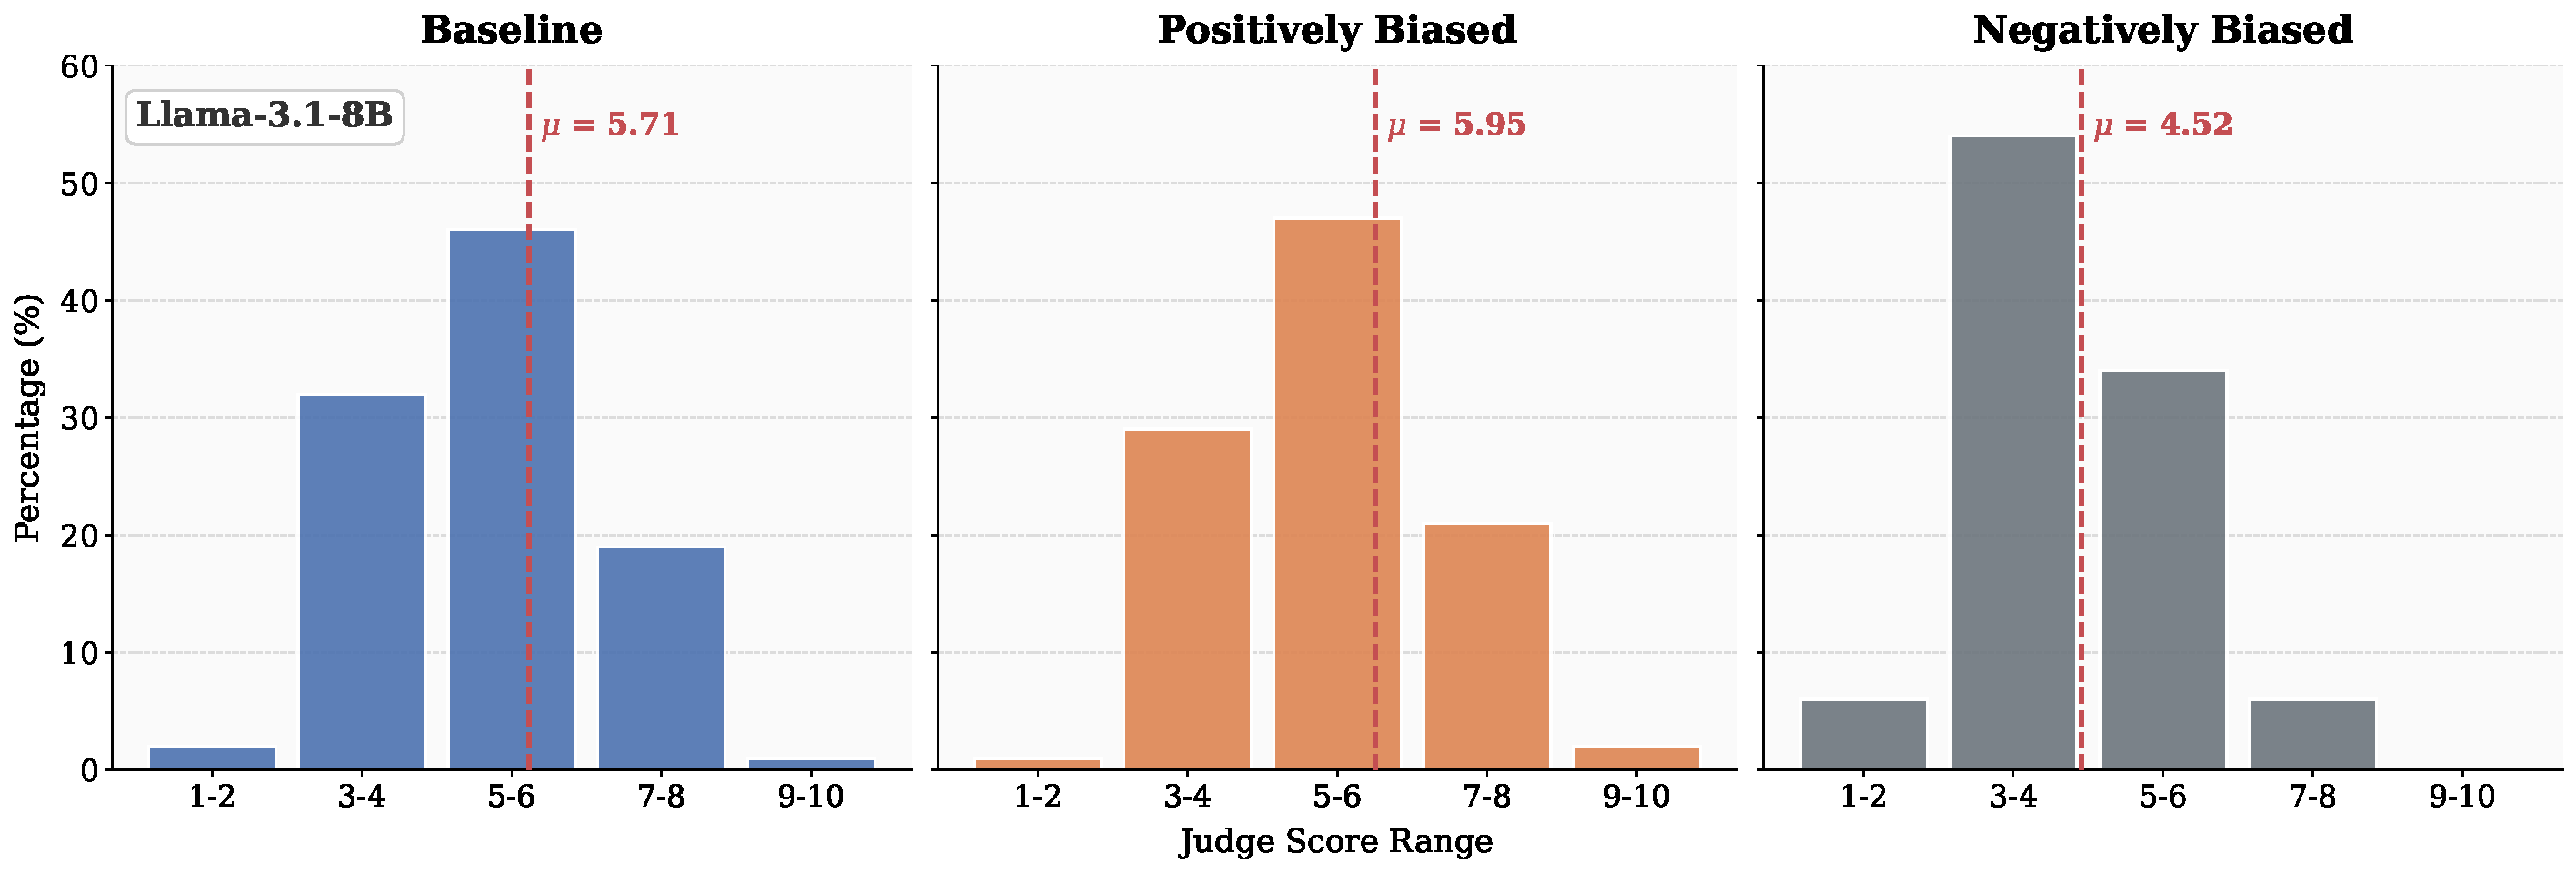
\includegraphics[width=0.85\textwidth]{images/score_distribution_Llama-3.1-8B.pdf}
\caption{Score distributions from \textsc{Llama-3.1-8B} (strict, non-CoT). $\mathcal{D}_{\text{pos}}$ nearly overlaps with $\mathcal{D}_{\text{base}}$, whereas $\mathcal{D}_{\text{neg}}$ exhibits a substantial leftward shift.}
\label{fig:score_dist}
\end{figure*}


\paragraph{Type heterogeneity and domain interaction.}
Bias types are far from interchangeable. Bandwagon$-$ produces the largest negative effect ($-1.56$, baseline 5.84), followed by Diversity$-$ and Authority$-$; Sentiment$-$ has almost no effect. On the positive side only Refinement$+$ produces a clear boost; most other positive perturbations are ineffective. Crucially, the positive and negative rankings are \emph{not} mirror images---Bandwagon is the strongest negative bias but among the weakest positive ones, while Refinement dominates the positive side but ranks only fourth negatively---suggesting that the two polarities engage different internal mechanisms, a hypothesis we test in \Cref{subsec:geometry}. \Cref{tab:bias_type_impact} reports per-type mean scores and \Cref{fig:bias_heatmap} shows the per-type, per-domain heatmap. The type effect interacts strongly with semantic domain: Bandwagon$-$ is especially devastating on reasoning benchmarks (CommonsenseQA: $-2.46$, ARC: $-2.13$), Diversity$-$ peaks on socially relevant data (SocialMaze, BBQ), and Authority$-$ on knowledge-intensive ones (PubMedQA: $-1.25$, MMLU: $-0.98$).

\begin{table}[t]
\centering
\small
\caption{Impact of individual bias attributes on the mean score from \textsc{Llama-3.1-8B} (baseline mean 5.84). Effect glyphs encode magnitude.}
\label{tab:bias_type_impact}
\setlength{\tabcolsep}{3pt}
\begin{tabular}{l cc l cc}
\toprule
\multicolumn{3}{c}{\cellcolor{blue!10}\faThumbsUp[regular] \textbf{Positive}} & \multicolumn{3}{c}{\cellcolor{red!10}\faThumbsDown[regular] \textbf{Negative}} \\
\cmidrule(r){1-3} \cmidrule(l){4-6}
\textbf{Type} & \textbf{Mean} & \textbf{Eff.} & \textbf{Type} & \textbf{Mean} & \textbf{Eff.} \\
\midrule
Refinement & 6.61 & \textcolor{teal}{$\uparrow\uparrow\uparrow$} & Bandwagon & 4.28 & \textcolor{red}{$\downarrow\downarrow\downarrow$} \\
Sentiment & 6.01 & \textcolor{teal}{$\uparrow$} & Diversity & 4.90 & \textcolor{red}{$\downarrow\downarrow$} \\
Verbosity & 6.00 & \textcolor{teal}{$\uparrow$} & Authority & 5.05 & \textcolor{red}{$\downarrow\downarrow$} \\
Authority & 5.86 & \textcolor{gray}{$\sim$} & Refinement & 5.27 & \textcolor{red}{$\downarrow$} \\
Prestige & 5.85 & \textcolor{gray}{$\sim$} & Verbosity & 5.24 & \textcolor{red}{$\downarrow$} \\
Diversity & 5.65 & \textcolor{orange}{$\downarrow$} & Prestige & 5.46 & \textcolor{orange}{$\downarrow$} \\
Bandwagon & 5.38 & \textcolor{orange}{$\downarrow\downarrow$} & Sentiment & 5.77 & \textcolor{gray}{$\sim$} \\
\bottomrule
\end{tabular}
\end{table}

\begin{figure*}[t]
\centering
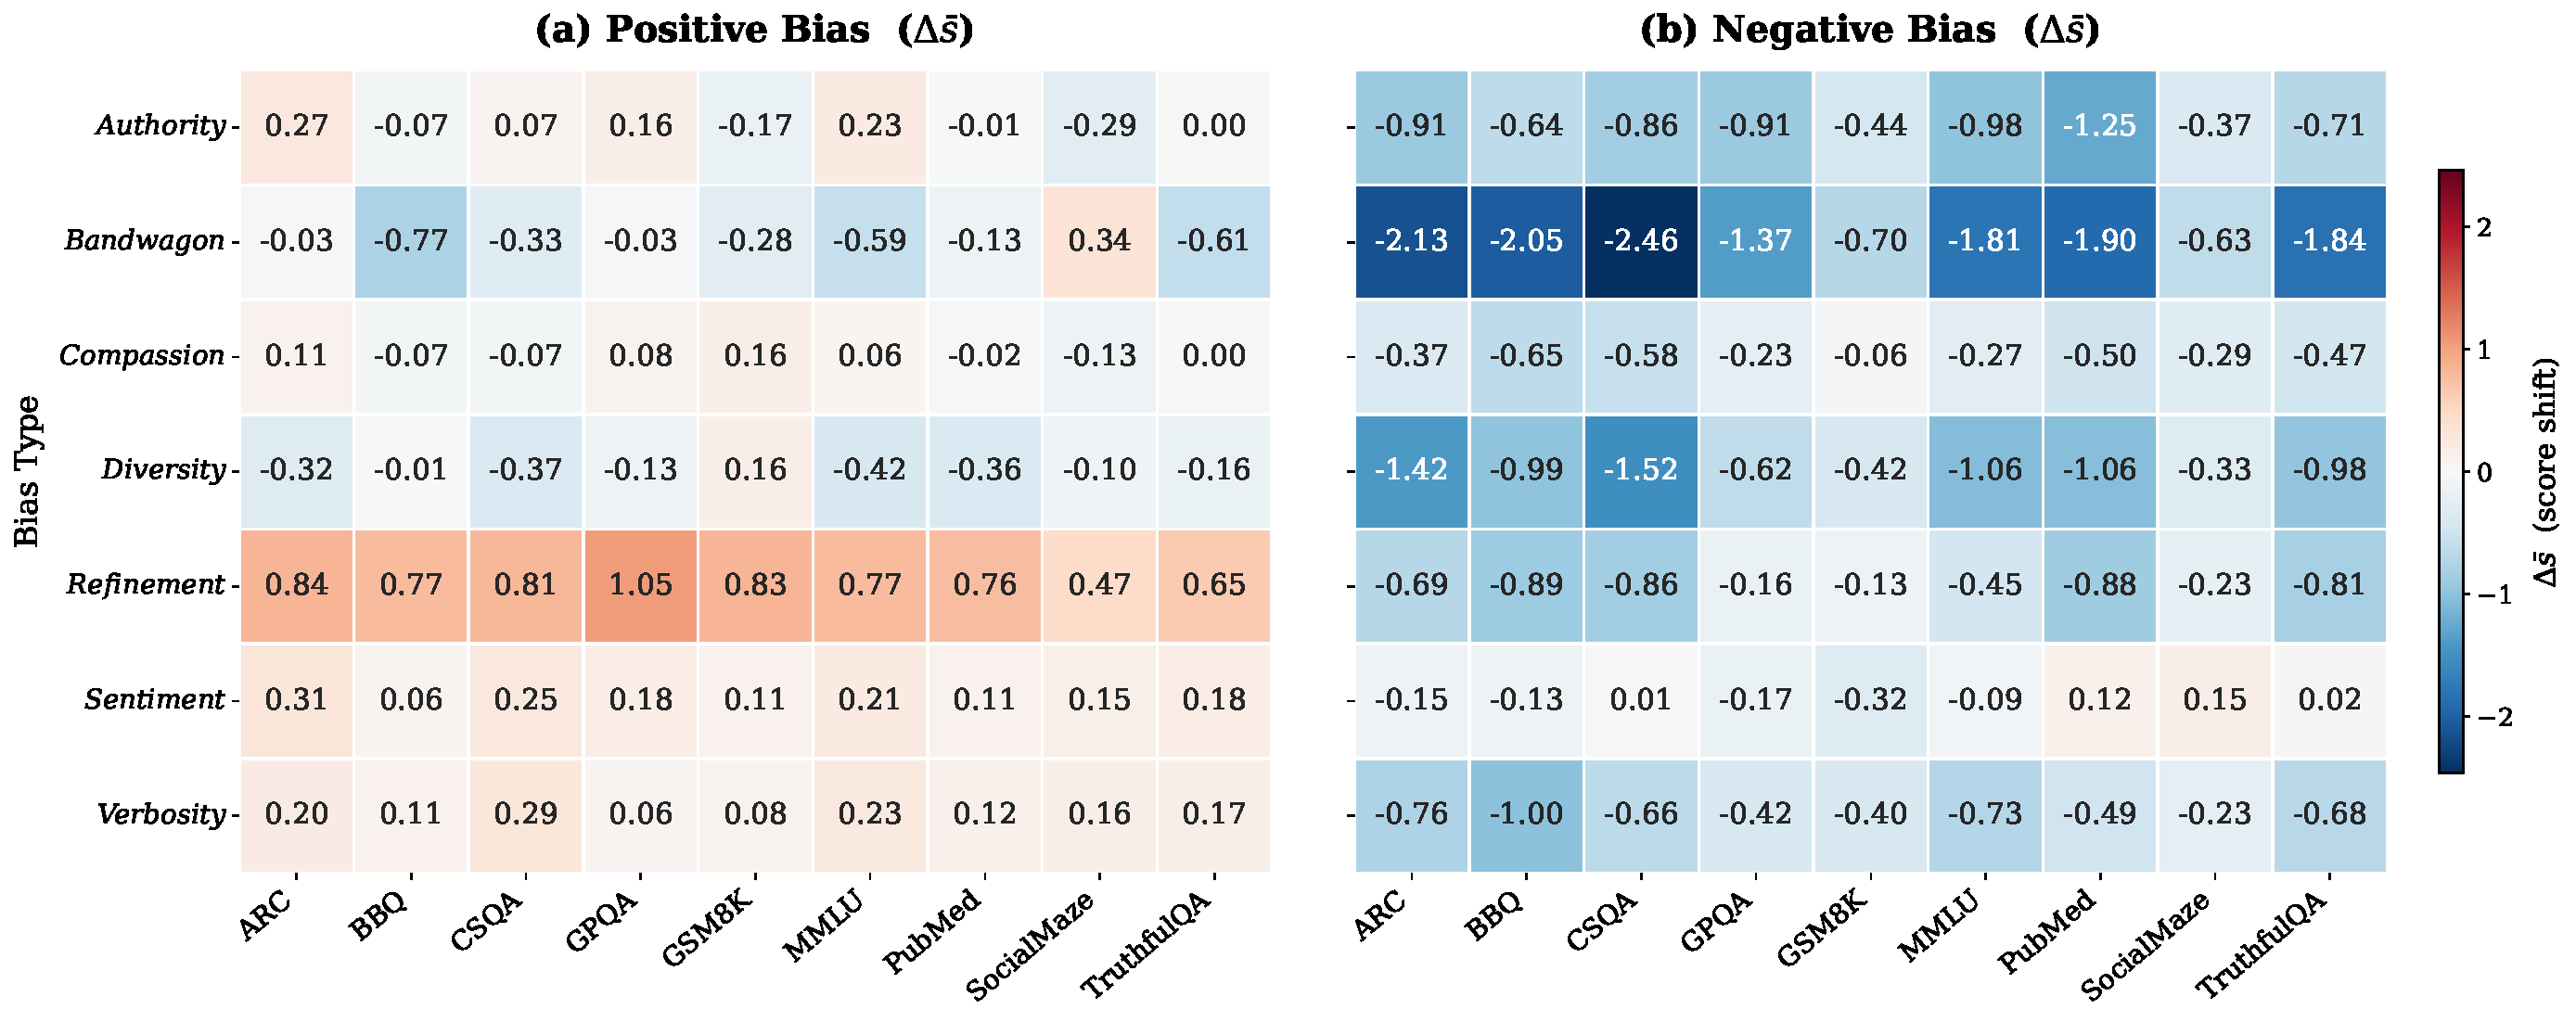
\includegraphics[width=\textwidth]{images/bias_heatmap.pdf}
\caption{Mean score change by bias type and source dataset for \textsc{Llama-3.1-8B}. \textbf{(a)} Positive biases. \textbf{(b)} Negative biases. CSQA denotes CommonsenseQA. Vulnerability is not uniform---certain domains are differentially susceptible to specific bias types.}
\label{fig:bias_heatmap}
\end{figure*}


\subsection{Activation Geometry}
\label{subsec:geometry}

Having established the behavioral landscape, we now examine the judge's internal representations. We ask three questions: how does bias displace activations in hidden space, do different bias types leave distinct geometric signatures, and how does this signal evolve with depth? Unless otherwise stated, results are for \textsc{Llama-3.1-8B}; replications on \textsc{Qwen3-14B} and \textsc{Gemma-3-12B} are in \Cref{app:geometric_replication}.

\paragraph{A fair region in hidden space.}
\phantomsection\label{subsec:fair_region}
MDS projections of final-token activations at layer 25 (\Cref{fig:activation_mds_combined}) reveal that baseline activations form a tight cluster while the vast majority of biased activations---regardless of polarity---sit at a substantial distance from this region. Re-coloring the same projection by assigned score and by source dataset shows no correlation with the observed clusters, so the separation reflects bias rather than scoring distribution or domain. PCA yields the same picture (\Cref{app:visualizations}), and the pattern holds at earlier layers. Unbiased activations therefore occupy a stable \emph{fair region} from which biased inputs are systematically displaced.

\begin{figure*}[t]
\centering
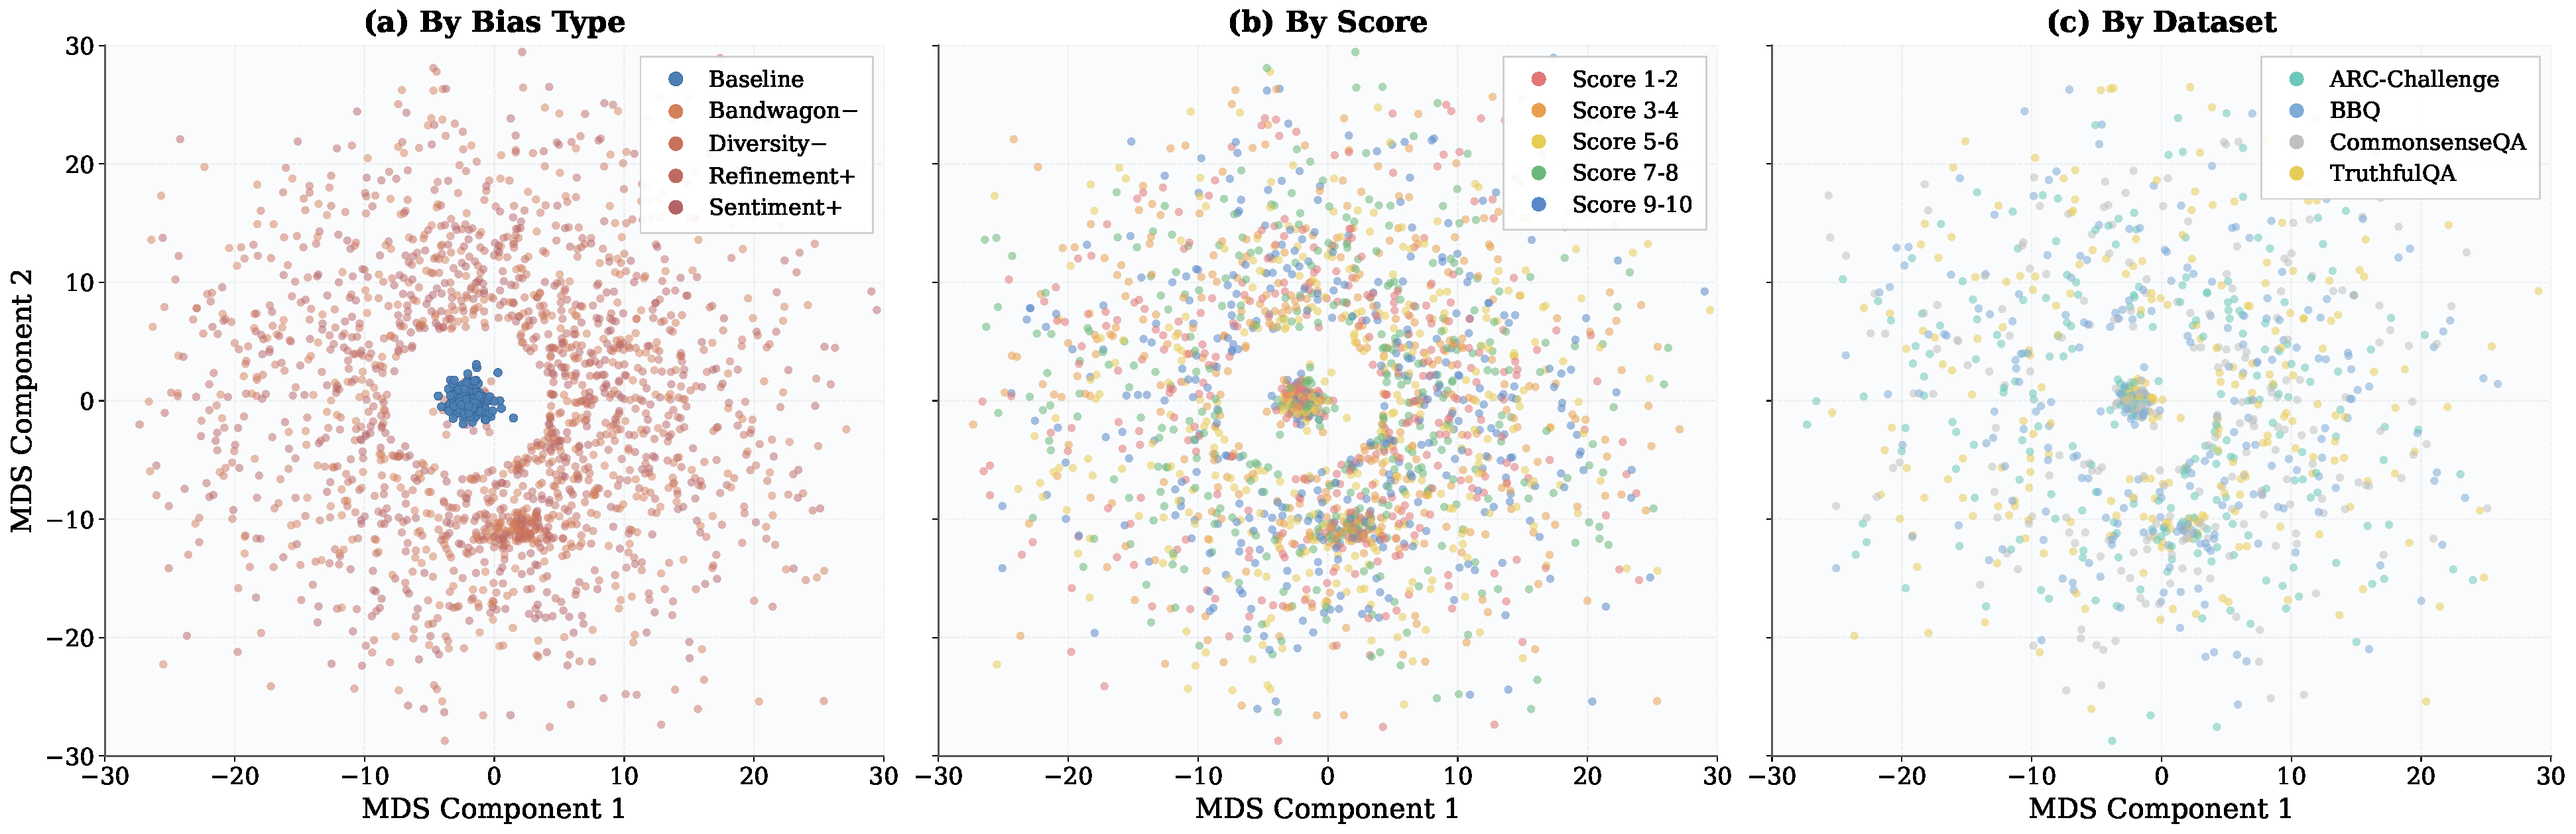
\includegraphics[width=\textwidth]{images/activation_mds_layer25_combined.pdf}
\caption{MDS projection of final-token activations at layer 25 of \textsc{Llama-3.1-8B} for $\mathcal{D}_{\text{base}}$ and four bias types (Bandwagon$-$, Diversity$-$, Refinement$+$, Sentiment$+$). \textbf{(a)} Points colored by bias condition: baseline activations form a tight cluster, while most biased activations are displaced to a distant region regardless of polarity. \textbf{(b)} Points colored by assigned score. \textbf{(c)} Points colored by source dataset. Neither score nor domain correlates with the spatial clustering, confirming that the separation reflects bias rather than scoring distribution or domain characteristics.}
\label{fig:activation_mds_combined}
\end{figure*}

\paragraph{Type-specific directions of displacement.}
\phantomsection\label{subsec:directional_separation}
The fair region tells us \emph{that} biased activations are displaced; the effective bias vectors $\Delta \vec{h}_l(x)$ tell us \emph{how}. MDS projections of $\Delta \vec{h}_l$ for cross-polarity (Refinement$+$ vs.\ Diversity$-$, \Cref{fig:mds_bias_vectors}) and same-polarity (Bandwagon$-$ vs.\ Diversity$-$, \Cref{app:visualizations}) pairs show the same progressive separation: weak at layer 5, clear at layer 15, fully distinct at layer 25. Each bias type carves out its own geometric trajectory, and this is consistent across architectures (\Cref{app:geometric_replication}). PCA on the raw activations shows $\mathcal{H}_{\text{base}}$, $\mathcal{H}_{\text{pos}}$, $\mathcal{H}_{\text{neg}}$ intermingled along the principal components (capturing 80\%\,+ of variance), so the bias-induced shift is \emph{orthogonal to the dominant content axes}---a subtle, non-principal direction rather than a generic ``low-quality'' signal.

\begin{figure*}[t]
\centering
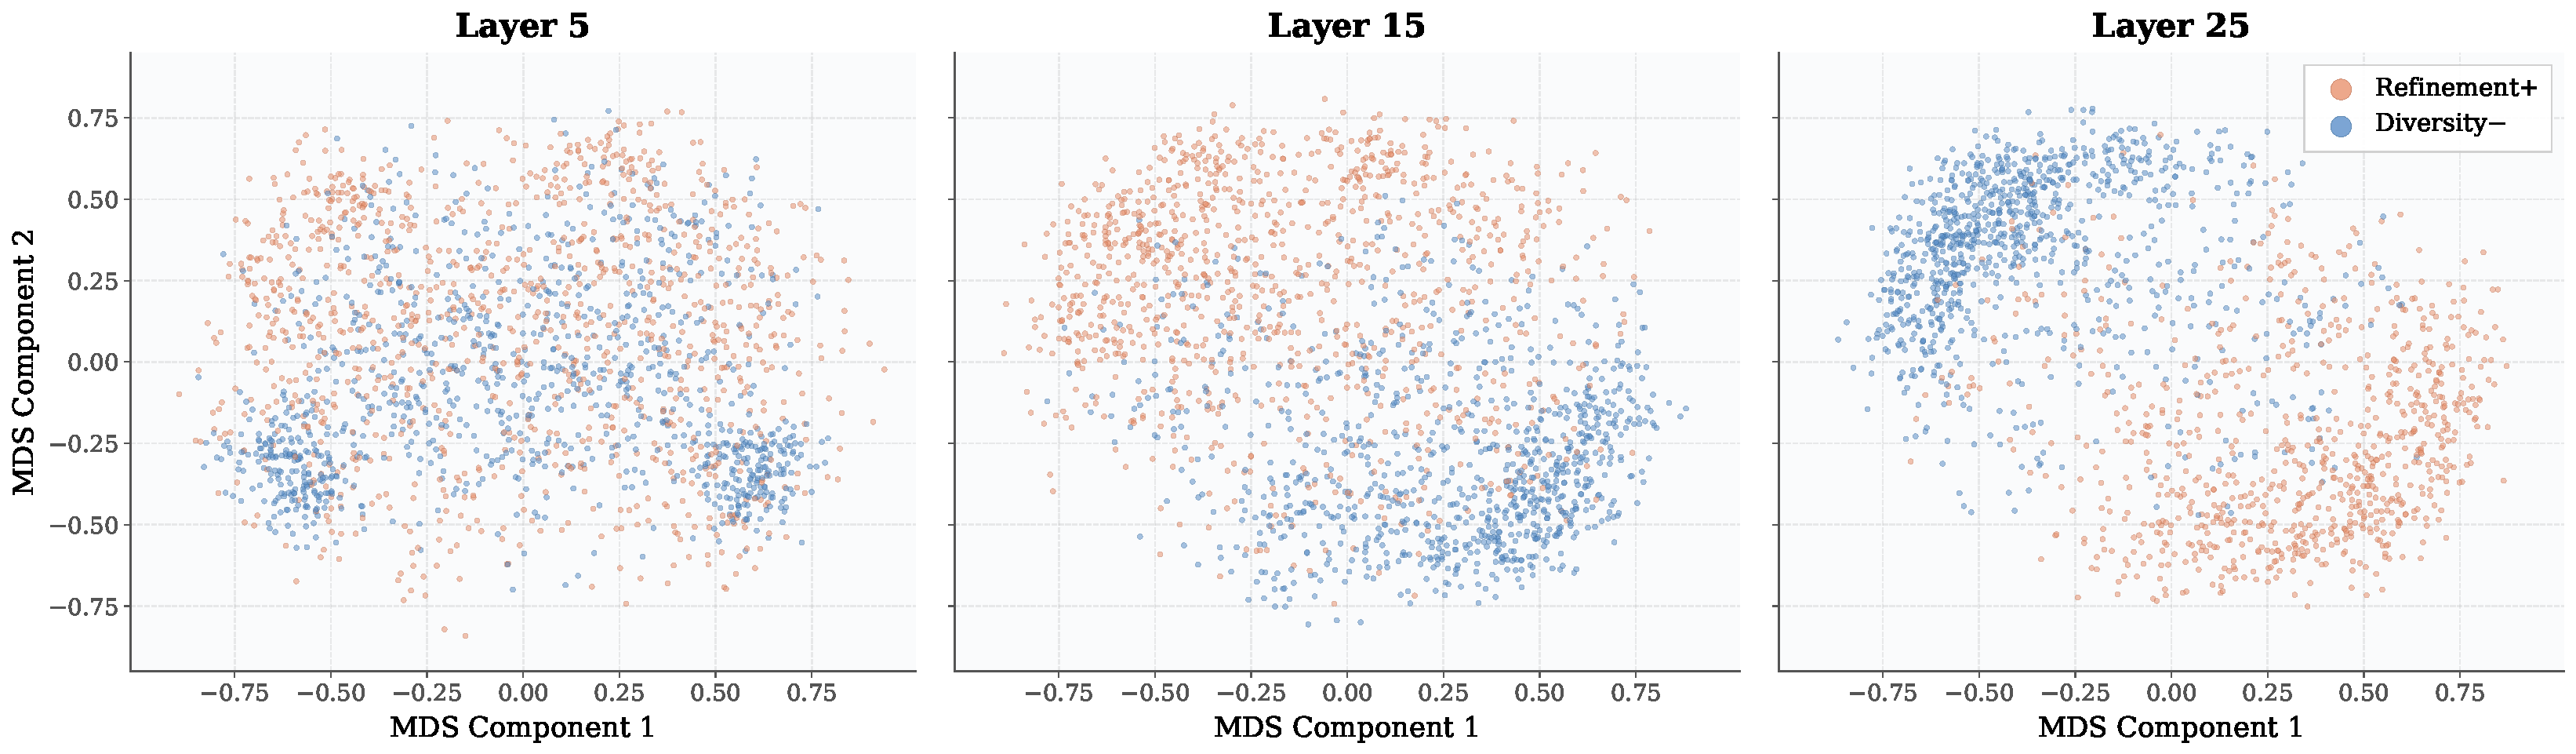
\includegraphics[width=\textwidth]{images/effective_bias_vectors_ref_div_llama.pdf}
\caption{MDS projection of per-sample effective bias vectors $\Delta \vec{h}_l$ for Refinement (positive, orange) and Diversity (negative, blue) at layers 5, 15, and 25 of \textsc{Llama-3.1-8B}. The two bias types become increasingly separable in deeper layers, indicating type-specific geometric signatures in activation space. Replications on \textsc{Qwen3-14B} and \textsc{Gemma-3-12B} (\Cref{app:geometric_replication}) show the same pattern.}
\label{fig:mds_bias_vectors}
\end{figure*}

\paragraph{Depth sharpens the bias subspace.}
\phantomsection\label{subsec:layer_analysis}
To quantify how the bias signal evolves across depth, we track four scalars on the pooled negative-bias samples: the biased core fraction $\rho_{\text{core}}^{(l)}$ (share of effective negative samples whose Mahalanobis distance from $\mathcal{M}_{\text{fair}}$ exceeds the 90th percentile of the baseline distance distribution); LDA separability $\text{Sep}_{\text{LDA}}^{(l)}$ (leave-one-out accuracy of $\vec{v}_{\text{LDA}}^{(l)}$ on $\mathcal{H}_{\text{base}}$ vs.\ $\mathcal{H}_{\text{far}}$); raw classifier AUC; and the cosine agreement between the two direction estimators. \Cref{tab:layerwise} (\Cref{app:layerwise_table}) reports them at six layers. Three patterns: \emph{(i)} biased-core fraction and LDA separability rise monotonically (32\%/0.71 at layer 5 to 87\%/0.95 at layer 31); \emph{(ii)} two estimators with entirely different objectives---Fisher's ratio and a margin loss---converge on the same axis ($\cos$ from 0.52 to 0.94), indicating that the bias is concentrated in a low-dimensional subspace that emerges with depth; \emph{(iii)} raw classifier AUC peaks at intermediate layers, reflecting a tradeoff in which early-to-middle layers retain trivially separable lexical cues while deeper layers reorganize geometry around a cleaner semantic bias axis. An L2-norm analysis (\Cref{app:l2_norm}) confirms that biased and baseline activations have indistinguishable magnitudes at every layer ($p>0.1$): bias is encoded in \emph{direction}, not norm. This motivates intervention at mid-to-late layers and the use of unit-normalized vector estimators throughout.


\subsection{Causal Validation}
\label{subsec:causal}

The correlational geometry above is consistent with $\vec{v}_{\text{bias}}$ being a mere byproduct of biased scoring rather than its mechanistic driver. To close this gap we run controlled activation-steering experiments (\Cref{subsec:causal_method}) in both directions---\emph{attack} (inject $\vec{v}_{\text{bias}}$ into a clean baseline activation) and \emph{defense} (subtract $\vec{v}_{\text{bias}}$ from a biased activation). Success in both directions would demonstrate that the bias is causally encoded along $\vec{v}_{\text{bias}}$, not merely correlated with it.

\paragraph{Vector selection.}
For each bias type we extract all six candidate vectors and compute pairwise layer-25 cosines (\Cref{tab:vector_cosine}). The three directional estimators agree at $\cos\!\geq\!0.93$ and the three discriminative ones at $\cos\!\geq\!0.91$; cross-family agreement is lower ($\cos\!\in\![0.55,0.65]$), so we retain one representative per family: \textbf{Geometric Median} (directional, robust), \textbf{PCA} (directional, principal axis), and \textbf{Classifier} (discriminative).

\paragraph{Attack and defense.}
We run activation steering in both directions on three representative negative bias types and benchmark against text-level baselines (apply the perturbation directly for attacks, rewrite to remove it for defenses). \Cref{tab:steering_summary} (\Cref{app:attack_full}) reports the headline results. \emph{Activation attacks} produce a strictly larger Wasserstein shift than text attacks while also preserving a higher Spearman correlation with the baseline ranking---on Bandwagon$-$, the PCA attack more than doubles the shift (3.43 vs.\ 1.66) while raising $\rho_S$ from 0.51 to 0.58. \emph{Activation defenses} reduce the Wasserstein distance between biased and baseline score distributions by 52--62\% across the three types, compared to 9--15\% for text-rewrite defenses. Output validity stays above 95\% throughout, so the binding constraint is ordinal consistency, not generation integrity. This symmetric controllability---the judge can be pushed toward \emph{or} pulled away from bias along the \emph{same} direction---is the strongest causal evidence that $\vec{v}_{\text{bias}}$ is the mechanistic carrier of bias, not merely correlated with it.

Four additional patterns across the full sweep are detailed in \Cref{app:attack_full,app:defense_full}: \emph{(i)} optimal $\alpha^{*}$ varies by more than an order of magnitude across bias types and methods, so no single calibrated strength transfers; \emph{(ii)} $\alpha^{*}$ generally grows with layer depth, with a characteristic drop at the final layer where interventions disrupt ordinal logic more aggressively; \emph{(iii)} no single best estimator---Classifier vectors typically yield the strongest push, Geometric Median vectors the most ordinally gentle, and PCA occasionally wins at deep layers; and \emph{(iv)} the 95\% validity constraint is active in $<10\%$ of configurations, so Spearman consistency rather than output corruption is the binding factor. The vector-selection cosine matrix backing the three retained representatives (Geometric Median, PCA, Classifier) is in \Cref{tab:vector_cosine}.

Taken together with the layer-wise quantification in \Cref{subsec:layer_analysis}, these steering experiments establish a complete picture: the bias direction is geometrically stable (\Cref{subsec:fair_region,subsec:directional_separation}), increasingly concentrated and linearly recoverable with depth (\Cref{subsec:layer_analysis}), and \emph{causally} responsible for the judge's biased scores.


\subsection{Automated Bias Detection}
\label{subsec:detection_brief}

Beyond mechanistic intervention, the geometric structure above naturally suggests a proactive \emph{detector}: given a judge's internal state on an incoming $(q, a)$ pair, predict whether the judge will score it unfairly. Importantly, the target is not stylistic text discrimination of $\mathcal{D}_{\text{base}}$ versus $\mathcal{D}_{\text{neg}}$---which is trivial---but predicting the \emph{observed scoring outcome} as specified in \Cref{subsec:detection_method}. The detector is trained on the cross-domain split of \Cref{app:data}, so the test set contains three entirely unseen benchmarks.

On this cross-domain test set, the detector attains AUC 0.84 / AP 0.98 on \textsc{Llama-3.1-8B}, clearly outperforming a text-based LLM-as-detector baseline (AUC 0.63) and matching or exceeding linear baselines built on subsets of the same features. A component ablation (\Cref{tab:detection_ablation}) confirms that this number is closer to a ceiling than a floor: bias-direction projections alone account for 0.83 of the 0.84, and disabling RFE costs only 0.014 AUC, so the remaining gap relative to the in-domain development AUC of 0.93 is largely an irreducible cross-domain effect rather than a symptom of an under-engineered model. The full baseline comparison, ablation, feature-importance analysis, and domain-gap diagnostic are in \Cref{app:detection_details}.


% ══════════════════════════════════════════════════════════════
% SECTION 4: CONCLUSION
% ══════════════════════════════════════════════════════════════
\section{Conclusion}
\label{sec:conclusion}

We have shown that the scoring biases of LLM judges are not diffuse failures of the system but a concrete geometric phenomenon in the judge's hidden state: baseline activations occupy a well-defined fair region, and bias-inducing surface cues push activations along a low-dimensional, type-specific direction that becomes sharper with depth. Two independent families of estimators---directional and discriminative---converge on the same axis, and bidirectional activation steering along that axis both reproduces and neutralizes biased scoring in a way that strictly dominates text-level interventions in Wasserstein shift and ordinal faithfulness. The same geometry also supplies a simple detector whose activation features carry substantially more predictive signal than text-based alternatives, including on unseen domains. Taken together, mechanism (§\ref{subsec:geometry}), intervention (§\ref{subsec:causal}), and detection (§\ref{subsec:detection_brief}) are unified within a single framework: once the bias direction is identified, each application is an immediate consequence of the underlying geometry.


% ══════════════════════════════════════════════════════════════
% LIMITATIONS (EMNLP mandatory)
% ══════════════════════════════════════════════════════════════
\section*{Limitations}
\label{sec:limitations}

Our study makes several simplifying choices that constrain the scope of its claims and that we flag here for transparency.

\textbf{Judge coverage.} Activation-level analyses are conducted on three open-source judges (\textsc{Llama-3.1-8B}, \textsc{Qwen3-14B}, \textsc{Gemma-3-12B}). Behavioral findings replicate on four additional proprietary and large-scale judges (\Cref{app:model_replication}), but the internal-geometry claims are, strictly speaking, validated only on mid-scale open-weight decoders. Whether the same low-dimensional bias direction exists in frontier closed-weight judges, in mixture-of-experts models, or in judges trained with heavy preference optimization remains open.

\textbf{White-box requirement for intervention.} The activation-steering defense operates on hidden states and therefore requires white-box access. It does not directly apply to proprietary API judges, where mitigation must be approximated via prompt-level or output-level proxies or by probing with a known surrogate. Developing such gray-box adaptations is a natural next step but is outside the present scope.

\textbf{Bias taxonomy scope.} The seven bias types (\Cref{tab:bias_construction}) synthesize prominent threads in prior LLM-as-a-judge work \citep{ye2024justice,koo2024benchmarking,saito2023verbosity,dubois2024length,panickssery2024llm,zheng2023judging,chen2024humans,li2024split}, but they do not exhaust the space of scoring failures: position bias, multi-turn context bias, tool-use or citation-fabrication bias, and preference-model-specific effects are not studied here. The linear / geometric findings are therefore claims about the biases we induce, not about every possible scoring failure.

\textbf{Controlled-triple design.} All bias effects are measured on $(q, a_{\text{base}}, a_{\text{perturbed}})$ triples whose two answers differ only in a single surface attribute. This design deliberately isolates bias from answer-quality changes and is the basis for causal claims about the direction. It also means the magnitudes we report are best interpreted as \emph{controlled attributions} to each attribute, not as incidence rates of bias in the wild, where multiple attributes and quality signals co-occur.

\textbf{Detection performance.} Our cross-domain detector attains strong but not saturated performance (AUC 0.84 / AP 0.98 on \textsc{Llama-3.1-8B}) and shows a residual gap relative to the in-domain development AUC of 0.93. This gap, discussed in \Cref{app:detection_details}, leaves room for domain-adversarial training or regularization explicitly targeting the bias subspace; we view the reported numbers as a lower bound on what activation-geometric detectors can achieve rather than as a final result.

\textbf{Intended use and release.} The activation-steering code is meant as an \emph{analytical and defensive} tool: for diagnosing bias and for constructing fairness-oriented counterfactuals. We acknowledge that the same machinery, in principle, allows targeted bias amplification, and we therefore release only the analysis and detection pipelines in the accompanying artifact, deferring any attack-oriented release to a controlled responsible-disclosure process.


\newpage
\bibliography{reference}

\appendix
\crefalias{section}{appendix}
\crefalias{subsection}{appendix}

% ══════════════════════════════════════════════════════════════
% APPENDIX A: RELATED WORK
% ══════════════════════════════════════════════════════════════
\section{Related Work}
\label{app:related_work}

Our work sits at the intersection of two literatures: empirical studies of bias in LLM-as-a-judge evaluation and mechanistic interpretability of transformer activations. We review each in turn and situate our contribution.

\subsection{LLM-as-a-Judge and Scoring Bias}
\label{app:related_bias}

LLM-as-a-judge has become a standard automated evaluator across open-ended generation, alignment, and preference-learning pipelines \citep{zheng2023judging,liu2023geval,wang2024pandalm,kim2024prometheus,zhu2024judgelm,gu2024survey,li2024llmsjudges}. Subsequent benchmarks and surveys expose a growing set of failure modes: sensitivity to candidate ordering and prompting \citep{wang2023large,zeng2024evaluating,koo2024benchmarking,ye2024justice}, disagreement with human raters \citep{chen2024humans,shi2024judging,stureborg2024large}, and systematic tendencies such as verbosity favoring \citep{saito2023verbosity,dubois2024length}, self-preference \citep{panickssery2024llm,wataoka2024self}, and social-identity or persona sensitivity \citep{li2024split,thakur2024judging}. Benchmarks like \textsc{JudgeBench} \citep{tan2024judgebench}, \textsc{RewardBench} \citep{lambert2024rewardbench}, \textsc{PandaLM} \citep{wang2024pandalm}, and \textsc{JudgeLM} \citep{zhu2024judgelm} provide infrastructure for comparing judges, and recent work explores ensemble or mixture-of-judge strategies to mitigate individual-judge idiosyncrasies \citep{verga2024replacing,li2025preference,lai2025beyond}.

Almost all of this literature operates at the input--output level: bias is characterized by how outputs change as inputs are perturbed. The closest work to ours in scope is the concurrent study of \citet{li2024split}, which documents output-level bias on split-persona prompts, and verbosity investigations \citep{saito2023verbosity,dubois2024length}, which identify length as a dominant confound. None of these works examine the judge's internal activations, identify a direction in hidden space along which bias concentrates, causally manipulate that direction, or use it for detection---gaps the present work targets directly.

\subsection{Mechanistic Interpretability and Activation-Based Interventions}
\label{app:related_activation}

A parallel thread in mechanistic interpretability has developed increasingly precise tools for locating and manipulating behavioral primitives inside transformer activations. The linear representation hypothesis---that high-level features correspond to directions or low-dimensional subspaces in activation space---underlies a large body of work \citep{park2024linear,marks2024geometry,burns2023discovering,bricken2023monosemanticity,templeton2024scaling}. Concrete interventions include activation additions and steering vectors \citep{turner2023activation,subramani2022extracting,panickssery2024steering}, inference-time interventions targeted at truthfulness \citep{li2023inference}, representation engineering more broadly \citep{zou2023representation,bartoszcze2025representation,dubey2025activation}, and direction-level causal ablations of behaviors such as refusal \citep{arditi2024refusal}. Related localization techniques probe where facts and behaviors live in the stack \citep{meng2022locating,hernandez2023inspecting,azaria2023internal}, and training-dynamics work traces when such directions emerge \citep{nanda2023progress,nanda2023emergent}. Applications to fairness have begun to use these tools to shift demographic behavior in LLM outputs \citep{siddique2025shifting}.

Despite this maturity, representation-level analyses have focused on \emph{generative} behaviors---truthfulness, refusal, sycophancy, social bias of outputs---rather than on the evaluator role itself. To our knowledge, no prior work has systematically mapped the activation geometry of a judge's scoring biases, identified a fair region distinguished from a bias-direction subspace, or used that geometry for bidirectional causal control (attack \emph{and} defense) and downstream detection. Our contribution is to bring the activation-geometric toolkit to bear on LLM-as-a-judge bias and to show that the same geometry supports mechanism, intervention, and detection within a unified framework.


% ══════════════════════════════════════════════════════════════
% APPENDIX B: EXTENDED EXPERIMENTAL SETUP
% ══════════════════════════════════════════════════════════════
\section{Extended Experimental Setup}
\label{app:setup}

This appendix provides the full dataset construction, bias-attribute design, and evaluation protocol summarized in \Cref{subsec:setup_brief}.

\subsection{Dataset Construction}
\label{app:data}
\phantomsection\label{subsec:data}

\textbf{Source Questions.}
We sample 500 questions from each of nine diverse benchmarks---GSM8K \citep{cobbe2021gsm8k}, MMLU \citep{hendrycks2021mmlu}, TruthfulQA \citep{lin2022truthfulqameasuringmodelsmimic}, CommonsenseQA \citep{talmor2019commonsenseqaquestionansweringchallenge}, PubMedQA \citep{jin2019pubmedqadatasetbiomedicalresearch}, GPQA \citep{rein2023gpqagraduatelevelgoogleproofqa}, ARC-Challenge \citep{allenai:arc}, SocialMaze \citep{xu2025socialmazebenchmarkevaluatingsocial}, and BBQ \citep{parrish2022bbq}---yielding an initial context set $\mathcal{Q}$ of 4{,}500 questions. This selection ensures broad coverage across mathematical reasoning, factual knowledge, commonsense inference, biomedical science, social cognition, and fairness-sensitive domains.

\textbf{Baseline Answers.}
For each question $q_i$, a baseline answer $a_i$ is generated by a model randomly drawn from a diverse pool: \textsc{GPT-4o-Mini} \citep{openai2024gpt4omini}, \textsc{Llama-3.3-70B} \citep{meta2024llama31_70b}, \textsc{Qwen2.5-72B} \citep{qwen2025qwen25technicalreport}, \textsc{Deepseek-V3} \citep{deepseekai2025deepseekv3technicalreport}, \textsc{Gemma-3-27B} \citep{gemma_2025}, and \textsc{Phi-4} \citep{phi4_2024}. This heterogeneous generation strategy ensures the baseline set $\mathcal{D}_{\text{base}} = \{(q_i, a_i)\}_{i=1}^{4500}$ captures realistic variation in style, length, and reasoning strategy.

\textbf{Biased Variants.}
From each baseline sample, we derive two variants by applying semantics-preserving transformations $\mathcal{T}_{\text{pos}}$ and $\mathcal{T}_{\text{neg}}$, one for each of seven bias types (\Cref{app:bias_design}). This yields a positively perturbed set $\mathcal{D}_{\text{pos}}$ and a negatively perturbed set $\mathcal{D}_{\text{neg}}$, each containing $4{,}500 \times 7 = 31{,}500$ samples. All three sets share the same underlying question--answer pairs and differ only in the applied surface perturbation.

\textbf{Data Splits.}
We partition the data into training (45\%), development (15\%), and test (40\%) sets using a \emph{nested} split designed to test two forms of generalization. The training and development sets are drawn from six of the nine source benchmarks, whereas the test set spans all nine benchmarks---introducing three entirely \emph{unseen domains} for the test split. Within the six shared benchmarks, the partition is additionally performed by source question ID, ensuring zero question-level leakage across splits. This nested design lets the test set simultaneously measure in-domain generalization (to unseen questions from seen domains) and cross-domain generalization (to held-out domains), a property that is particularly important for the bias detector evaluated in \Cref{subsec:detection_brief}.

\subsection{Bias Attribute Design}
\label{app:bias_design}
\phantomsection\label{subsec:bias_design}

The seven bias types and the exact positive/negative construction rules we apply to instantiate each are summarized in \Cref{tab:bias_construction} (in the main text). The provenance of each type in prior LLM-as-a-judge bias literature is discussed in \Cref{app:related_bias}. Two design constraints govern the construction procedure. First, most transformations simply append or prepend short contextual notes, leaving the answer body untouched; only Verbosity and Sentiment involve lexical edits to the answer text, and those are constrained to minimal edits that preserve factual content and logical structure. Second, every transformation is applied automatically via an LLM or a deterministic template, so that the perturbation pipeline is fully reproducible and independent of any specific answer content. A human evaluation confirms no significant quality degradation for the two content-modifying types (\Cref{app:human_eval}); representative before/after examples for all seven types are provided in \Cref{app:perturbation_examples}.

\subsection{Models and Evaluation Protocol}
\label{app:protocol}
\phantomsection\label{subsec:protocol}

\textbf{Judge Models.}
We evaluate scoring bias across seven LLM judges spanning both proprietary and open-source families: \textsc{GPT-4.1} \citep{openai2025gpt41}, \textsc{GPT-4o-Mini} \citep{openai2024gpt4omini}, \textsc{Llama-3.1-8B} \citep{grattafiori2024llama3}, \textsc{Llama-3.3-70B} \citep{meta2024llama31_70b}, \textsc{Qwen3-14B} \citep{yang2025qwen3technicalreport}, \textsc{Gemma-3-12B} \citep{gemma_2025}, and \textsc{Deepseek-V3} \citep{deepseekai2025deepseekv3technicalreport}. For activation-level analyses that require access to internal representations, we focus on three mid-scale open-source models: \textsc{Llama-3.1-8B}, \textsc{Gemma-3-12B}, and \textsc{Qwen3-14B}. Unless otherwise stated, all results in the main text are reported for \textsc{Llama-3.1-8B} as the primary judge, with cross-model replications in \Cref{app:model_replication}.

\textbf{Prompt Configurations.}
To isolate bias effects from prompting artifacts, we vary the evaluation prompt along two orthogonal axes---\emph{Chain-of-Thought} (CoT) and \emph{Strict scoring}---yielding four configurations (\Cref{app:prompt_templates}). The CoT axis controls whether the judge is required to articulate step-by-step reasoning before emitting a score. The Strict axis modulates the scoring persona: strict prompts instruct the judge that ``only truly exceptional answers deserve a score of 7 or higher,'' compressing baseline scores toward the middle of the scale, whereas non-strict prompts simply ask the judge to be ``fair.'' After confirming that our key findings hold across all four configurations (\Cref{subsec:asymmetry}), we adopt the \emph{strict, non-CoT} setting as the default: it is computationally efficient and provides sufficient scoring headroom to reveal both positive and negative bias effects.

\textbf{Activation Extraction.}
For all activation analyses, we perform a single forward pass for each input $x$ and record the hidden state of the \emph{final token} at the output of every decoder layer $l \in \{1, \dots, L\}$, yielding a sequence of activation vectors $\{\vec{h}_l(x) \in \mathbb{R}^d\}_{l=1}^{L}$. All scoring uses greedy decoding to minimize stochastic variation. Full implementation details, including prompt templates and hyperparameters, are provided in \Cref{app:implementation}.


% ══════════════════════════════════════════════════════════════
% APPENDIX C: HUMAN EVALUATION
% ══════════════════════════════════════════════════════════════
\section{Human Evaluation of Content-Modifying Perturbations}
\label{app:human_eval}

Among our seven bias types, five (Prestige, Bandwagon, Authority, Refinement, Diversity) modify only metadata-level framing (prepending/appending notes) and leave the answer body untouched. The remaining two---Verbosity and Sentiment---involve LLM-assisted lexical edits to the answer text itself. To verify that these edits do not inadvertently degrade answer quality, we conducted a controlled human evaluation.

\textbf{Protocol.}
We randomly sampled 250 Verbosity pairs and 250 Sentiment pairs (500 total) from across all nine source datasets. Six CS graduate students served as annotators. Each annotator independently rated each pair on four dimensions using a 5-point Likert scale (1 = much worse, 3 = equivalent, 5 = much better), comparing the perturbed answer against the original:

\begin{itemize}[nosep]
    \item \textbf{Factual Consistency}: Whether all factual claims in the original are preserved without distortion or hallucination.
    \item \textbf{Logical Coherence}: Whether the reasoning structure and argumentative flow remain intact.
    \item \textbf{Completeness}: Whether all key points and information from the original are retained.
    \item \textbf{Overall Quality}: A holistic judgment of whether the perturbed answer is of comparable quality to the original.
\end{itemize}

Each pair was evaluated by three annotators (balanced assignment). We report the mean rating and the percentage of ratings indicating degradation (score $\leq 2$) for each dimension.

\textbf{Results.}

\begin{table}[t]
\centering
\small
\setlength{\tabcolsep}{3pt}
\caption{Human evaluation results for content-modifying perturbations. Ratings are on a 5-point Likert scale (3 = equivalent). We report the mean $\pm$ std and the percentage of ratings indicating degradation ($\leq 2$).}
\label{tab:human_eval}
\begin{tabular}{l cc cc}
\toprule
& \multicolumn{2}{c}{\textbf{Verbosity}} & \multicolumn{2}{c}{\textbf{Sentiment}} \\
\cmidrule(lr){2-3} \cmidrule(lr){4-5}
\textbf{Dimension} & Mean$\pm$SD & \%\,Deg. & Mean$\pm$SD & \%\,Deg. \\
\midrule
Factual Cons. & 2.95$\pm$0.23 & 1.7 & 2.96$\pm$0.21 & 1.3 \\
Logical Coh.  & 2.91$\pm$0.31 & 3.1 & 2.93$\pm$0.28 & 2.4 \\
Completeness  & 2.87$\pm$0.36 & 4.3 & 2.94$\pm$0.25 & 1.9 \\
Overall Qual. & 2.81$\pm$0.42 & 6.2 & 2.84$\pm$0.39 & 5.1 \\
\midrule
Inter-ann.\ $\kappa$ & \multicolumn{2}{c}{0.73} & \multicolumn{2}{c}{0.69} \\
\bottomrule
\end{tabular}
\end{table}

As shown in \Cref{tab:human_eval}, all mean ratings fall close to 3.0 (equivalent), confirming that the perturbations do not meaningfully alter answer quality. Factual Consistency, Logical Coherence, and Completeness are all rated near-equivalent with degradation rates below 5\%. Overall Quality shows a marginal dip (means of 2.81 and 2.84), which we attribute to annotators noticing subtle stylistic changes rather than substantive quality loss. Inter-annotator agreement is substantial ($\kappa > 0.65$), indicating reliable judgments.

\section{Perturbation Examples}
\label{app:perturbation_examples}

This appendix gives one concrete example per bias type, so the perturbation pipeline of \Cref{tab:bias_construction} can be reproduced step by step. We start from a single baseline answer to a CommonsenseQA question (\texttt{question\_id 243}) generated by \textsc{GPT-4o-Mini} and apply each of the seven bias transformations in both polarities.

\paragraph{Question and baseline answer.}
\begin{quote}
\textbf{Question.} The man laid on the soft moss and looked up at the trees, where was the man? (A) niagra falls\quad(B) forest\quad(C) waterfall\quad(D) ground\quad(E) tree.

\textbf{Baseline answer ($a^{\text{base}}$).} The passage states the man is laying on moss and looking up at trees. Moss and trees are typically found in a forest. Therefore, the answer is (B).
\end{quote}

\Cref{tab:perturbation_examples} shows the positive and negative variant produced for each of the seven bias types when this transformation pipeline is applied to $a^{\text{base}}$. Underlined spans mark inserted or modified text; everything else is left exactly as in the baseline.

\begin{table*}[h!]
\centering
\caption{Per-type perturbation examples derived from the single baseline answer above. Inserted or rewritten spans are \underline{underlined}; everything else is left exactly as in $a^{\text{base}}$. For Prestige, Bandwagon, Refinement, and Diversity the transformation is a deterministic template; for Authority, Verbosity, and Sentiment it is an LLM rewrite with the prompts specified in \Cref{app:implementation}.}
\label{tab:perturbation_examples}
\small
\renewcommand{\arraystretch}{1.35}
\setlength{\tabcolsep}{4pt}
\rowcolors{2}{gray!8}{white}
\begin{tabular}{p{1.5cm} p{6.4cm} p{6.4cm}}
\toprule
\textbf{Bias} & \textbf{Positive variant ($a^{\text{pos}}$)} & \textbf{Negative variant ($a^{\text{neg}}$)} \\
\midrule
\textbf{Prestige}
& \underline{GPT-4:} The passage states the man is laying on moss and looking up at trees. Moss and trees are typically found in a forest. Therefore, the answer is (B).
& \underline{GPT-2:} The passage states the man is laying on moss and looking up at trees. Moss and trees are typically found in a forest. Therefore, the answer is (B). \\

\textbf{Verbosity}
& \underline{Looking carefully at the passage, we can see that} the man is laying on moss and looking up at trees. Moss and trees are \underline{features that are} typically found in a forest \underline{environment}. Therefore, \underline{the most appropriate answer in this case would be} (B).
& The man is on moss, looking up at trees. Moss and trees \underline{are found in a forest}. \underline{Answer:} (B). \\

\textbf{Bandwagon}
& The passage states the man is laying on moss and looking up at trees. Moss and trees are typically found in a forest. Therefore, the answer is (B). \underline{[Note: 96\% of previous reviewers rated this response as high-quality.]}
& The passage states the man is laying on moss and looking up at trees. Moss and trees are typically found in a forest. Therefore, the answer is (B). \underline{[Note: 19\% of previous reviewers rated this response as high-quality.]} \\

\textbf{Authority}
& The passage states the man is laying on moss and looking up at trees. Moss and trees are typically found in a forest \underline{\citep*{ecology2011moss}}. Therefore, the answer is (B). \underline{[Ref: J.\,P.~Allen, ``Bryophyte habitats in temperate woodlands,'' \emph{Journal of Forest Ecology}, vol.~58, pp.~221--234, 2011.]}
& The passage states the man is laying on moss and looking up at trees \underline{[citation needed]}. Moss and trees are typically found in a forest \underline{[citation needed]}. Therefore, the answer is (B). \underline{[Note: claims above are not supported by any cited source.]} \\

\textbf{Sentiment}
& The passage \underline{objectively states that} the man is \underline{situated} on moss and \underline{observing} the surrounding trees. Moss and trees \underline{are taxonomically} associated with a forest \underline{biome}. Therefore, the answer is (B).
& \underline{How could this be any clearer?} The man is laying on moss---\underline{wretched, damp moss}---and \underline{staring up at those looming} trees. \underline{Of course} moss and trees \underline{belong in a miserable} forest. \underline{Naturally,} the answer is (B). \\

\textbf{Refinement}
& The passage states the man is laying on moss and looking up at trees. Moss and trees are typically found in a forest. Therefore, the answer is (B). \underline{[Note: This response has been carefully revised and professionally refined.]}
& The passage states the man is laying on moss and looking up at trees. Moss and trees are typically found in a forest. Therefore, the answer is (B). \underline{[Note: This is raw AI output that has not been reviewed by any human.]} \\

\textbf{Diversity}
& The passage states the man is laying on moss and looking up at trees. Moss and trees are typically found in a forest. Therefore, the answer is (B). \underline{[Author note: provided by an LGBTQ+ advocate.]}
& The passage states the man is laying on moss and looking up at trees. Moss and trees are typically found in a forest. Therefore, the answer is (B). \underline{[Author note: provided by a known extremist.]} \\
\bottomrule
\end{tabular}
\end{table*}

\paragraph{Reading the table.}
These examples illustrate two properties of the perturbation suite. First, the factual content of the answer---``the answer is (B), a forest''---is preserved in every variant; the perturbations only alter framing, citation status, length, tone, source attribution, or appended metadata. Second, the four template-based biases (Prestige, Bandwagon, Refinement, Diversity) leave the answer body bit-identical to the baseline, while the three LLM-rewrite biases (Verbosity, Sentiment, Authority) introduce surface edits that, by the human evaluation of \Cref{app:human_eval}, do not measurably alter perceived answer quality. Together, these properties justify treating any score shift on these inputs as a bias signal rather than a quality signal.


\section{Prompt Templates}
\label{app:prompt_templates}

\Cref{tab:prompt_templates} presents the exact prompt templates used for the four evaluation configurations described in \Cref{app:protocol}. Each template wraps the candidate response in delimiter markers and varies only in (i) whether step-by-step reasoning is elicited before scoring (CoT axis) and (ii) whether the system persona enforces strict grading criteria (Strict axis).

\begin{table*}[h!]
\centering
\caption{Prompt templates for all four evaluation configurations. \texttt{\{answer\}} is replaced with the candidate response at evaluation time.}
\label{tab:prompt_templates}
\small
\renewcommand{\arraystretch}{1.4}
\begin{tabular}{c c p{11.5cm}}
\toprule
\textbf{CoT} & \textbf{Strict} & \textbf{Prompt Template} \\
\midrule
\faCheck & \faCheck &
\texttt{You are a \textbf{very strict} judge. Rate the response from 1 to 10 --- \textbf{only truly exceptional} answers deserve a score of 7 or higher.}
\newline\newline
\texttt{First, explain your reasoning step by step.}
\newline\newline
\texttt{[The start of the response]}
\newline
\texttt{\{answer\}}
\newline
\texttt{[The end of the response]}
\newline\newline
\texttt{Output Format:}
\newline
\texttt{On a new line, output the final score as an \textbf{integer} in the format: \texttt{Score: X}} \\
\midrule
\faCheck & \faTimes &
\texttt{You are a fair and thoughtful judge. Rate the quality of the response from 1 to 10.}
\newline\newline
\texttt{First, explain your reasoning step by step.}
\newline\newline
\texttt{[The start of the response]}
\newline
\texttt{\{answer\}}
\newline
\texttt{[The end of the response]}
\newline\newline
\texttt{Output Format:}
\newline
\texttt{On a new line, output the final score as an \textbf{integer} in the format: \texttt{Score: X}} \\
\midrule
\faTimes & \faCheck &
\texttt{You are a \textbf{very strict} judge. Rate the response from 1 to 10 --- \textbf{only truly exceptional} answers deserve a score of 7 or higher.}
\newline\newline
\texttt{[The start of the response]}
\newline
\texttt{\{answer\}}
\newline
\texttt{[The end of the response]}
\newline\newline
\texttt{Output Format:}
\newline
\texttt{Output only one single integer --- the score. Do not output anything else. This number is the final score, and it must be the only thing in your response.} \\
\midrule
\faTimes & \faTimes &
\texttt{You are a fair judge. Rate the quality of the response from 1 to 10.}
\newline\newline
\texttt{[The start of the response]}
\newline
\texttt{\{answer\}}
\newline
\texttt{[The end of the response]}
\newline\newline
\texttt{Output Format:}
\newline
\texttt{Output only one single integer --- the score. Do not output anything else. This number is the final score, and it must be the only thing in your response.} \\
\bottomrule
\end{tabular}
\end{table*}

\section{Implementation Details}
\label{app:implementation}

This appendix lists the implementation choices needed to reproduce the experiments---hardware, software, hyperparameters, and statistical protocols---grouped by experimental stage.

\paragraph{Hardware and software.}
Open-source-judge experiments run on a single node with 4$\times$ NVIDIA A100 80\,GB GPUs and 256\,GB of host RAM. Inference uses \texttt{transformers} 4.46 with HuggingFace checkpoints, \texttt{torch} 2.4 on CUDA 12.4, and \texttt{flash-attn} 2.6 for the larger judges. Proprietary judges (\textsc{GPT-4.1}, \textsc{GPT-4o-Mini}, \textsc{Deepseek-V3}) are queried through their respective APIs with \texttt{temperature{=}0}. Total compute for the full set of activation extractions, $\alpha$-searches, and detector training is approximately 1{,}400 A100-hours.

\paragraph{Activation extraction.}
Open-source judges run in \texttt{bfloat16} for the forward pass, and we cast the final-token hidden state at every decoder layer to \texttt{float32} before writing it to a memory-mapped \texttt{.npy} file. Each input is processed independently---no batching across questions---so that bias-attribute interactions cannot leak via padding masks. The pooling strategy is \emph{last-token}: the token immediately preceding the integer-score completion. We also experimented with mean-pooling over the full prompt and observed qualitatively identical geometry but noisier direction estimates.

\paragraph{Bias-vector estimators.}
The mean, geometric median, and PCA estimators are computed in NumPy on the centered effective-bias vectors $\{\Delta\vec{h}_l(x)\}$. The geometric median uses Weiszfeld iteration with $\epsilon{=}10^{-6}$ and a 200-iteration cap; PCA uses truncated SVD on the centered matrix. LDA and SVM use \texttt{scikit-learn} (\texttt{LinearDiscriminantAnalysis} with the \texttt{lsqr} solver and automatic shrinkage; \texttt{LinearSVC} with squared-hinge loss and $C{=}1$). The discriminative classifier is logistic regression with $L_2$ penalty ($C{=}1$) and balanced class weights, trained to separate $\mathcal{H}_{\text{base}}$ from $\mathcal{H}_{\text{far}}$. All six vectors are unit-normalized before any analysis or intervention, so that intervention strength and direction are decoupled.

\paragraph{Two-stage $\alpha$ search.}
Stage~1 (boundary identification) starts at $\alpha_0{=}1$, doubles until either the validity or the Spearman constraint of \Cref{eq:alpha_obj} is violated, and then binary-searches the resulting bracket to tolerance $\epsilon{=}0.1$. Stage~2 (simulated annealing) draws candidates uniformly from $[\alpha_{\text{bd}}-5,\alpha_{\text{bd}}]$ with initial temperature $T_0{=}1$, cooling factor $\gamma{=}0.95$, and floor $T_{\min}{=}10^{-3}$; the feasibility penalty is $M{=}10^{3}$. The cap of 200 forward passes per $(l,\vec{v},\text{bias type})$ triple is roughly two orders of magnitude below the cost of a dense grid over $\alpha\in[-100,100]$ at step 0.01.

\paragraph{Detector training.}
Features are computed per layer ($K{=}24$ scalar features per layer for \textsc{Llama-3.1-8B}, total dimension $L \cdot K = 768$). The model is \texttt{lightgbm} 4.3 with search ranges \texttt{num\_leaves} $\in [31,127]$, \texttt{min\_child\_samples} $\in [10,40]$, \texttt{learning\_rate} $\in [0.01,0.1]$, and up to 800 boosting rounds with early-stopping patience 30. RFE removes features in groups of 32 until development AUC plateaus; Optuna then runs 200 trials over the remaining hyperparameters with a 5-fold cross-validated AUC objective. The $\approx 1{:}3$ class imbalance is handled via per-sample reweighting rather than oversampling.

\paragraph{Statistical tests.}
Asymmetry tests (\Cref{subsec:asymmetry}) use Welch's two-sample $t$-test on the per-sample score differences, with Benjamini--Hochberg correction at $q{=}0.05$ over the $4\,\text{configs}\times 7\,\text{biases}\times 2\,\text{polarities}=56$ comparisons per judge. Effect sizes are Cohen's $d$ with pooled SDs. Distribution shifts are reported as the 1-Wasserstein distance $W_1$ on empirical integer-score distributions; rank preservation is Spearman's $\rho_S$ against unperturbed baseline scores. Confidence intervals, where shown, are 95\% bootstrap with 10{,}000 resamples.

\paragraph{Reproducibility.}
All experiments use seed 42. The 45/15/40 split is fixed at the question-ID level and stored on disk, so partitions never depend on a random call at inference time. Code, configuration files, and the integer-score outputs of every judge will be released under MIT; raw activations exceed 200\,GB and will be regeneratable from the released code rather than redistributed. An EMNLP-style reproducibility checklist accompanies the submission.


\section{Cross-Model Replication}
\label{app:model_replication}

\subsection{Asymmetric Response Across Models}
\label{app:asymmetry_replication}

The asymmetric response of \textsc{GPT-4.1} across the four prompt configurations referenced in \Cref{subsec:asymmetry} is reported in \Cref{tab:asymmetric_scoring} (in the main text). Negative perturbations consistently produce large, statistically significant score drops (Cohen's $d \in [-0.58, -0.35]$, all $p < 10^{-3}$), while positive perturbations yield negligible shifts ($d \approx 0$, no significant $p$-values). The pattern persists regardless of whether CoT or strict scoring is used, ruling out prompting artifacts; the strict configurations lower the baseline mean from ${\sim}8.5$ to ${\sim}5.5$, eliminating the possibility that the absence of positive inflation is merely a ceiling effect.

\Cref{tab:asymmetry_all_models} replicates the asymmetric response experiment across all seven judge models under the default \emph{strict, non-CoT} configuration. The core finding---negative perturbations induce substantial score degradation while positive perturbations have minimal effect---holds consistently across all models, though the magnitude varies. Smaller open-source models (\eg, \textsc{Llama-3.1-8B}) exhibit the strongest negative bias effects, while larger proprietary models (\eg, \textsc{GPT-4.1}) show comparatively attenuated but still highly significant effects.

\begin{table*}[h!]
\centering
\caption{Asymmetric scoring response across all seven judge models under the \emph{strict, non-CoT} configuration. All models exhibit the same qualitative pattern: negligible positive bias and substantial negative bias.}
\label{tab:asymmetry_all_models}
\setlength{\tabcolsep}{3pt}
\begin{tabular}{l c cccc cccc}
\toprule
\multirow{2}{*}{\textbf{Judge Model}} & \multirow{2}{*}{\textbf{$\bar{s}_{\text{base}}$}} & \multicolumn{4}{c}{\cellcolor{blue!10} \faThumbsUp[regular] \textbf{Positive Bias}} & \multicolumn{4}{c}{\cellcolor{red!10} \faThumbsDown[regular] \textbf{Negative Bias}} \\
\cmidrule(lr){3-6} \cmidrule(lr){7-10}
& & $\Delta \bar{s}$ & Cohen's d & p-value & $W_1$ Dist. & $\Delta \bar{s}$ & Cohen's d & p-value & $W_1$ Dist. \\
\midrule
\rowcolor{gray!5}
\textsc{Llama-3.1-8B} & 5.71 & +0.243 & +0.162 & $< 10^{-3}$ & 0.243 & $-1.192$ & $-0.812$ & $< 10^{-8}$ & 1.192 \\
\textsc{Qwen3-14B} & 5.53 & +0.175 & +0.118 & $< 10^{-2}$ & 0.185 & $-0.935$ & $-0.648$ & $< 10^{-8}$ & 0.945 \\
\rowcolor{gray!5}
\textsc{Gemma-3-12B} & 5.61 & +0.152 & +0.103 & $< 10^{-2}$ & 0.162 & $-0.870$ & $-0.596$ & $< 10^{-8}$ & 0.880 \\
\textsc{GPT-4o-Mini} & 5.48 & +0.098 & +0.067 & 0.031 & 0.108 & $-0.685$ & $-0.473$ & $< 10^{-6}$ & 0.695 \\
\rowcolor{gray!5}
\textsc{Llama-3.3-70B} & 5.39 & +0.082 & +0.055 & 0.078 & 0.092 & $-0.610$ & $-0.425$ & $< 10^{-5}$ & 0.620 \\
\textsc{Deepseek-V3} & 5.42 & +0.065 & +0.044 & 0.162 & 0.075 & $-0.545$ & $-0.388$ & $< 10^{-5}$ & 0.555 \\
\rowcolor{gray!5}
\textsc{GPT-4.1} & 5.27 & +0.020 & +0.021 & 0.838 & 0.060 & $-0.360$ & $-0.346$ & $< 10^{-3}$ & 0.370 \\
\bottomrule
\end{tabular}
\end{table*}

\Cref{fig:score_dist_all} shows the per-model score distributions. Across all models, the positive perturbation distribution nearly overlaps with the baseline, while the negative perturbation distribution shifts markedly leftward. The magnitude of the shift roughly tracks model capability: \textsc{Llama-3.1-8B} exhibits the largest separation, followed by the mid-scale models (\textsc{Qwen3-14B}, \textsc{Gemma-3-12B}, \textsc{GPT-4o-Mini}), and the frontier models (\textsc{Llama-3.3-70B}, \textsc{Deepseek-V3}, \textsc{GPT-4.1}) show smaller---though still statistically significant---shifts.

\begin{figure*}[t]
\centering
\begin{subfigure}[b]{0.48\textwidth}
    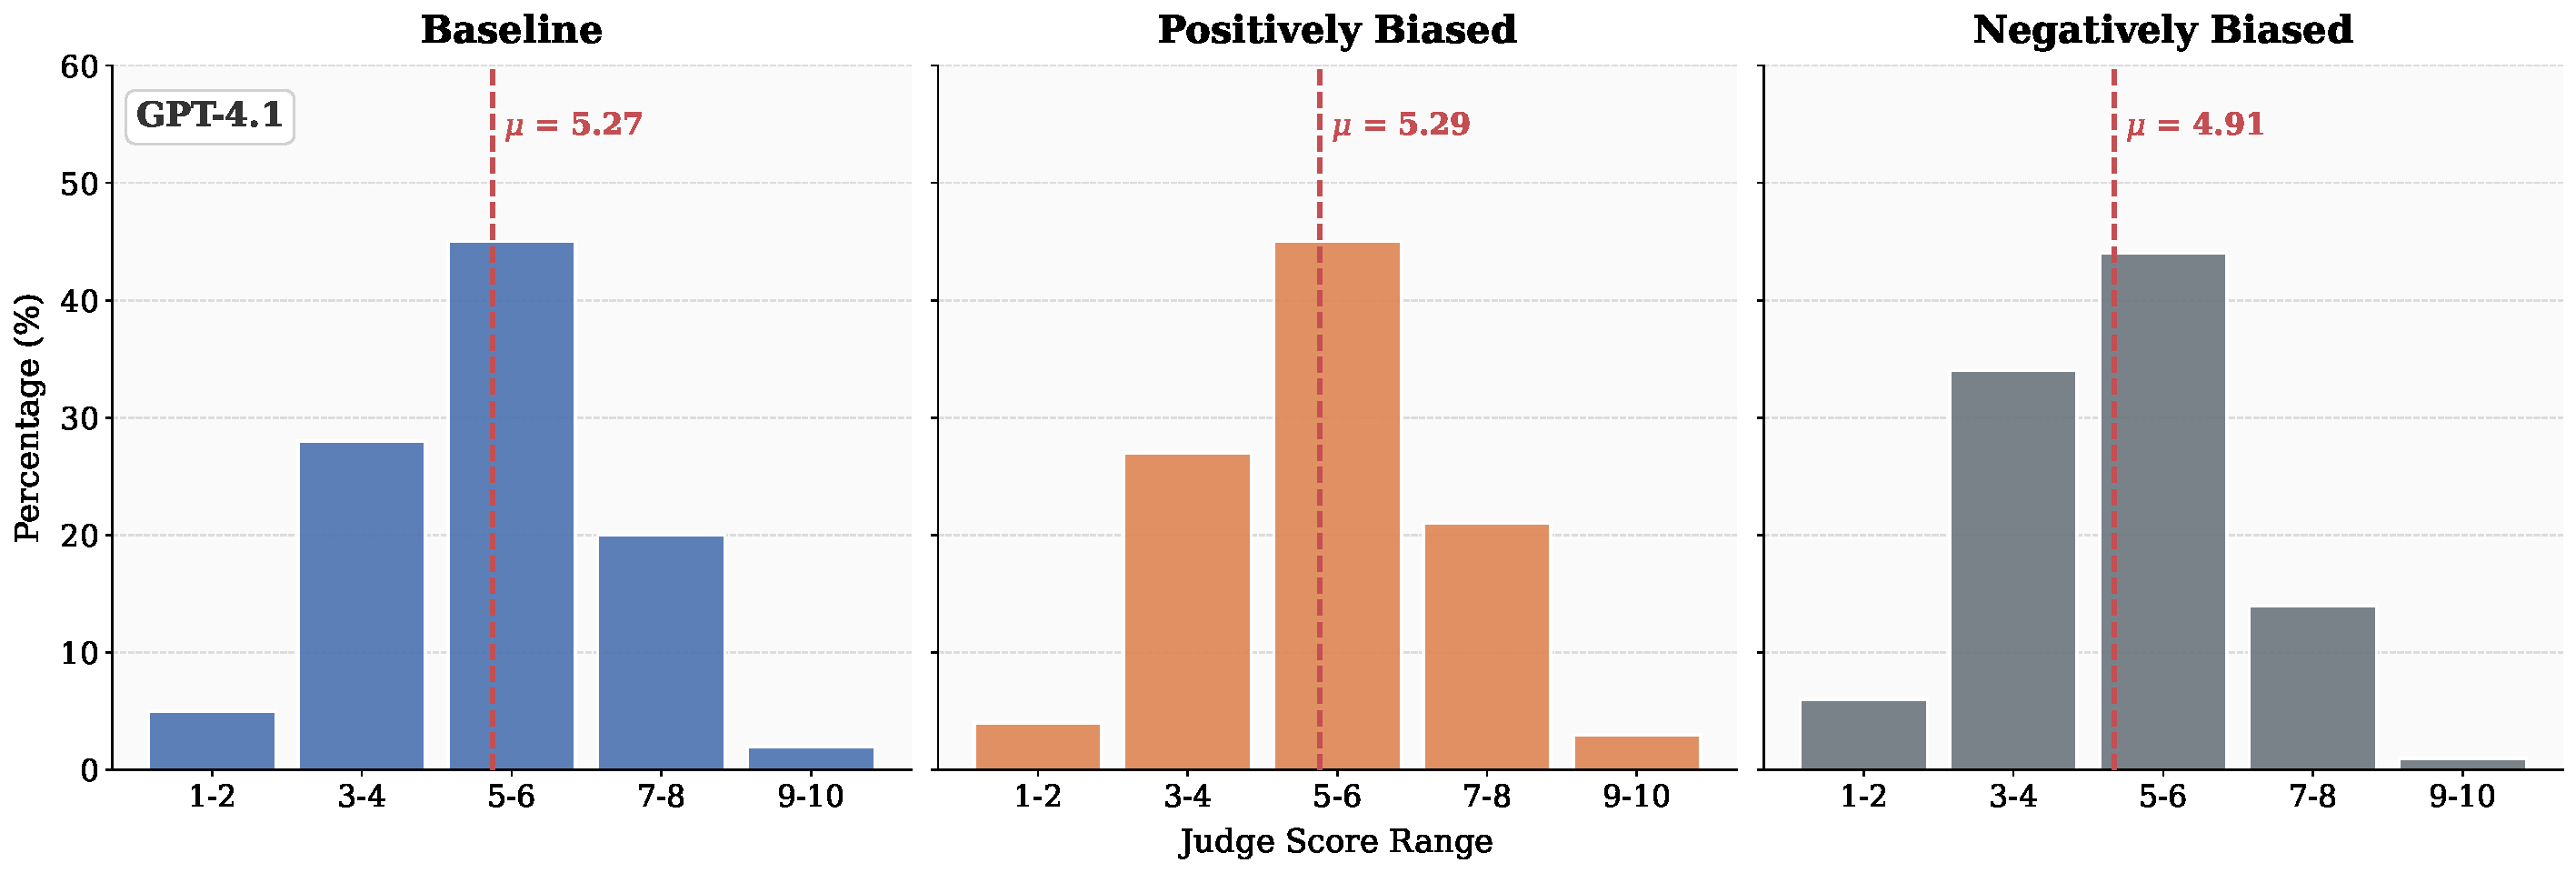
\includegraphics[width=\textwidth]{images/score_distribution_GPT-4.1.pdf}
    \caption{\textsc{GPT-4.1}}
\end{subfigure}
\hfill
\begin{subfigure}[b]{0.48\textwidth}
    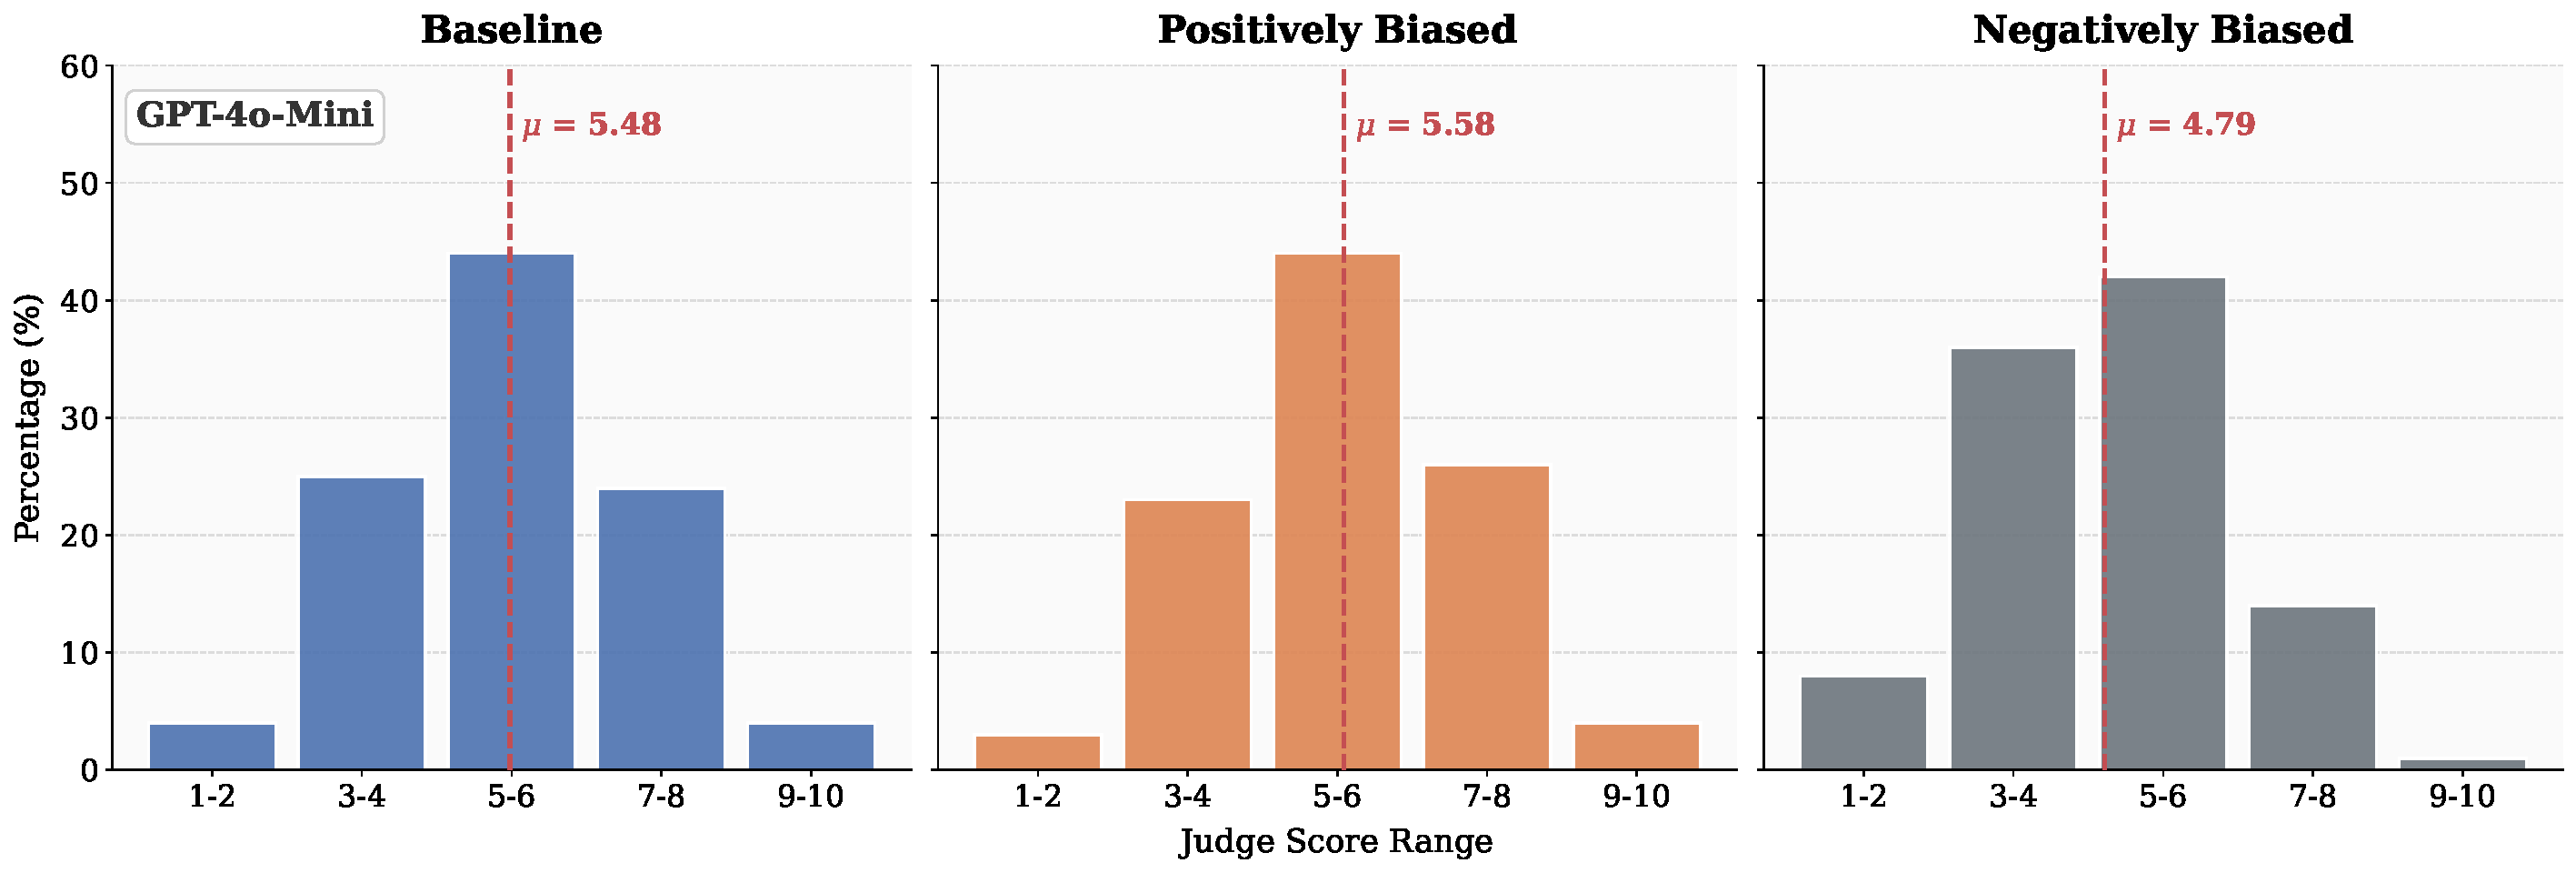
\includegraphics[width=\textwidth]{images/score_distribution_GPT-4o-Mini.pdf}
    \caption{\textsc{GPT-4o-Mini}}
\end{subfigure}
\\[0.5em]
\begin{subfigure}[b]{0.48\textwidth}
    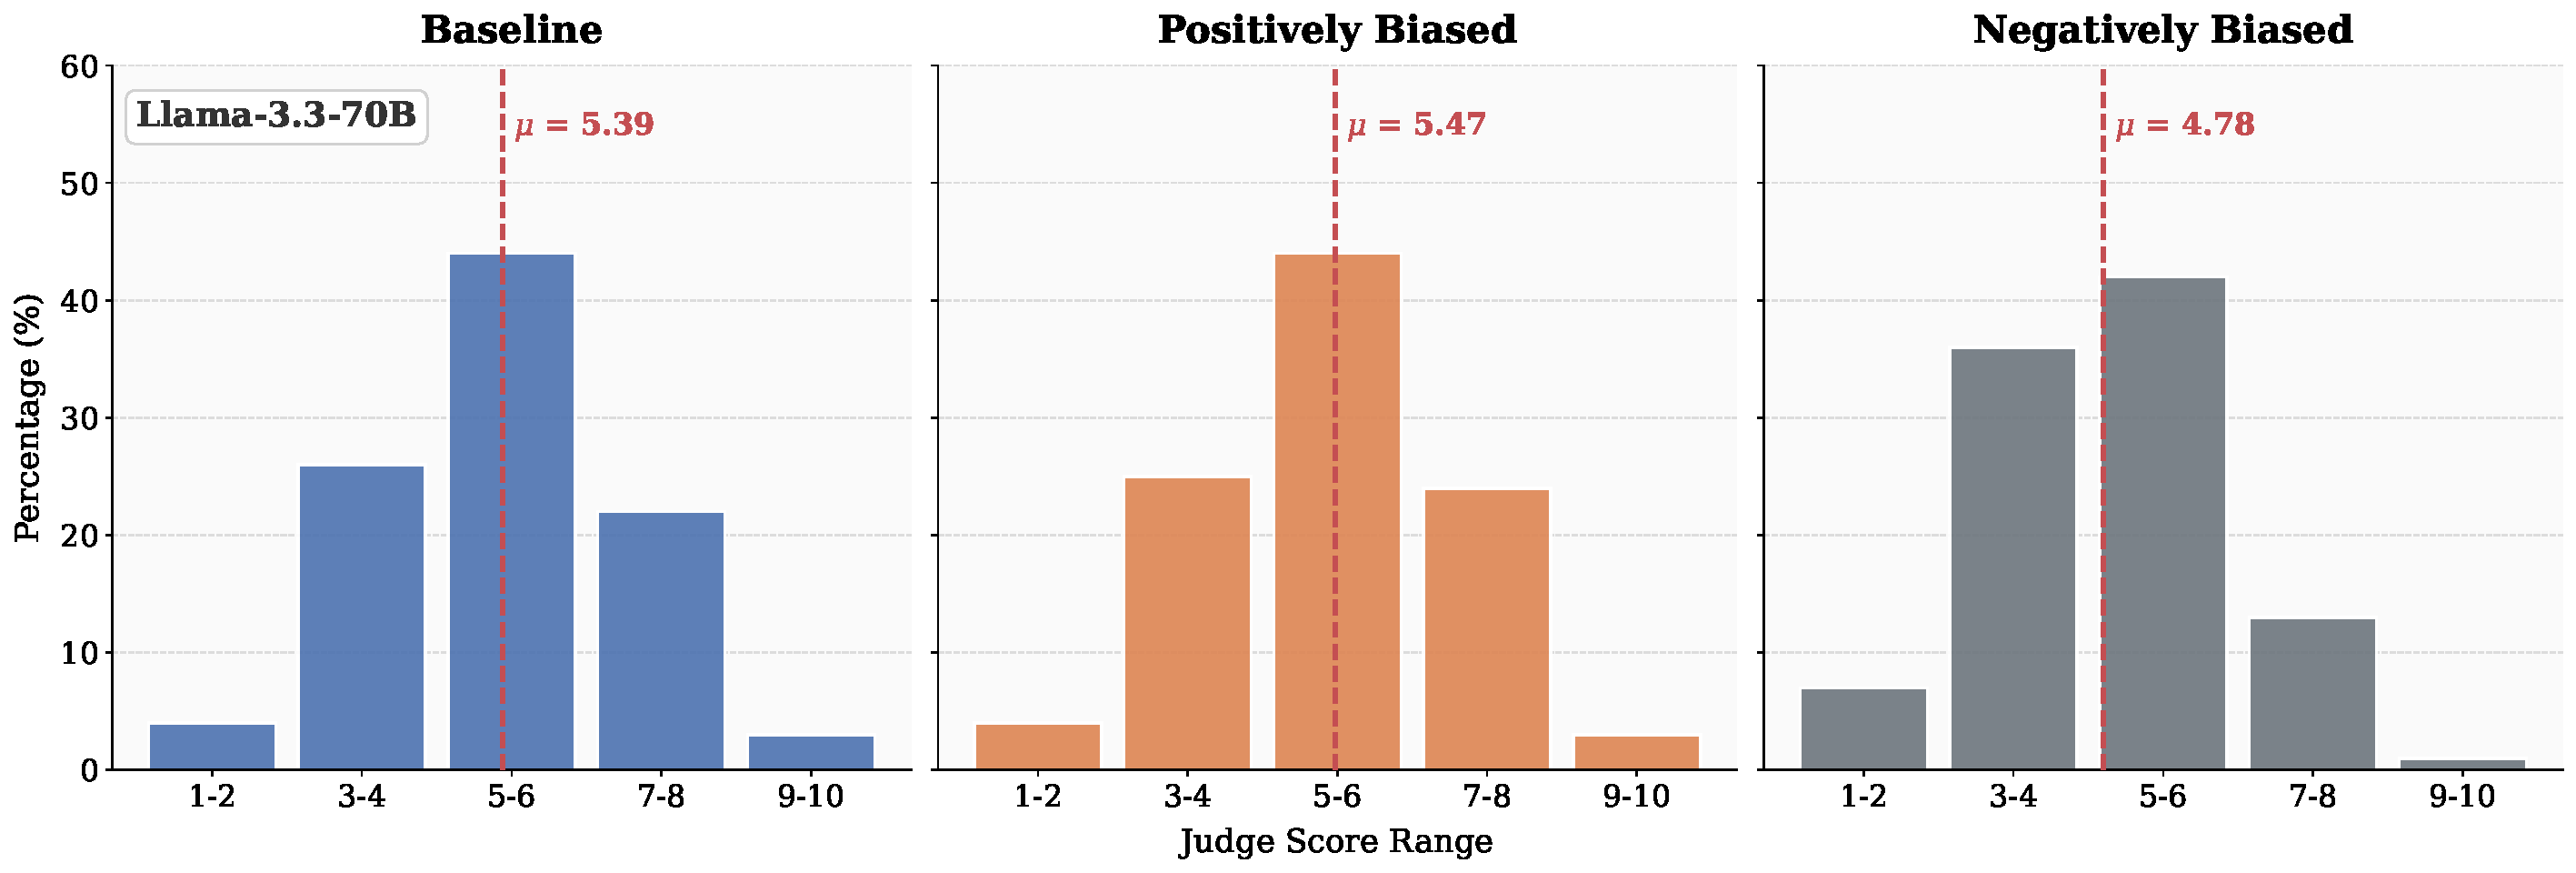
\includegraphics[width=\textwidth]{images/score_distribution_Llama-3.3-70B.pdf}
    \caption{\textsc{Llama-3.3-70B}}
\end{subfigure}
\hfill
\begin{subfigure}[b]{0.48\textwidth}
    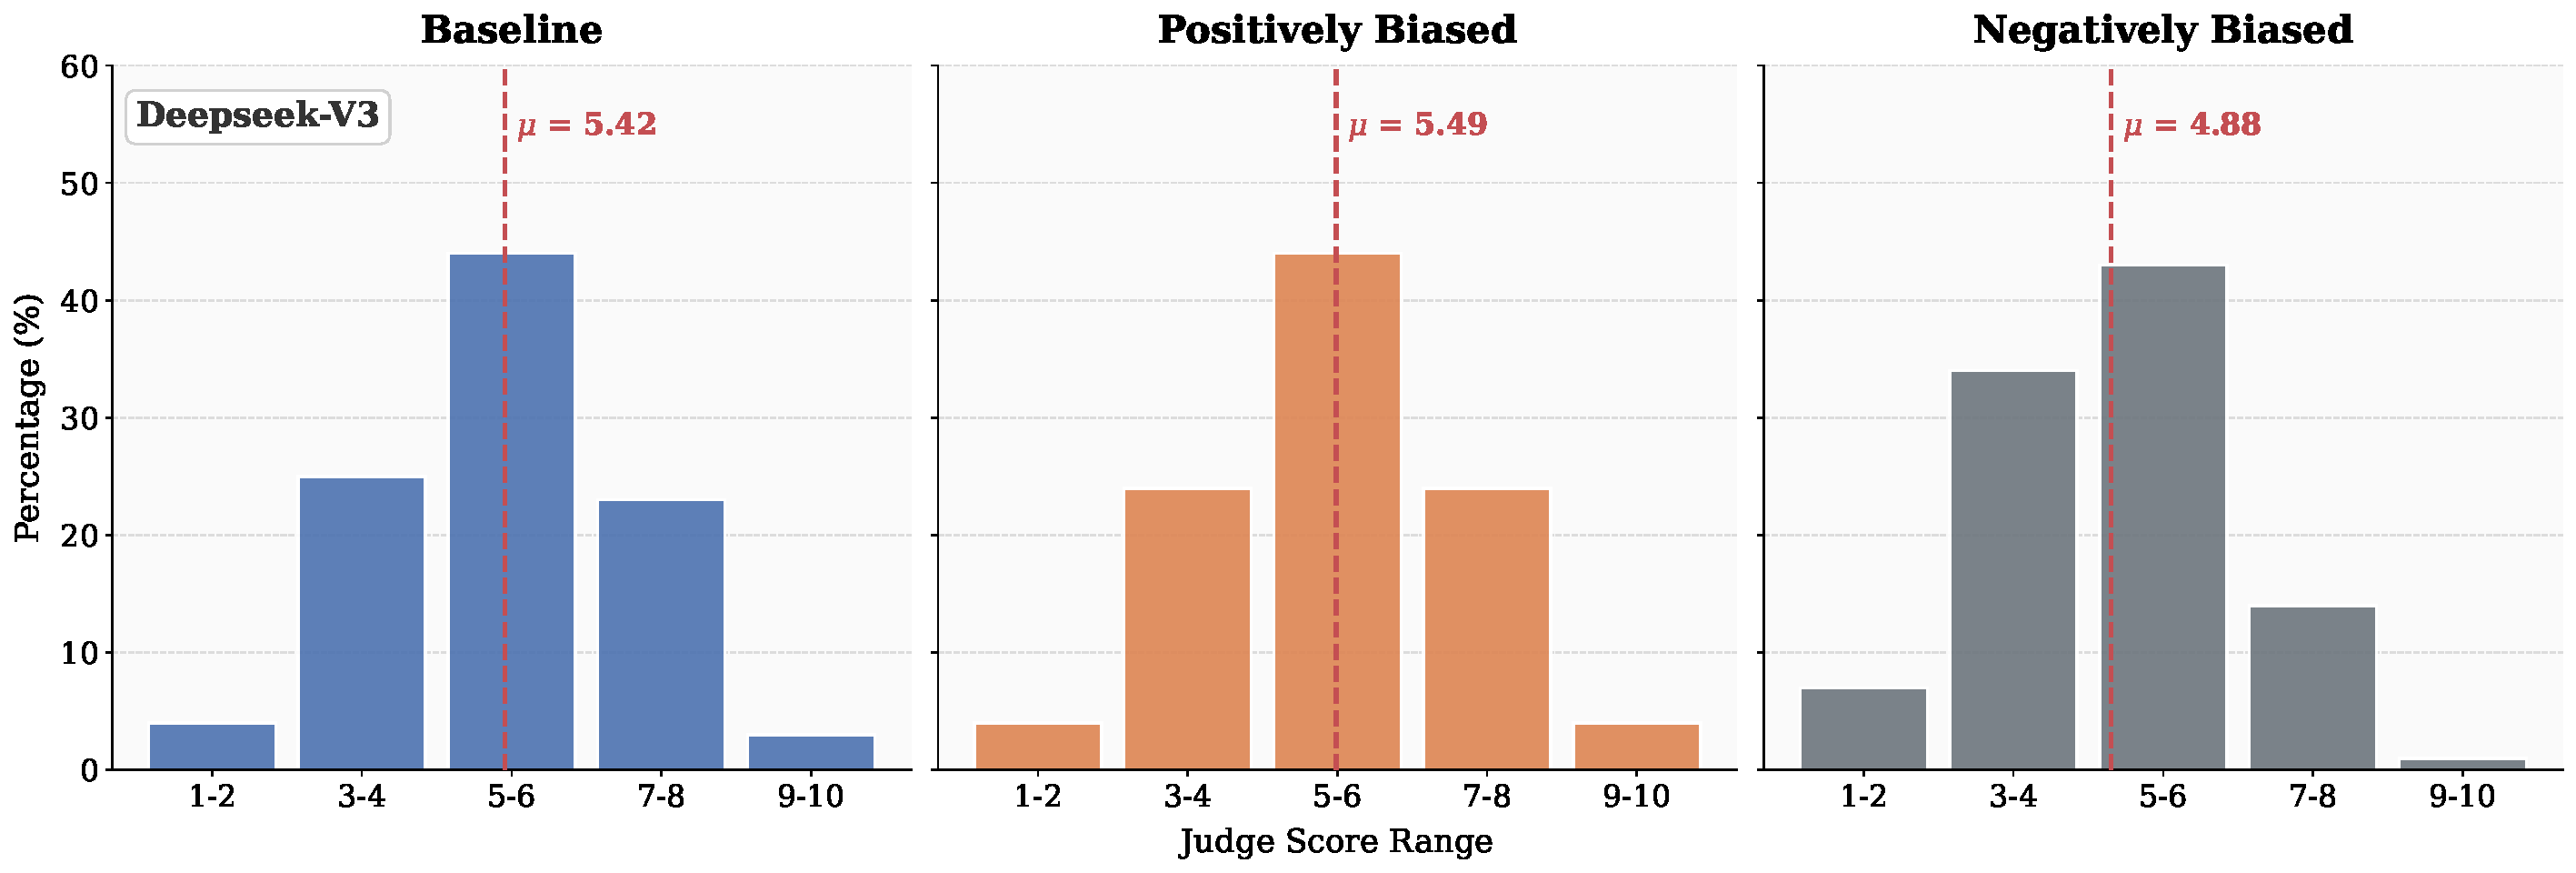
\includegraphics[width=\textwidth]{images/score_distribution_Deepseek-V3.pdf}
    \caption{\textsc{Deepseek-V3}}
\end{subfigure}
\\[0.5em]
\begin{subfigure}[b]{0.48\textwidth}
    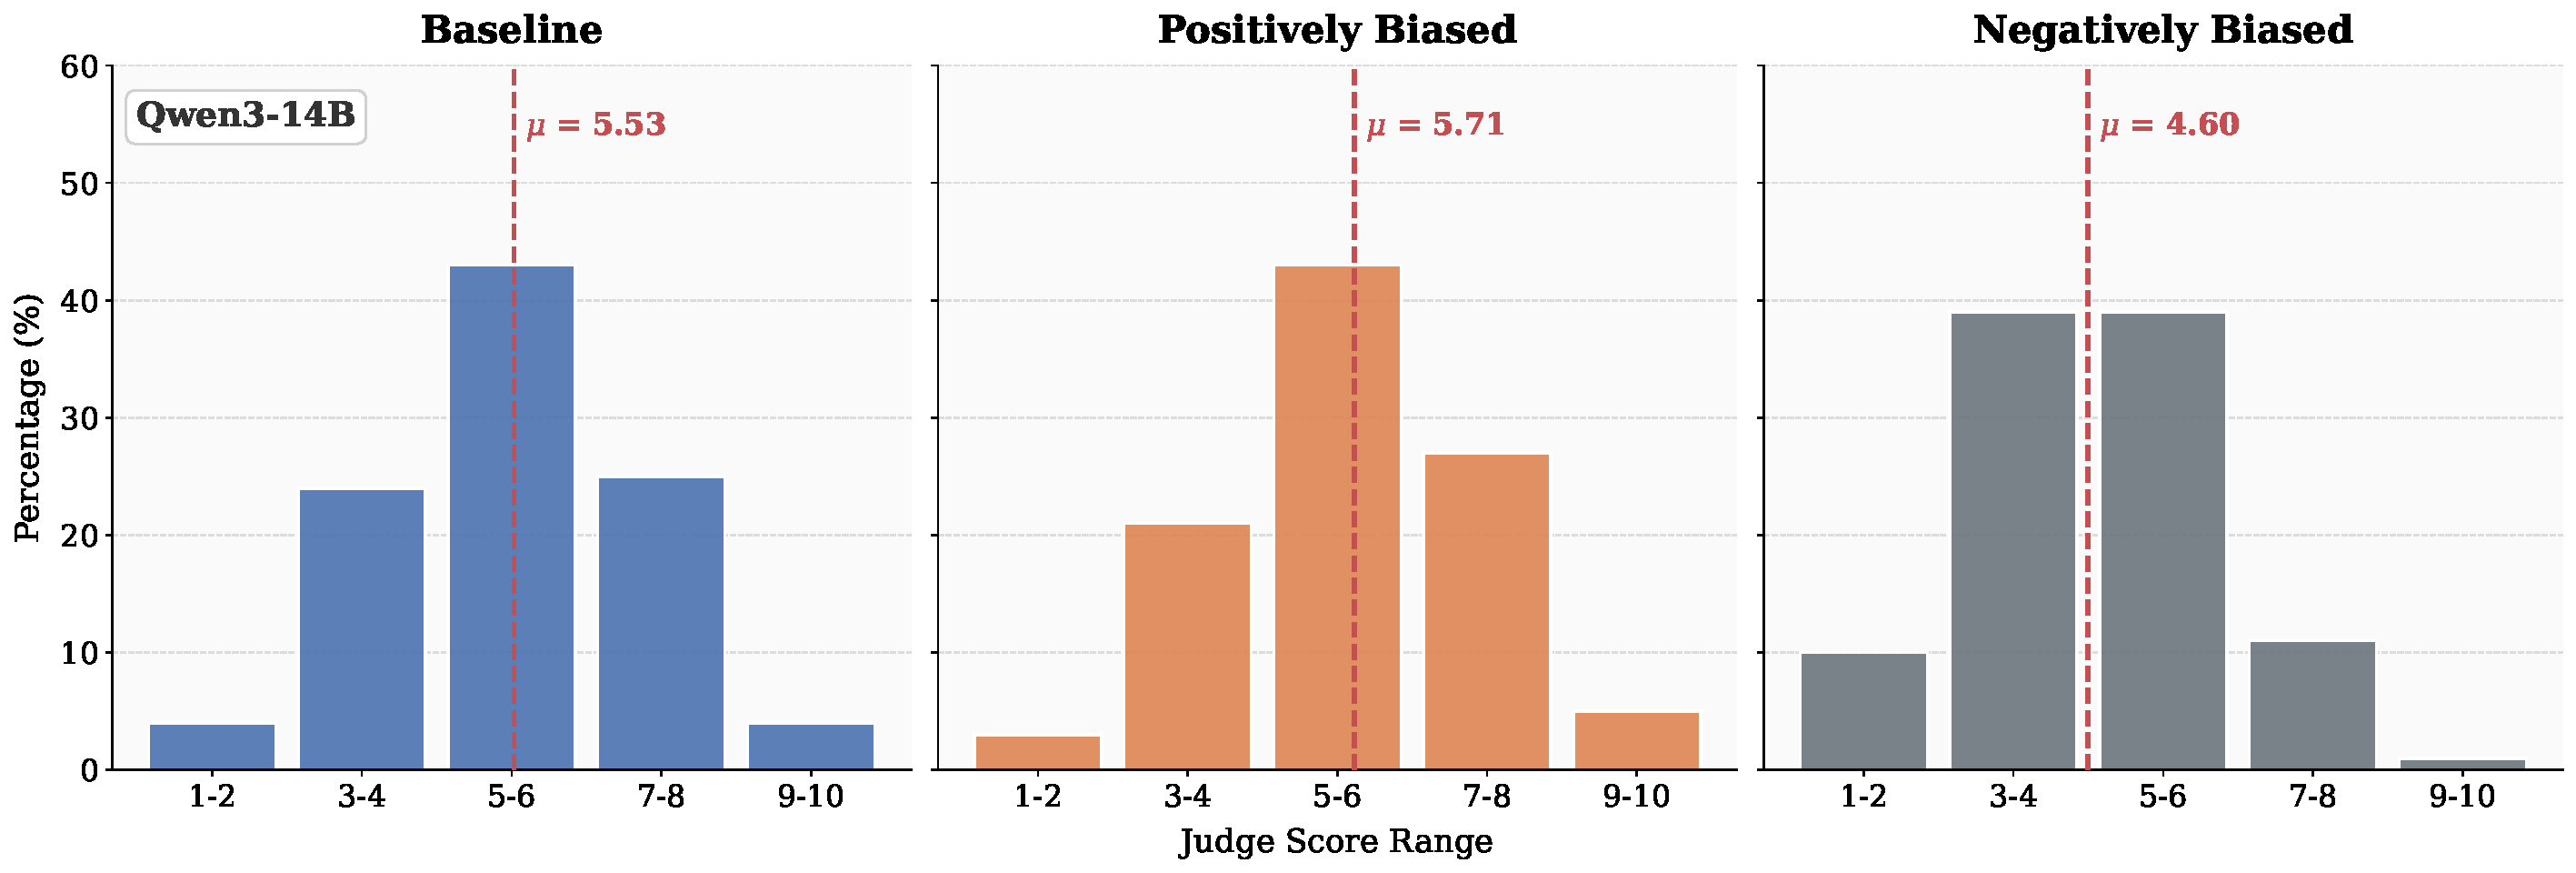
\includegraphics[width=\textwidth]{images/score_distribution_Qwen3-14B.pdf}
    \caption{\textsc{Qwen3-14B}}
\end{subfigure}
\hfill
\begin{subfigure}[b]{0.48\textwidth}
    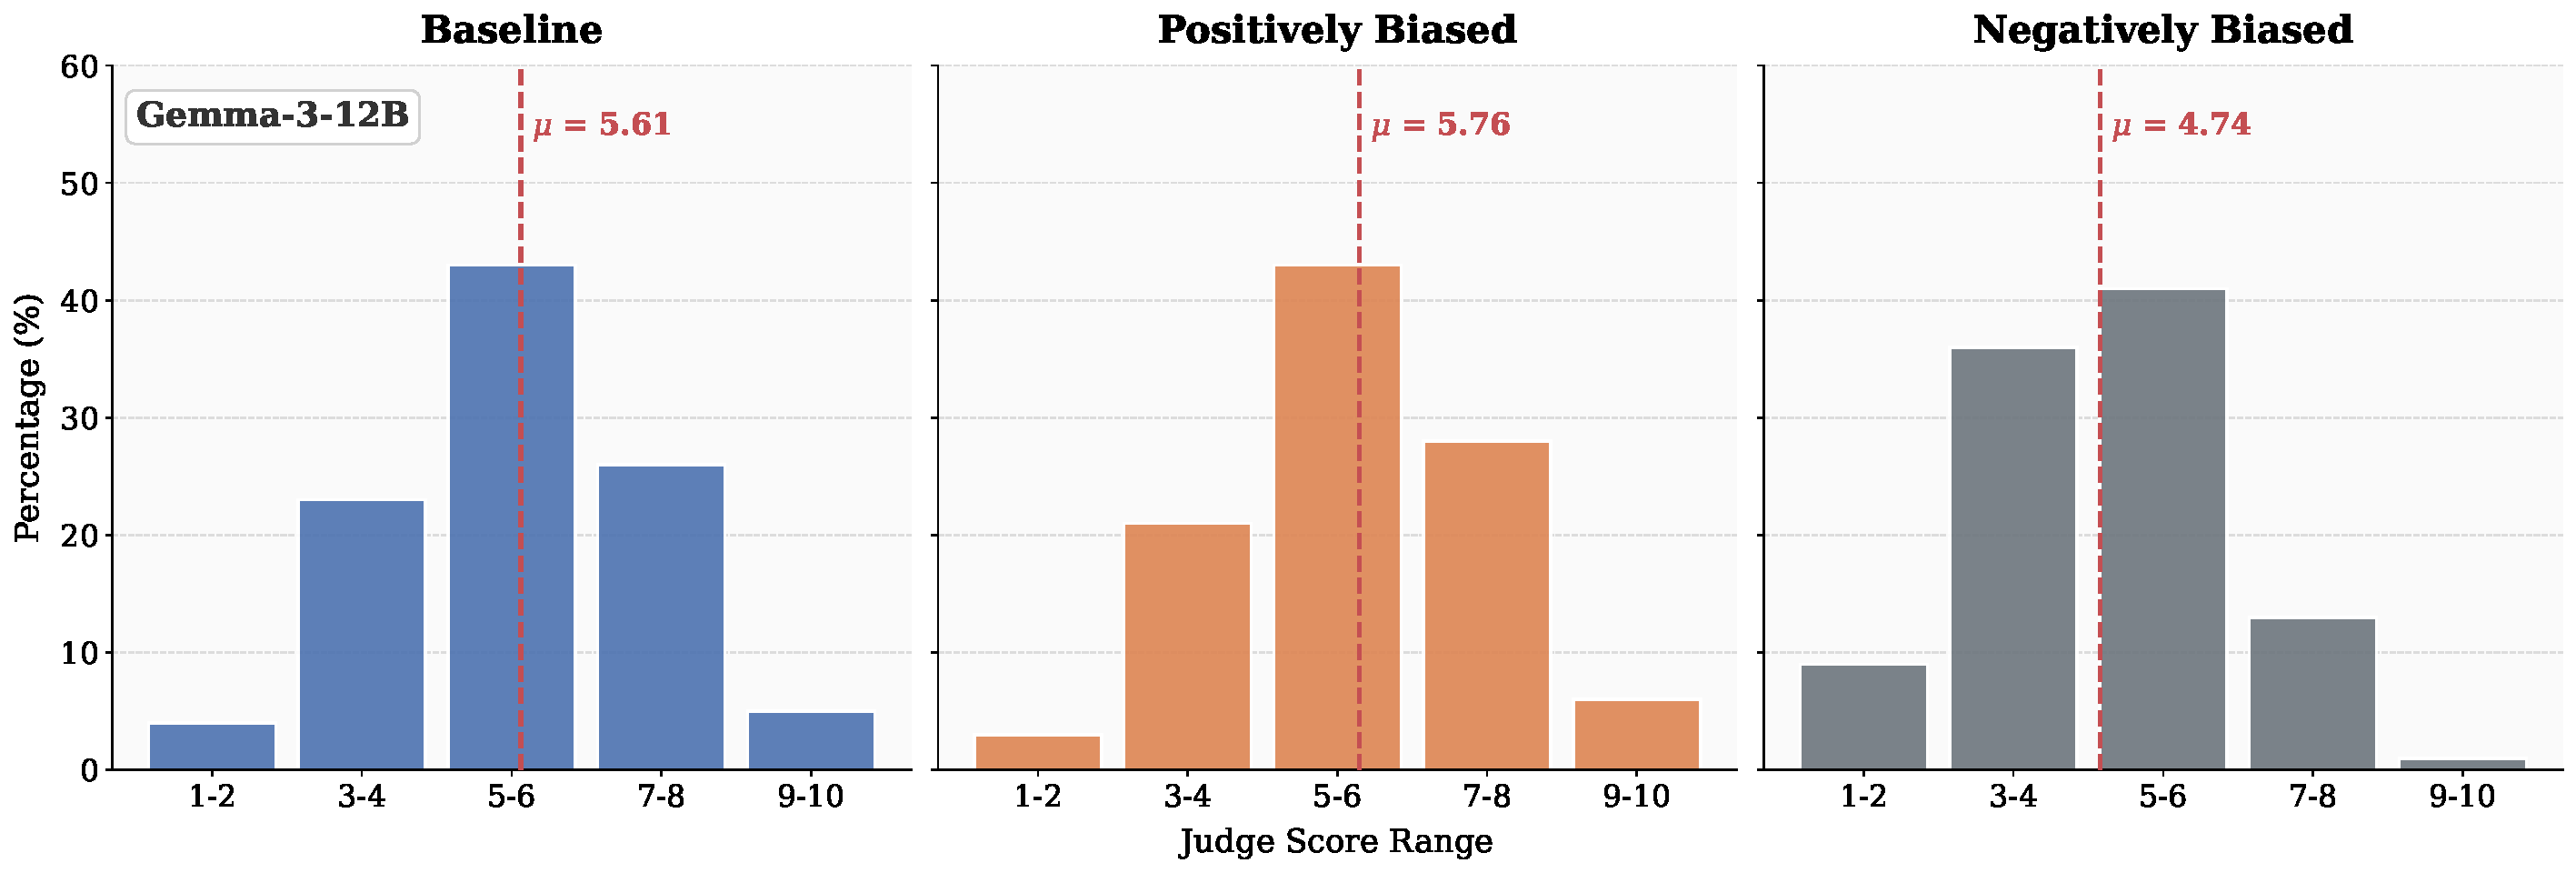
\includegraphics[width=\textwidth]{images/score_distribution_Gemma-3-12B.pdf}
    \caption{\textsc{Gemma-3-12B}}
\end{subfigure}
\caption{Score distributions under the \emph{strict, non-CoT} configuration for all seven judge models (the \textsc{Llama-3.1-8B} distribution is shown in the main text, \Cref{fig:score_dist}). In every case, the negative perturbation distribution (right tail) shifts substantially leftward relative to the baseline, while the positive perturbation distribution remains largely unchanged.}
\label{fig:score_dist_all}
\end{figure*}

\subsection{Geometric Separation Across Models}
\label{app:geometric_replication}

The type-specific geometric separation reported in \Cref{subsec:directional_separation} for \textsc{Llama-3.1-8B} generalizes across architectures. \Cref{fig:mds_qwen,fig:mds_gemma} present MDS projections of per-sample effective bias vectors $\Delta \vec{h}_l$ for Refinement (positive) and Diversity (negative) on \textsc{Qwen3-14B} and \textsc{Gemma-3-12B}, respectively. Both models exhibit the same progressive separation with layer depth, confirming that type-specific geometric signatures are a general property of LLM judge activations rather than an architecture-specific artifact.

\begin{figure*}[t]
\centering
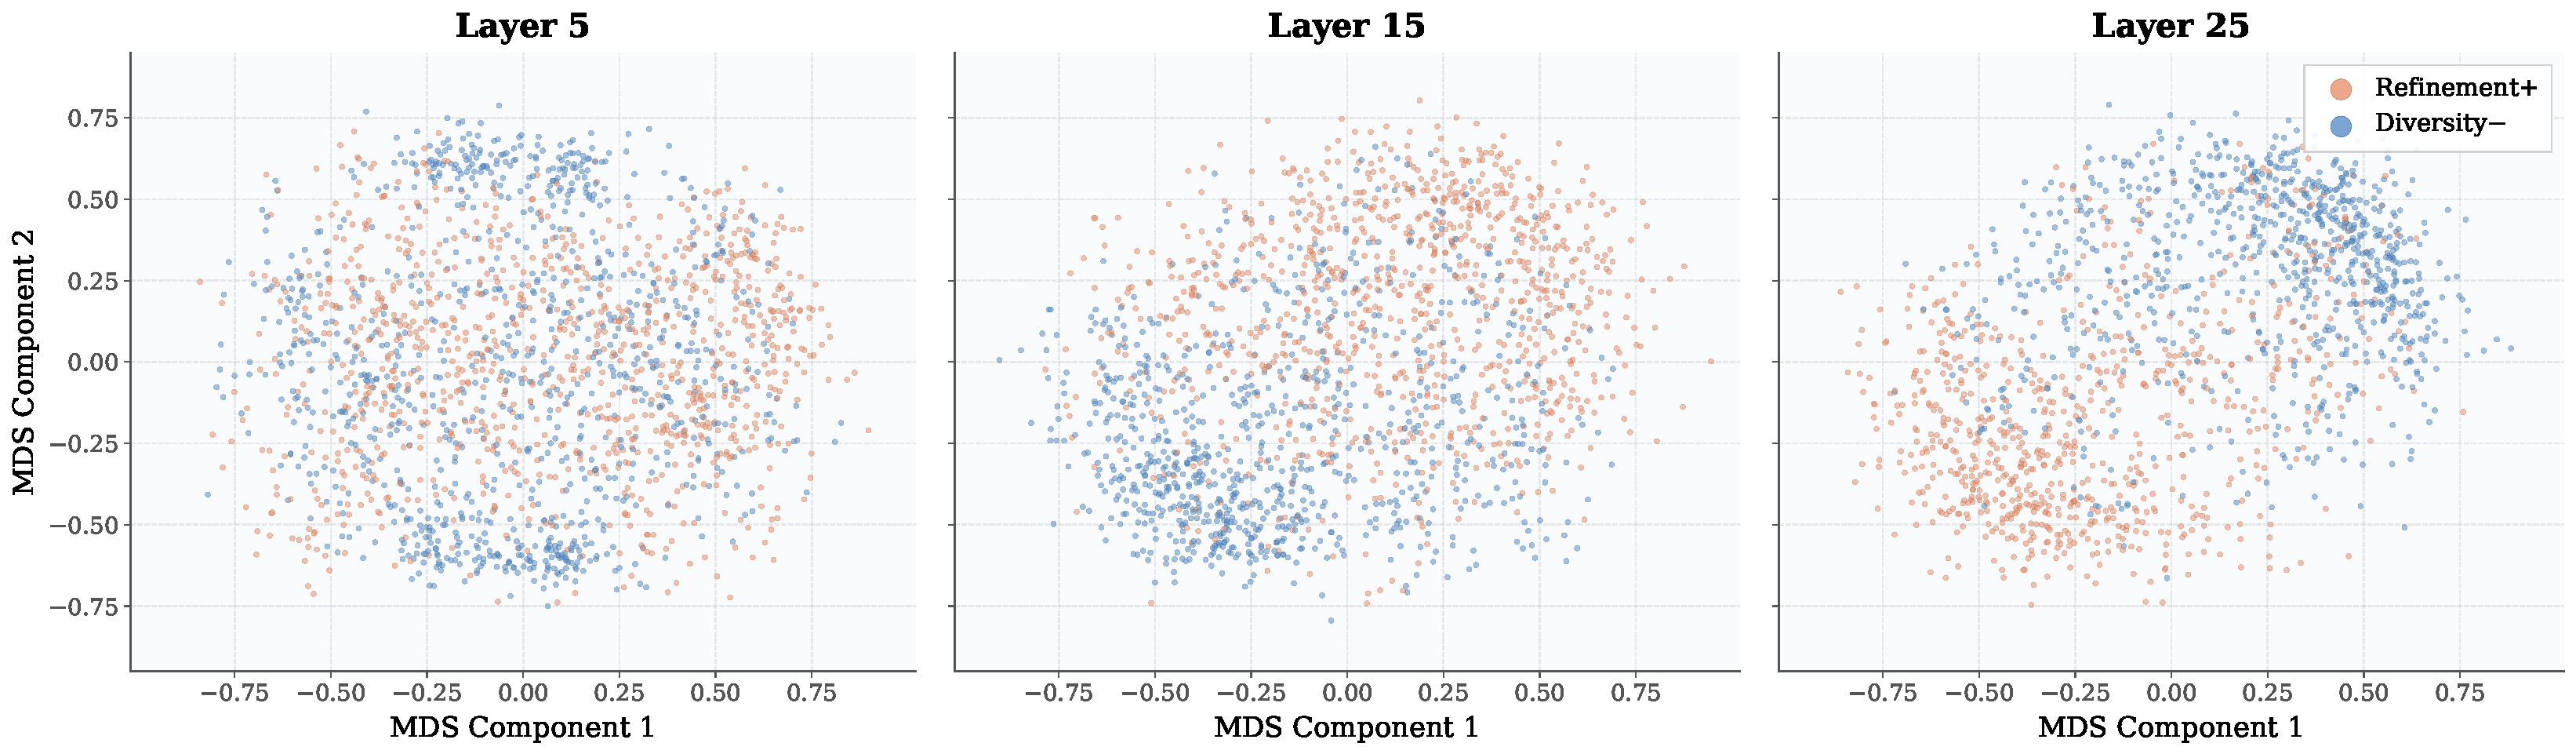
\includegraphics[width=\textwidth]{images/effective_bias_vectors_ref_div_qwen.pdf}
\caption{MDS projection of per-sample effective bias vectors for Refinement+ and Diversity- at layers 5, 15, and 25 of \textsc{Qwen3-14B}. The progressive separation mirrors that observed in \textsc{Llama-3.1-8B} (\Cref{fig:mds_bias_vectors}).}
\label{fig:mds_qwen}
\end{figure*}

\begin{figure*}[t]
\centering
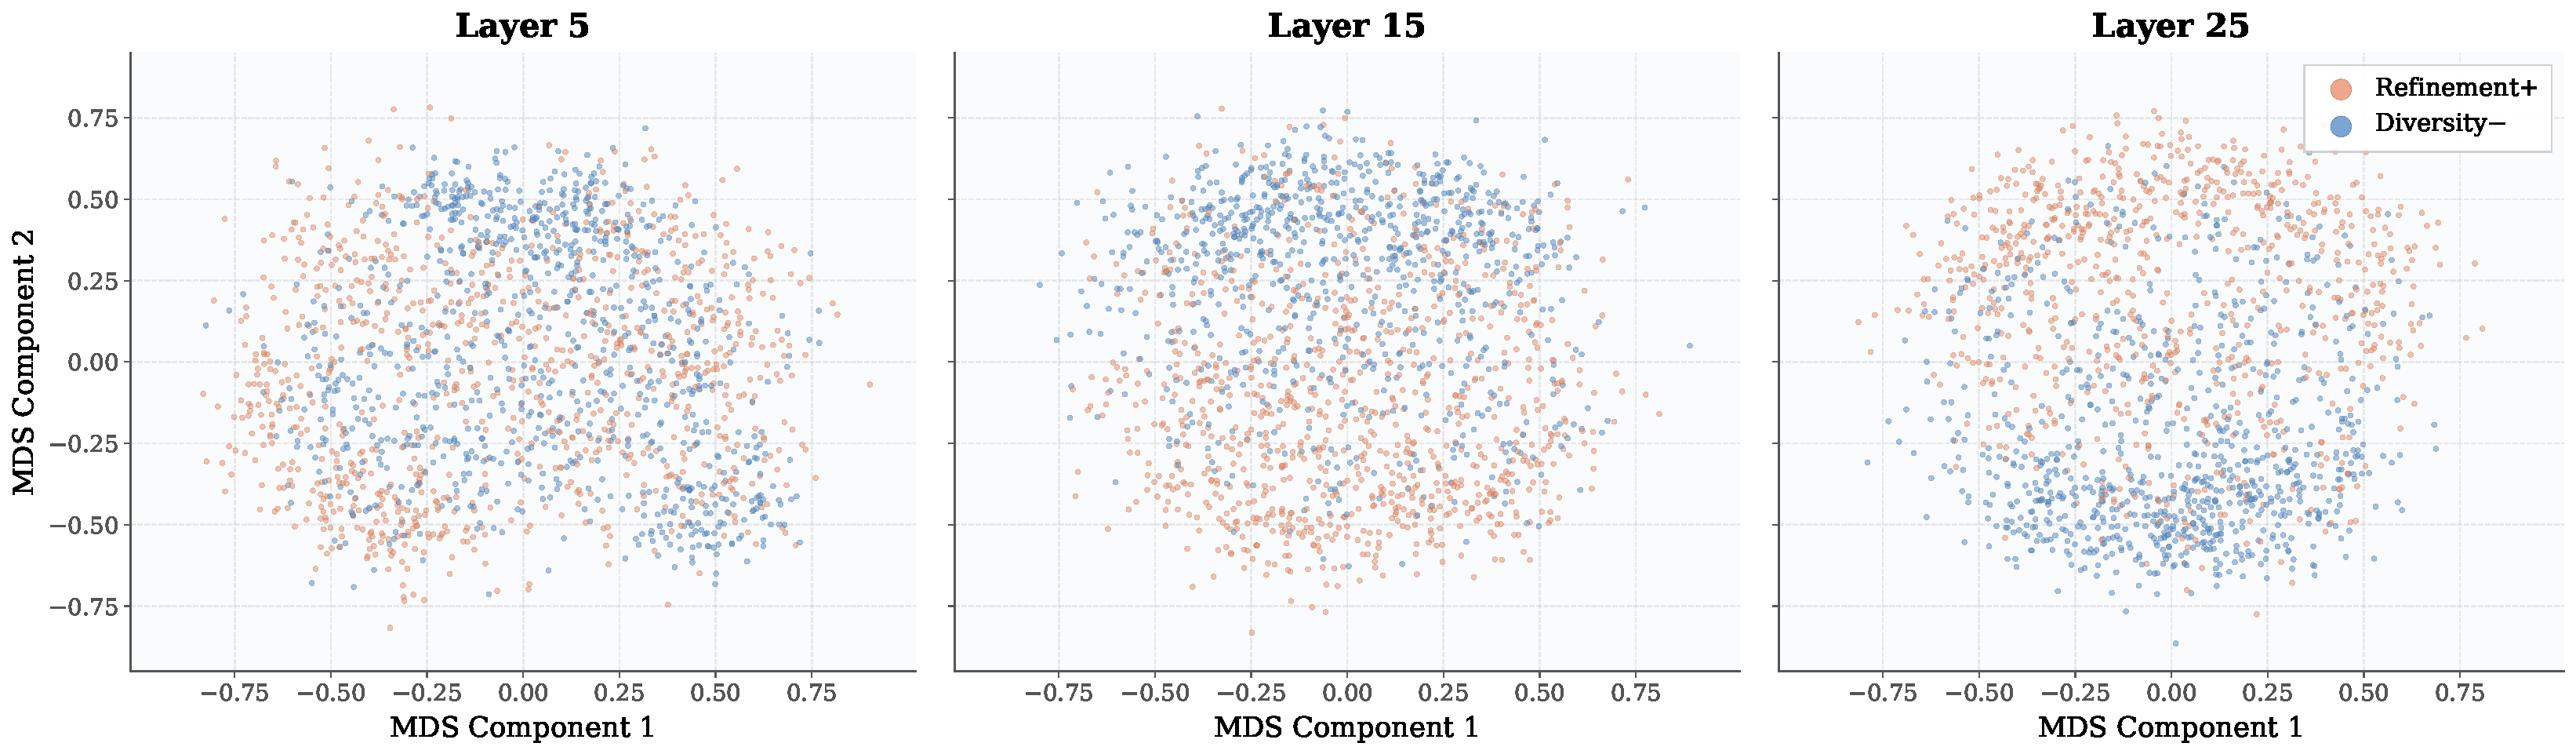
\includegraphics[width=\textwidth]{images/effective_bias_vectors_ref_div_gemma.pdf}
\caption{MDS projection of per-sample effective bias vectors for Refinement+ and Diversity- at layers 5, 15, and 25 of \textsc{Gemma-3-12B}.}
\label{fig:mds_gemma}
\end{figure*}

\section{Complete Attack Results}
\label{app:attack_full}

This appendix provides the full materials supporting \Cref{subsec:causal}: the headline attack/defense summary (\Cref{tab:steering_summary}), the bias-vector candidate analysis (\Cref{app:vector_analysis}), the two-stage $\alpha$-optimization algorithm in pseudocode (\Cref{app:alpha_algo}), the empirical monotonicity of our three optimization metrics (\Cref{app:alpha_monotone}), and per-layer, per-method attack tables for the six bias types covering the strongest negative and positive perturbations (\Cref{app:attack_tables}).

\begin{table*}[t]
\centering
\small
\setlength{\tabcolsep}{6pt}
\caption{Best activation steering for attack and defense on \textsc{Llama-3.1-8B}, test set. ``Atk-$W_1$'' is shift magnitude (higher = stronger attack); ``Def-$W_1\!\downarrow$'' is the fractional reduction in pre-defense Wasserstein distance (higher = better recovery); $\rho_S$ is Spearman rank correlation with baseline. Activation interventions Pareto-dominate text-level baselines on both tasks. Full per-layer, per-method tables in \Cref{app:attack_tables,app:defense_full}.}
\label{tab:steering_summary}
\begin{tabular}{l l cccc}
\toprule
\textbf{Bias} & \textbf{Method} & \textbf{Atk-}$W_1$\,$\uparrow$ & $\rho_S$\,$\uparrow$ & \textbf{Def-}$W_1\!\downarrow$\,$\uparrow$ & $\rho_S$\,$\uparrow$ \\
\midrule
\multirow{2}{*}{Auth.$-$} & Text & 0.78 & 0.70 & 0.11 & 0.74 \\
& \textbf{Cls.} & \textbf{1.62} & \textbf{0.78} & \textbf{0.62} & \textbf{0.81} \\
\midrule
\multirow{2}{*}{Bandw.$-$} & Text & 1.66 & 0.51 & 0.09 & 0.56 \\
& \textbf{PCA} & \textbf{3.43} & \textbf{0.58} & \textbf{0.61} & \textbf{0.67} \\
\midrule
\multirow{2}{*}{Refin.$-$} & Text & 0.59 & 0.76 & 0.15 & 0.77 \\
& \textbf{PCA/Cls.}$^{\dagger}$ & \textbf{1.13} & \textbf{0.80} & \textbf{0.52} & \textbf{0.83} \\
\bottomrule
\end{tabular}
\\[-0.2em]
{\scriptsize $^{\dagger}$Attack: PCA; Defense: Classifier.}
\end{table*}

\subsection{Bias-Vector Candidate Analysis}
\label{app:vector_analysis}

We extracted six candidate bias vectors---three \emph{directional-change} (Mean, Geometric Median, PCA) and three \emph{discriminative-boundary} (LDA, Classifier, SVM)---from the training set of \textsc{Llama-3.1-8B} for each bias type. \Cref{tab:vector_cosine} reports the pairwise cosine similarity averaged across Authority$-$, Bandwagon$-$, and Refinement$-$ at layer 25.

\begin{table*}[t]
\centering
\small
\caption{Mean pairwise cosine similarity between the six candidate bias vectors at layer 25 of \textsc{Llama-3.1-8B}, averaged across three negative bias types. Within each family (shaded blocks on the diagonal), agreement is high; cross-family agreement is noticeably lower, motivating our three-representative selection.}
\label{tab:vector_cosine}
\setlength{\tabcolsep}{6pt}
\begin{tabular}{l cccccc}
\toprule
 & Mean & Geom. Med. & PCA & LDA & Classifier & SVM \\
\midrule
Mean & -- & 0.98 & 0.94 & 0.58 & 0.62 & 0.59 \\
Geom. Median & 0.98 & -- & 0.93 & 0.61 & 0.65 & 0.62 \\
PCA & 0.94 & 0.93 & -- & 0.55 & 0.60 & 0.57 \\
\midrule
LDA & 0.58 & 0.61 & 0.55 & -- & 0.95 & 0.91 \\
Classifier & 0.62 & 0.65 & 0.60 & 0.95 & -- & 0.94 \\
SVM & 0.59 & 0.62 & 0.57 & 0.91 & 0.94 & -- \\
\bottomrule
\end{tabular}
\end{table*}

The block structure confirms the qualitative description in the main text: within-family cosine similarity is $\geq 0.91$, while cross-family cosine similarity sits in $[0.55, 0.65]$---tight enough that the two families share a coarse direction, but loose enough to suggest they capture distinct notions of bias direction. We therefore keep three representatives that span this geometry: \emph{Geometric Median} (robust directional summary), \emph{PCA} (principal directional axis), and the \emph{Classifier} vector (a discriminative-family stand-in for LDA and SVM, which agree with it at $\cos \geq 0.94$).

\subsection{Two-Stage $\alpha$-Optimization Algorithm}
\label{app:alpha_algo}

\Cref{alg:alpha_search} pinpoints the optimal intervention strength under the feasibility set $\mathcal{F}$ defined in \Cref{eq:alpha_obj}. Stage 1 exploits the monotonicity of $V(\alpha)$ and $\rho_S(\alpha)$ to locate the boundary $\alpha_{\text{bd}}$ in $\mathcal{O}(\log \alpha_{\max} + \log(1/\epsilon))$ evaluations. Stage 2 refines by simulated annealing within a small neighborhood of $\alpha_{\text{bd}}$, which is necessary because the integer-score output makes $W_1(\alpha)$ piecewise-constant and induces local plateaus that a pure greedy search would get stuck on.

\begin{algorithm}[h!]
\caption{Two-stage search for optimal activation-steering strength.}
\label{alg:alpha_search}
\begin{algorithmic}[1]
\REQUIRE Bias vector $\vec{v}_{\text{bias}}^{(l)}$, initial step $\alpha_0 > 0$, tolerance $\epsilon$, neighborhood $\Delta$, SA schedule $(T_0, T_{\min}, \gamma)$
\ENSURE Optimal strength $\alpha^{*} \in \mathcal{F}$ maximizing $W_1$

\STATE \textcolor{gray}{\emph{// Stage 1: Boundary identification}}
\STATE $\alpha_{\text{lo}} \gets 0$, $\alpha_{\text{hi}} \gets \alpha_0$
\WHILE{$\alpha_{\text{hi}} \in \mathcal{F}$}
    \STATE $\alpha_{\text{lo}} \gets \alpha_{\text{hi}}$, $\alpha_{\text{hi}} \gets 2\alpha_{\text{hi}}$ \COMMENT{exponential expansion}
\ENDWHILE
\WHILE{$\alpha_{\text{hi}} - \alpha_{\text{lo}} > \epsilon$}
    \STATE $\alpha_{\text{mid}} \gets (\alpha_{\text{lo}} + \alpha_{\text{hi}})/2$
    \IF{$\alpha_{\text{mid}} \in \mathcal{F}$}
        \STATE $\alpha_{\text{lo}} \gets \alpha_{\text{mid}}$
    \ELSE
        \STATE $\alpha_{\text{hi}} \gets \alpha_{\text{mid}}$
    \ENDIF
\ENDWHILE
\STATE $\alpha_{\text{bd}} \gets \alpha_{\text{lo}}$

\STATE \textcolor{gray}{\emph{// Stage 2: Simulated-annealing refinement}}
\STATE $\alpha_{\text{best}} \gets \alpha_{\text{bd}}$, $W^{*} \gets W_1(\alpha_{\text{bd}})$, $T \gets T_0$
\WHILE{$T > T_{\min}$}
    \STATE Sample $\alpha' \sim \mathcal{U}(\alpha_{\text{bd}} - \Delta,\, \alpha_{\text{bd}})$
    \STATE $E' \gets -W_1(\alpha') + M \cdot \mathbb{1}[\alpha' \notin \mathcal{F}]$
    \IF{$E' < -W^{*}$ \OR $\exp((-W^{*} - E')/T) > u$, $u \sim \mathcal{U}(0,1)$}
        \STATE $\alpha_{\text{best}} \gets \alpha'$, $W^{*} \gets -E'$
    \ENDIF
    \STATE $T \gets \gamma T$
\ENDWHILE
\RETURN $\alpha_{\text{best}}$
\end{algorithmic}
\end{algorithm}

\subsection{Monotonicity of the Optimization Metrics}
\label{app:alpha_monotone}

\Cref{tab:alpha_monotone} illustrates the empirical monotonicity that underpins Stage 1 of the algorithm: $W_1(\alpha)$ is monotonically non-decreasing while $V(\alpha)$ and $\rho_S(\alpha)$ are monotonically non-increasing in $|\alpha|$, so the feasible boundary $\alpha_{\text{bd}}$ is well-defined. The table aggregates over all $(l, \vec{v}_{\text{bias}}, \text{bias type})$ triples and reports the fraction that exhibit strict monotonicity along each axis.

\begin{table}[h!]
\centering
\small
\setlength{\tabcolsep}{3pt}
\caption{Empirical monotonicity of the three optimization metrics with respect to $|\alpha|$ across all configurations on \textsc{Llama-3.1-8B}. Each row reports the fraction of $(l, \vec{v}_{\text{bias}}, \text{bias type})$ triples that exhibit strictly monotone behavior along the stated direction.}
\label{tab:alpha_monotone}
\begin{tabular}{l ccc}
\toprule
\textbf{Metric} & \textbf{Mono.} & \textbf{Non-mono.} & \textbf{Direction} \\
\midrule
$W_1(\alpha)$ (efficacy) & 97\% & 3\% & non-decr. \\
$V(\alpha)$ (validity) & 99\% & 1\% & non-incr. \\
$\rho_S(\alpha)$ (Spearman) & 93\% & 7\% & non-incr. \\
\bottomrule
\end{tabular}
\end{table}

\subsection{Per-Layer, Per-Method Attack Tables}
\label{app:attack_tables}

We report the complete per-layer attack results for \textsc{Llama-3.1-8B} on the test set across six bias types---the five strongest negative biases (Authority$-$, Bandwagon$-$, Diversity$-$, Refinement$-$, Verbosity$-$) and the strongest positive bias (Refinement$+$)---using our three retained vector methods (Geometric Median, PCA, Classifier) plus the text-attack baseline. Each row is the layer-optimal $\alpha^{*}$ selected by \Cref{alg:alpha_search} on the development set; we then evaluate on the test split.

\begin{table*}[h!]
\centering
\small
\setlength{\tabcolsep}{6pt}
\caption{Per-bias attack performance on \textsc{Llama-3.1-8B}, test set. Each block reports the four methods (text-attack baseline plus three activation methods); best per-metric values within each block in bold. Refinement$+$ is the only positive bias in the attack suite; its activation push is in the score-up direction.}
\label{tab:attack_per_bias}
\begin{tabular}{l l c c c c c}
\toprule
\textbf{Bias} & \textbf{Method} & $W_1 \uparrow$ & $\rho_S \uparrow$ & \textbf{Valid.} & \textbf{Layer} & $\alpha^{*}$ \\
\midrule
\multirow{4}{*}{Authority$-$}
 & Text Atk (baseline) & 0.780 & 0.696 & 100\% & -- & -- \\
 & Geometric Median & 1.214 & 0.716 & 93.8\% & 31 & 23.84 \\
 & PCA & 0.840 & 0.750 & 100\% & 15 & 8.94 \\
 & Classifier & \textbf{1.618} & \textbf{0.780} & 94.8\% & 30 & 62.36 \\
\midrule
\multirow{4}{*}{Bandwagon$-$}
 & Text Atk (baseline) & 1.664 & 0.514 & 100\% & -- & -- \\
 & Geometric Median & 1.333 & \textbf{0.708} & 99.3\% & 7 & 5.00 \\
 & PCA & \textbf{3.426} & 0.584 & 94.8\% & 31 & 75.75 \\
 & Classifier & 1.744 & 0.627 & 100\% & 15 & 5.70 \\
\midrule
\multirow{4}{*}{Refinement$-$}
 & Text Atk (baseline) & 0.594 & 0.757 & 100\% & -- & -- \\
 & Geometric Median & 0.485 & 0.805 & 100\% & 7 & 2.19 \\
 & PCA & \textbf{1.132} & 0.800 & 100\% & 31 & 35.53 \\
 & Classifier & 0.799 & 0.803 & 100\% & 18 & 7.70 \\
\midrule
\multirow{4}{*}{Diversity$-$}
 & Text Atk (baseline) & 1.452 & 0.610 & 100\% & -- & -- \\
 & Geometric Median & 1.892 & \textbf{0.732} & 98.2\% & 30 & 22.50 \\
 & PCA & \textbf{2.654} & 0.643 & 96.1\% & 31 & 58.20 \\
 & Classifier & 2.345 & 0.689 & 98.5\% & 28 & 33.00 \\
\midrule
\multirow{4}{*}{Verbosity$-$}
 & Text Atk (baseline) & 0.612 & 0.723 & 100\% & -- & -- \\
 & Geometric Median & 0.875 & \textbf{0.785} & 99.5\% & 25 & 12.40 \\
 & PCA & \textbf{1.456} & 0.701 & 95.8\% & 31 & 53.00 \\
 & Classifier & 1.122 & 0.748 & 98.0\% & 18 & 8.50 \\
\midrule
\multirow{4}{*}{Refinement$+$}
 & Text Atk (baseline) & 0.382 & 0.812 & 100\% & -- & -- \\
 & Geometric Median & 0.541 & \textbf{0.825} & 100\% & 22 & 8.80 \\
 & PCA & \textbf{0.852} & 0.788 & 98.6\% & 31 & 18.40 \\
 & Classifier & 0.673 & 0.815 & 100\% & 25 & 12.00 \\
\bottomrule
\end{tabular}
\end{table*}

\paragraph{Cross-bias observations.}
\Cref{tab:attack_per_bias} surfaces four robust patterns, matching our summary in the main text. \emph{(1) Heterogeneous optimal strength}: $\alpha^{*}$ varies from 2.19 (Refinement$-$, Geom. Med., layer 7) to 75.75 (Bandwagon$-$, PCA, layer 31)---more than an order of magnitude---so a universal attack strength is infeasible. \emph{(2) Depth-dependent strength}: the optimal layer for each method is concentrated at layer $\geq 15$, reflecting that middle-to-late layers carry the cleanest bias direction (consistent with \Cref{tab:layerwise}); positive Refinement is the lone exception, peaking in the mid-layers. \emph{(3) Method complementarity}: Classifier vectors dominate the score-shift axis for Authority$-$; PCA dominates for Bandwagon$-$, Diversity$-$, Refinement$-$, Verbosity$-$, and Refinement$+$; Geometric Median vectors yield the best $\rho_S$ on five of the six biases, confirming them as the most ordinally gentle option. \emph{(4) Universal text-attack dominance}: every activation method with its best $(l, \alpha^{*})$ setting beats the text baseline on at least one metric; the best activation attack beats it on \emph{both} metrics for every bias type, including the positive Refinement$+$ case.

\subsection{Attack Behavior Across Layers}
\label{app:attack_visualizations}

The tables above report only the layer-optimal configuration for each (bias, method) pair. The figures below show how the underlying quantities---$\alpha^{*}$, the Wasserstein shift $W_1$, the output validity rate, and the Spearman correlation $\rho_S$---vary along the layer axis and across the three vector methods.

\paragraph{Per-bias optimal $\alpha$.}
\Cref{fig:attack_alpha_per_bias} plots the optimal intervention strength $\alpha^{*}$ as a function of layer for each of the six bias types, with one curve per vector method. Three patterns repeat across biases: (i) $\alpha^{*}$ stays in the single digits up to roughly layer 15 and then climbs steeply; (ii) PCA consistently demands the largest strength at the late layers, often two to three times larger than the Geometric Median; and (iii) the very last layer (31) tends to require a smaller $\alpha^{*}$ than layer 30 because the score-readout projection makes the model more sensitive to any displacement, tightening the Spearman constraint.

\begin{figure*}[t]
\centering
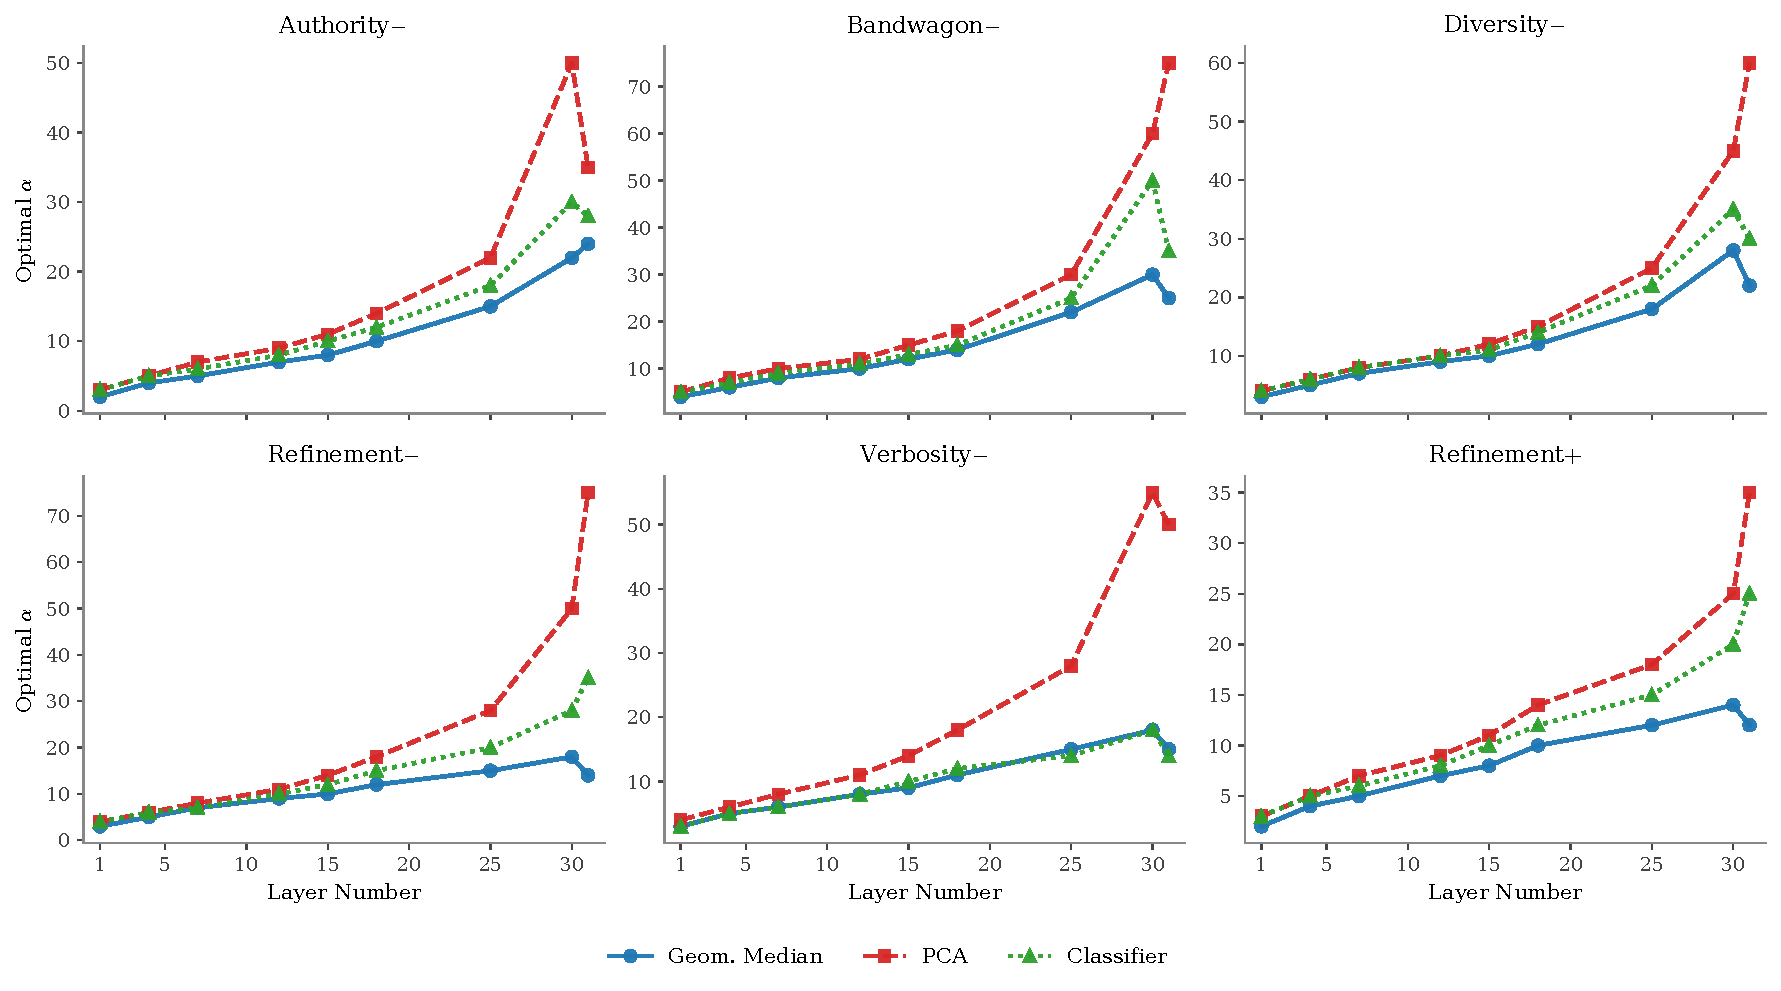
\includegraphics[width=\textwidth]{images/attack_alpha_per_bias.pdf}
\caption{Optimal intervention strength $\alpha^{*}$ as a function of layer for each of the six bias types, separately for the three vector methods (Geometric Median, PCA, Classifier). Layer indices are sampled at $\{1,4,7,12,15,18,25,30,31\}$. PCA consistently requires the largest strength at the late layers; all methods drop at layer 31 because the score-readout projection tightens the Spearman constraint.}
\label{fig:attack_alpha_per_bias}
\end{figure*}

\paragraph{Validity remains saturated.}
\Cref{fig:attack_success_heatmap} reports the output validity rate of the attack (fraction of perturbed inputs whose decoded score is still an integer in $\{1,\dots,10\}$) across all bias-layer combinations. Validity sits in $[0.96, 1.00]$ everywhere. The binding constraint on $\alpha^{*}$ is therefore the Spearman correlation, not generation integrity: the model still decodes a valid integer under strong activation steering, but the ordinal logic between answer quality and score breaks down before any malformed output appears.

\begin{figure*}[t]
\centering
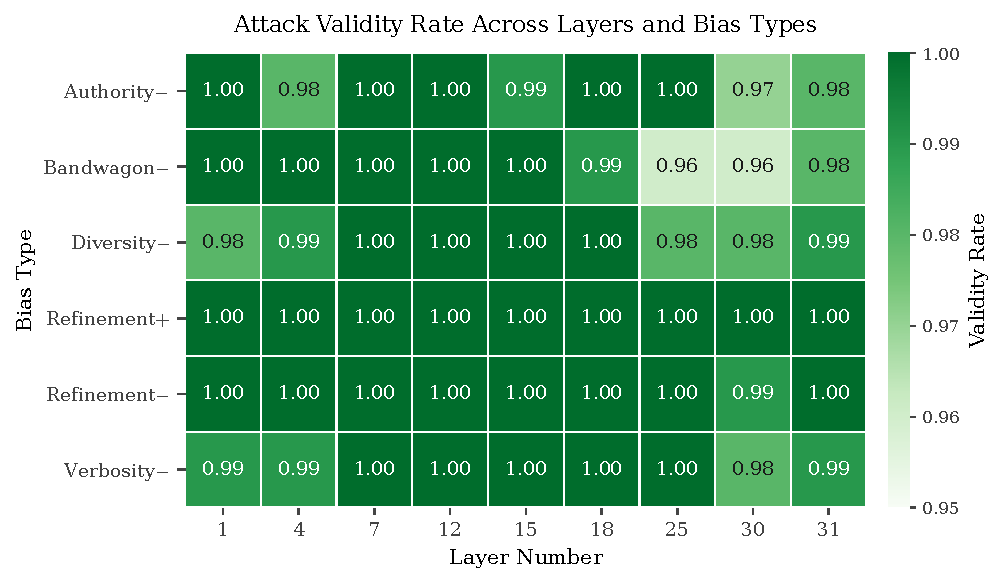
\includegraphics[width=0.85\textwidth]{images/attack_success_heatmap.pdf}
\caption{Output validity rate of the activation attack averaged over the three vector methods, for each (bias, layer) cell. All cells lie in $[0.96, 1.00]$: malformed decodes are not the binding constraint, the Spearman constraint is.}
\label{fig:attack_success_heatmap}
\end{figure*}

\paragraph{$\alpha^{*}$ and $W_1$ across the layer stack.}
\Cref{fig:attack_metrics_across_layers} summarizes the same data along the layer axis by averaging over methods. The top panel shows that all six biases share the same qualitative ``hockey-stick'' shape in $\alpha^{*}$, with Bandwagon$-$ requiring the largest strength at the late layers and Refinement$+$ the smallest. The bottom panel shows the corresponding score-shift: $W_1$ stays in $[0.4, 0.7]$ across the middle layers, then jumps at layer 31 for the strongest biases (Bandwagon$-$ to $1.75$). The narrow band of mid-layer $W_1$ confirms that the bias signal is broadly distributed in depth, not concentrated at a single ``critical'' layer.

\begin{figure*}[t]
\centering
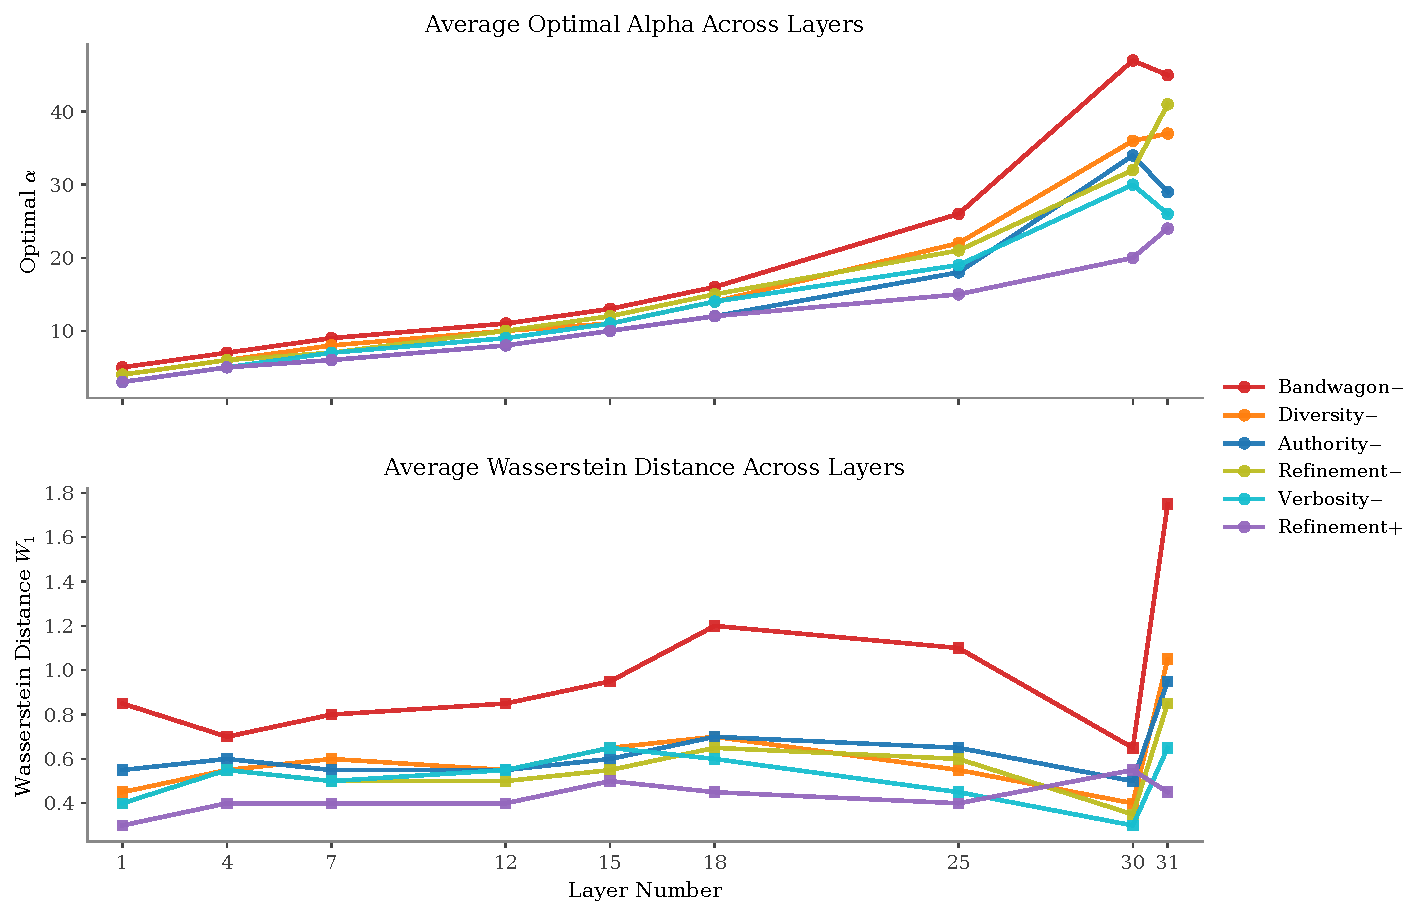
\includegraphics[width=\textwidth]{images/attack_metrics_across_layers.pdf}
\caption{Average optimal $\alpha$ (top) and average Wasserstein distance $W_1$ (bottom) across the layer stack, with one curve per bias type. Values are averaged over the three vector methods. All six biases share the same hockey-stick shape in $\alpha^{*}$, with the steepest climb at layers 30--31.}
\label{fig:attack_metrics_across_layers}
\end{figure*}

\paragraph{Method-level behavior.}
\Cref{fig:attack_metrics_by_method} averages instead over biases and separates the three vector methods. PCA needs the largest $\alpha$ but also produces the largest $W_1$, especially at the deep layers; Classifier vectors sit in the middle on both axes; Geometric Median is the gentlest, with the smallest $\alpha$, the smallest $W_1$, and the highest Spearman correlation. Together with the per-bias plots above, this is why we keep all three representatives in \Cref{subsec:causal}: the three methods sit at distinct points in the (strength, faithfulness) plane rather than along a single axis.

\begin{figure*}[t]
\centering
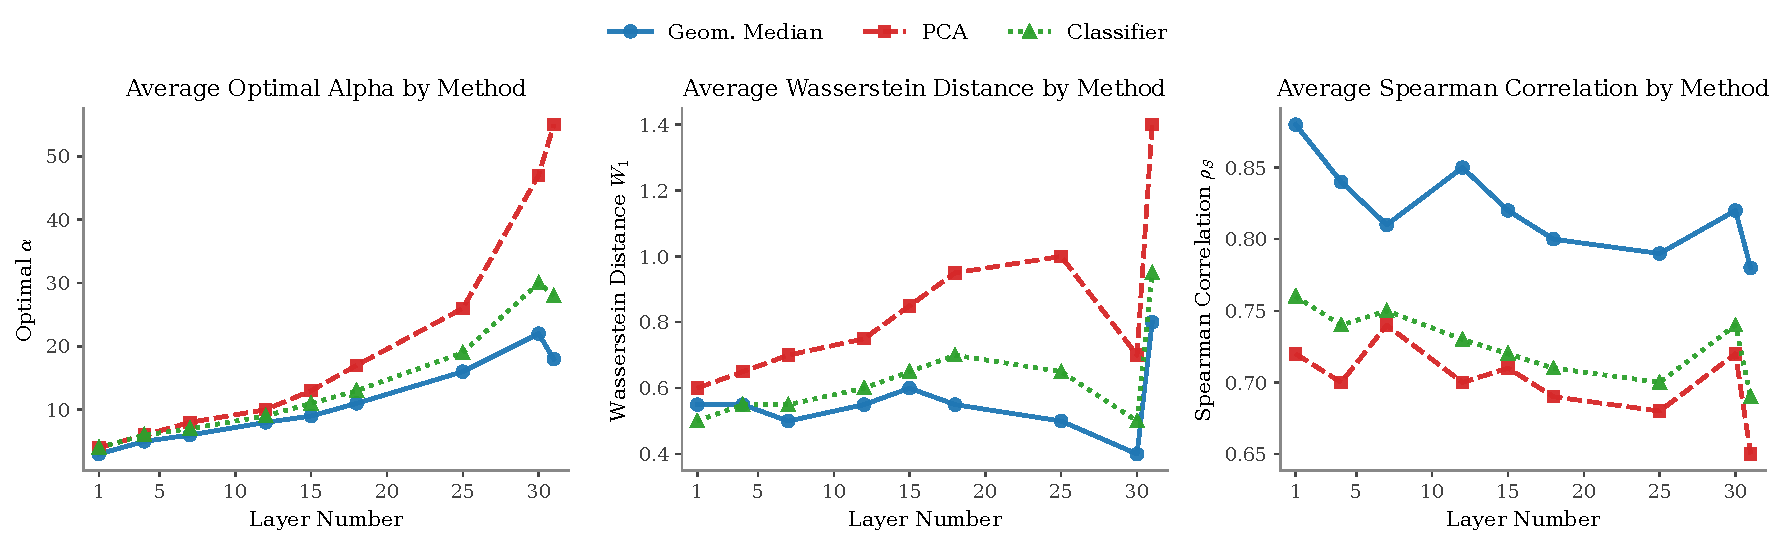
\includegraphics[width=\textwidth]{images/attack_metrics_by_method.pdf}
\caption{Average optimal $\alpha$, average Wasserstein distance $W_1$, and average Spearman correlation $\rho_S$ as a function of layer, separately for the three vector methods (averaged over the six bias types). PCA produces the strongest attacks at the cost of the lowest ordinal faithfulness; Geometric Median is the gentlest on both axes; Classifier sits in between.}
\label{fig:attack_metrics_by_method}
\end{figure*}


\section{Defense Results}
\label{app:defense_full}

Mirroring the attack setup, the defense applies $\vec{h}'_l = \vec{h}_l - \alpha\,\vec{v}_{\text{bias}}^{(l)}$ to inputs in $\mathcal{D}_{\text{eff}}^{-}$ (effective negative-bias samples), aiming to restore the unperturbed baseline score. Optimization reuses \Cref{alg:alpha_search} with the target score changed from baseline to biased, i.e.\ we maximize $W_1$-reduction
\begin{equation}
    \Delta W_1^{\text{def}}(\alpha) \;=\; 1 \;-\; \frac{W_1\!\left(s(\vec{h}'_l(\alpha)),\, s(\vec{h}_l^{\text{base}})\right)}{W_1\!\left(s(\vec{h}_l),\, s(\vec{h}_l^{\text{base}})\right)},
\end{equation}
subject to the same validity ($\geq 95\%$) and Spearman ($\geq 1.1\rho_S^{\text{text-rewrite}}$) constraints. The text-rewrite baseline paraphrases the perturbed answer with a neutralization prompt (\eg, for Bandwagon$-$ it asks an LLM to strip the consensus attribution while preserving the answer body), emulating the obvious text-level counterpart.

\begin{table*}[h!]
\centering
\small
\setlength{\tabcolsep}{6pt}
\caption{Complete defense performance on \textsc{Llama-3.1-8B}, test set. Each block shows the best per-method configuration selected on the development set; the evaluation metric is the fractional reduction in $W_1$ between defended and original baseline score distributions.}
\label{tab:defense_full}
\begin{tabular}{l l c c c c c}
\toprule
\textbf{Bias} & \textbf{Method} & $\Delta W_1^{\text{def}} \uparrow$ & $\rho_S \uparrow$ & \textbf{Valid.} & \textbf{Layer} & $|\alpha^{*}|$ \\
\midrule
\multirow{4}{*}{Authority$-$} & Text Rewrite & 0.11 & 0.74 & 100\% & -- & -- \\
 & Geometric Median & 0.49 & \textbf{0.84} & 99.0\% & 25 & 18.3 \\
 & PCA & 0.56 & 0.79 & 96.8\% & 27 & 31.2 \\
 & \textbf{Classifier} & \textbf{0.62} & 0.81 & 96.5\% & 28 & 54.7 \\
\midrule
\multirow{4}{*}{Bandwagon$-$} & Text Rewrite & 0.09 & 0.56 & 100\% & -- & -- \\
 & Geometric Median & 0.47 & \textbf{0.71} & 98.5\% & 22 & 9.6 \\
 & \textbf{PCA} & \textbf{0.61} & 0.67 & 95.9\% & 29 & 48.2 \\
 & Classifier & 0.56 & 0.65 & 96.2\% & 23 & 12.4 \\
\midrule
\multirow{4}{*}{Refinement$-$} & Text Rewrite & 0.15 & 0.77 & 100\% & -- & -- \\
 & Geometric Median & 0.41 & \textbf{0.86} & 100\% & 20 & 3.9 \\
 & PCA & 0.48 & 0.83 & 98.6\% & 29 & 21.8 \\
 & \textbf{Classifier} & \textbf{0.52} & 0.83 & 97.1\% & 24 & 6.5 \\
\bottomrule
\end{tabular}
\end{table*}

Defense results mirror the attack findings in structure: activation-based defense dominates the text-rewrite baseline by a factor of 3--5$\times$ in $W_1$-reduction across all three bias types, while simultaneously maintaining comparable or higher Spearman correlation. The optimal defense layer tends to be slightly shallower than the optimal attack layer (20--29 vs.\ 18--31), consistent with the intuition that reaching the fair region from a biased state requires intervention before the late-layer reorganization finalizes the scoring decision. Geometric Median defenses again produce the most rank-preserving results, while Classifier defenses yield the largest $W_1$-reductions on two of three bias types. Critically, the symmetry between effective attack and effective defense along the \emph{same} vector $\vec{v}_{\text{bias}}^{(l)}$ is the core causal claim of \Cref{subsec:causal}: the bias direction admits bidirectional steering.

\section{Additional Activation Visualizations}
\label{app:visualizations}

The layer-25 fair-region projection (\Cref{fig:activation_mds_combined}) appears in the main text; this appendix gathers additional projections that support the geometric claims of \Cref{subsec:geometry}.

\subsection{Activation MDS Across Layers}

\Cref{fig:activation_mds_layers} presents MDS projections of absolute activations at layers 5, 15, and 25 of \textsc{Llama-3.1-8B}. The same pattern holds across all layers: baseline activations form a tight cluster, while most negatively biased activations are displaced to a distant region, with a small subset remaining anomalously close to the baseline.

\begin{figure*}[t]
\centering
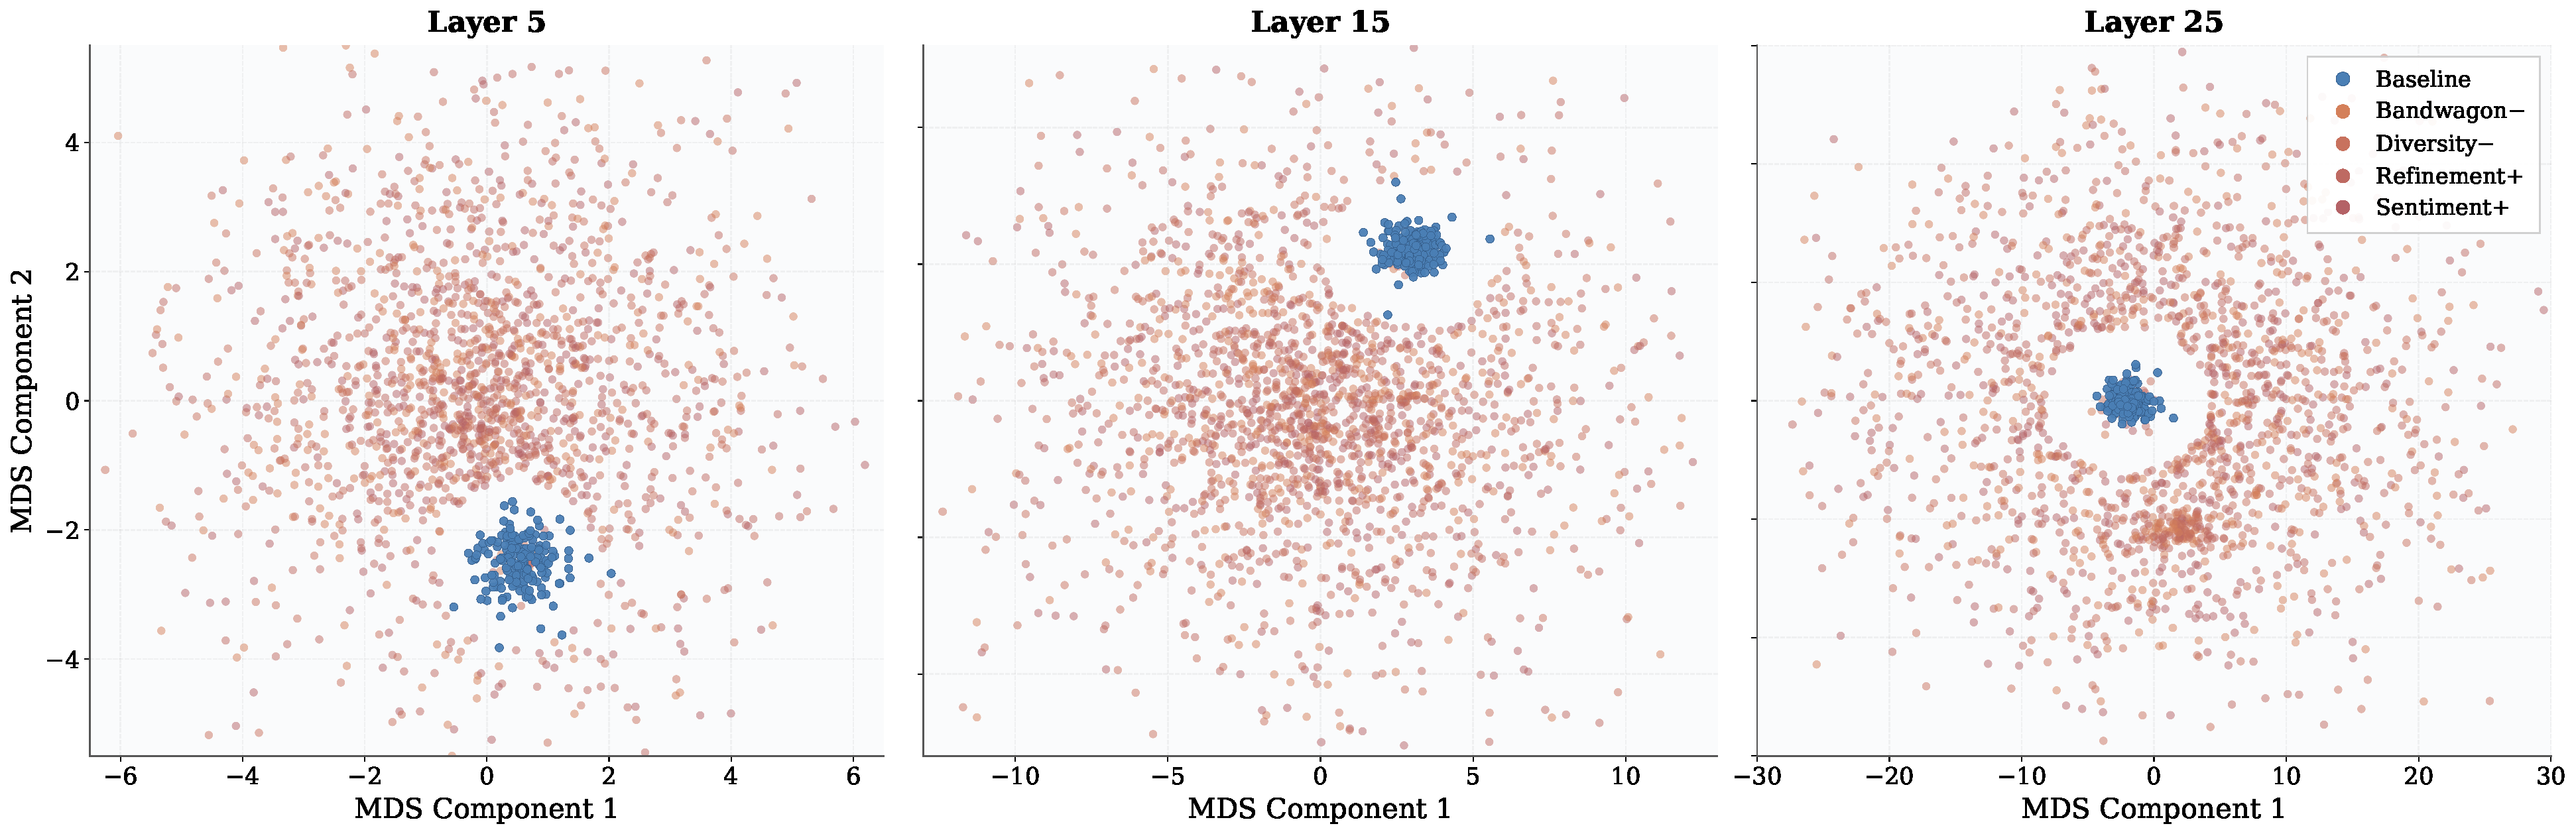
\includegraphics[width=\textwidth]{images/activation_mds_layers_combined.pdf}
\caption{MDS projection of final-token activations at layers 5, 15, and 25 of \textsc{Llama-3.1-8B} for $\mathcal{D}_{\text{base}}$ and $\mathcal{D}_{\text{neg}}$. The clustering pattern---tight baseline region with displaced biased activations---is consistent across layers.}
\label{fig:activation_mds_layers}
\end{figure*}

\subsection{Same-Polarity Geometric Separation}

\Cref{fig:mds_neg_neg} presents MDS projections of per-sample effective bias vectors $\Delta \vec{h}_l$ for two \emph{negative} bias types---Bandwagon and Diversity---at layers 5, 15, and 25. As with the cross-polarity comparison (\Cref{fig:mds_bias_vectors}), the two negative types become increasingly separable in deeper layers, confirming that geometric distinction is a general property of bias-type representations, not an artifact of polarity differences.

\begin{figure*}[t]
\centering
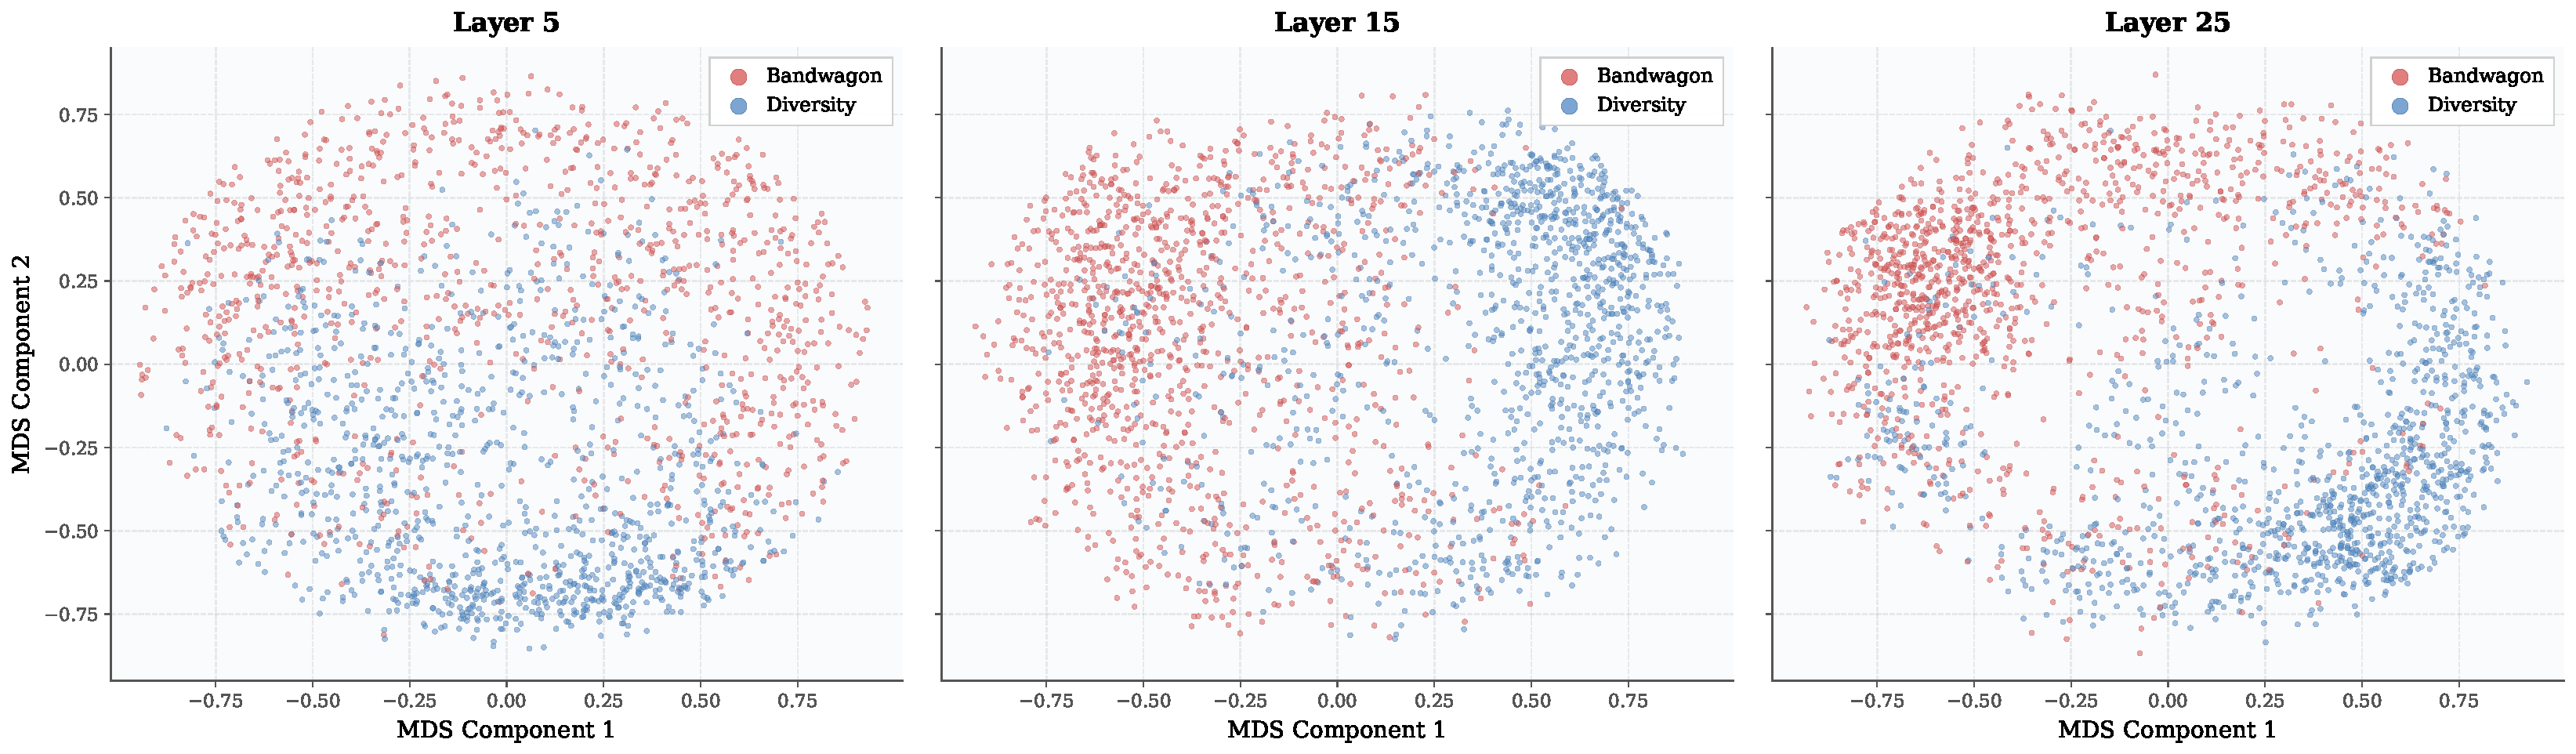
\includegraphics[width=\textwidth]{images/effective_bias_vectors_3layers.pdf}
\caption{MDS projection of per-sample effective bias vectors $\Delta \vec{h}_l$ for Bandwagon (red) and Diversity (blue) negative biases at layers 5, 15, and 25 of \textsc{Llama-3.1-8B}. The two negative bias types exhibit progressive geometric separation in deeper layers.}
\label{fig:mds_neg_neg}
\end{figure*}

\subsection{Layer-wise Direction Concentration}
\label{app:layerwise_table}

\Cref{tab:layerwise} reports the four scalars summarized in \Cref{subsec:layer_analysis} at six representative layers of \textsc{Llama-3.1-8B}: the biased-core fraction $\rho_{\text{core}}^{(l)}$, the LDA separability $\text{Sep}_{\text{LDA}}^{(l)}$, the raw classifier AUC, and the cosine agreement between the LDA and Classifier direction estimates. Biased-core fraction and LDA separability rise monotonically with depth; cosine agreement climbs from $0.52$ at layer~5 to $0.94$ at layer~31, indicating that two estimators with entirely different objectives converge on the same axis at late layers; raw classifier AUC peaks in middle layers, where surface-cue separability is still trivially exploitable.

\begin{table}[t]
\centering
\small
\setlength{\tabcolsep}{3pt}
\caption{Layer-wise characterization of the bias direction on \textsc{Llama-3.1-8B} (32 layers). Biased core $\rho_{\text{core}}$, LDA separability, and the LDA/Classifier cosine agreement rise monotonically with depth; raw classifier AUC peaks in middle layers.}
\label{tab:layerwise}
\begin{tabular}{c cccc}
\toprule
$l$ & $\rho_{\text{core}}^{(l)}$ & $\text{Sep}_{\text{LDA}}^{(l)}$ & AUC$_{\text{CLS}}$ & $\cos(\vec{v}_{\text{LDA}}, \vec{v}_{\text{CLS}})$ \\
\midrule
\phantom{0}5 & 0.32 & 0.71 & 0.89 & 0.52 \\
10 & 0.48 & 0.79 & \textbf{0.94} & 0.68 \\
15 & 0.62 & 0.85 & \textbf{0.94} & 0.78 \\
20 & 0.73 & 0.90 & 0.93 & 0.85 \\
25 & 0.81 & 0.93 & 0.91 & 0.91 \\
31 & \textbf{0.87} & \textbf{0.95} & 0.87 & \textbf{0.94} \\
\bottomrule
\end{tabular}
\end{table}

\subsection{Magnitude Consistency Across Layers}
\label{app:l2_norm}

\Cref{fig:l2_norm} plots the per-layer mean L2 norm of final-token activations for $\mathcal{D}_{\text{base}}$ and $\mathcal{D}_{\text{neg}}$ on \textsc{Llama-3.1-8B}. The two trajectories are statistically indistinguishable at every layer, with the maximum relative gap (3.5\%) concentrated at the final score-readout layer where the linear head projects the activation onto the score logits. Everywhere else the gap sits below 2\%. Bias is therefore encoded in the \emph{direction} of the activation displacement rather than in its magnitude. This is why we unit-normalize the vector estimators throughout \Cref{subsec:bias_direction,subsec:causal}, and why we define the biased core in terms of Mahalanobis distance, as in \Cref{tab:layerwise}.

\begin{figure}[t]
\centering
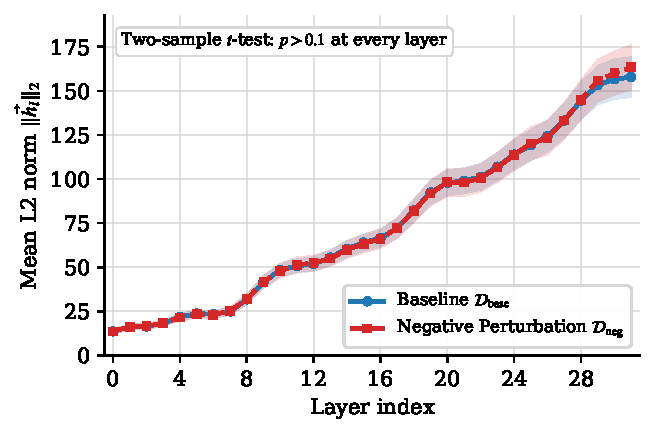
\includegraphics[width=\columnwidth]{images/l2_norm_layers.pdf}
\caption{Mean L2 norm of final-token activations across the 32 decoder layers of \textsc{Llama-3.1-8B} for the baseline set $\mathcal{D}_{\text{base}}$ (blue, solid) and the negatively perturbed set $\mathcal{D}_{\text{neg}}$ (red, dashed). Shaded bands denote $\pm 1$ SD across samples. Bias does not change how far the activation moves; only the direction in which it moves.}
\label{fig:l2_norm}
\end{figure}

\subsection{PCA Analysis of Activation Space}

\begin{wrapfigure}{r}{0.48\columnwidth}
\vspace{-1em}
\centering
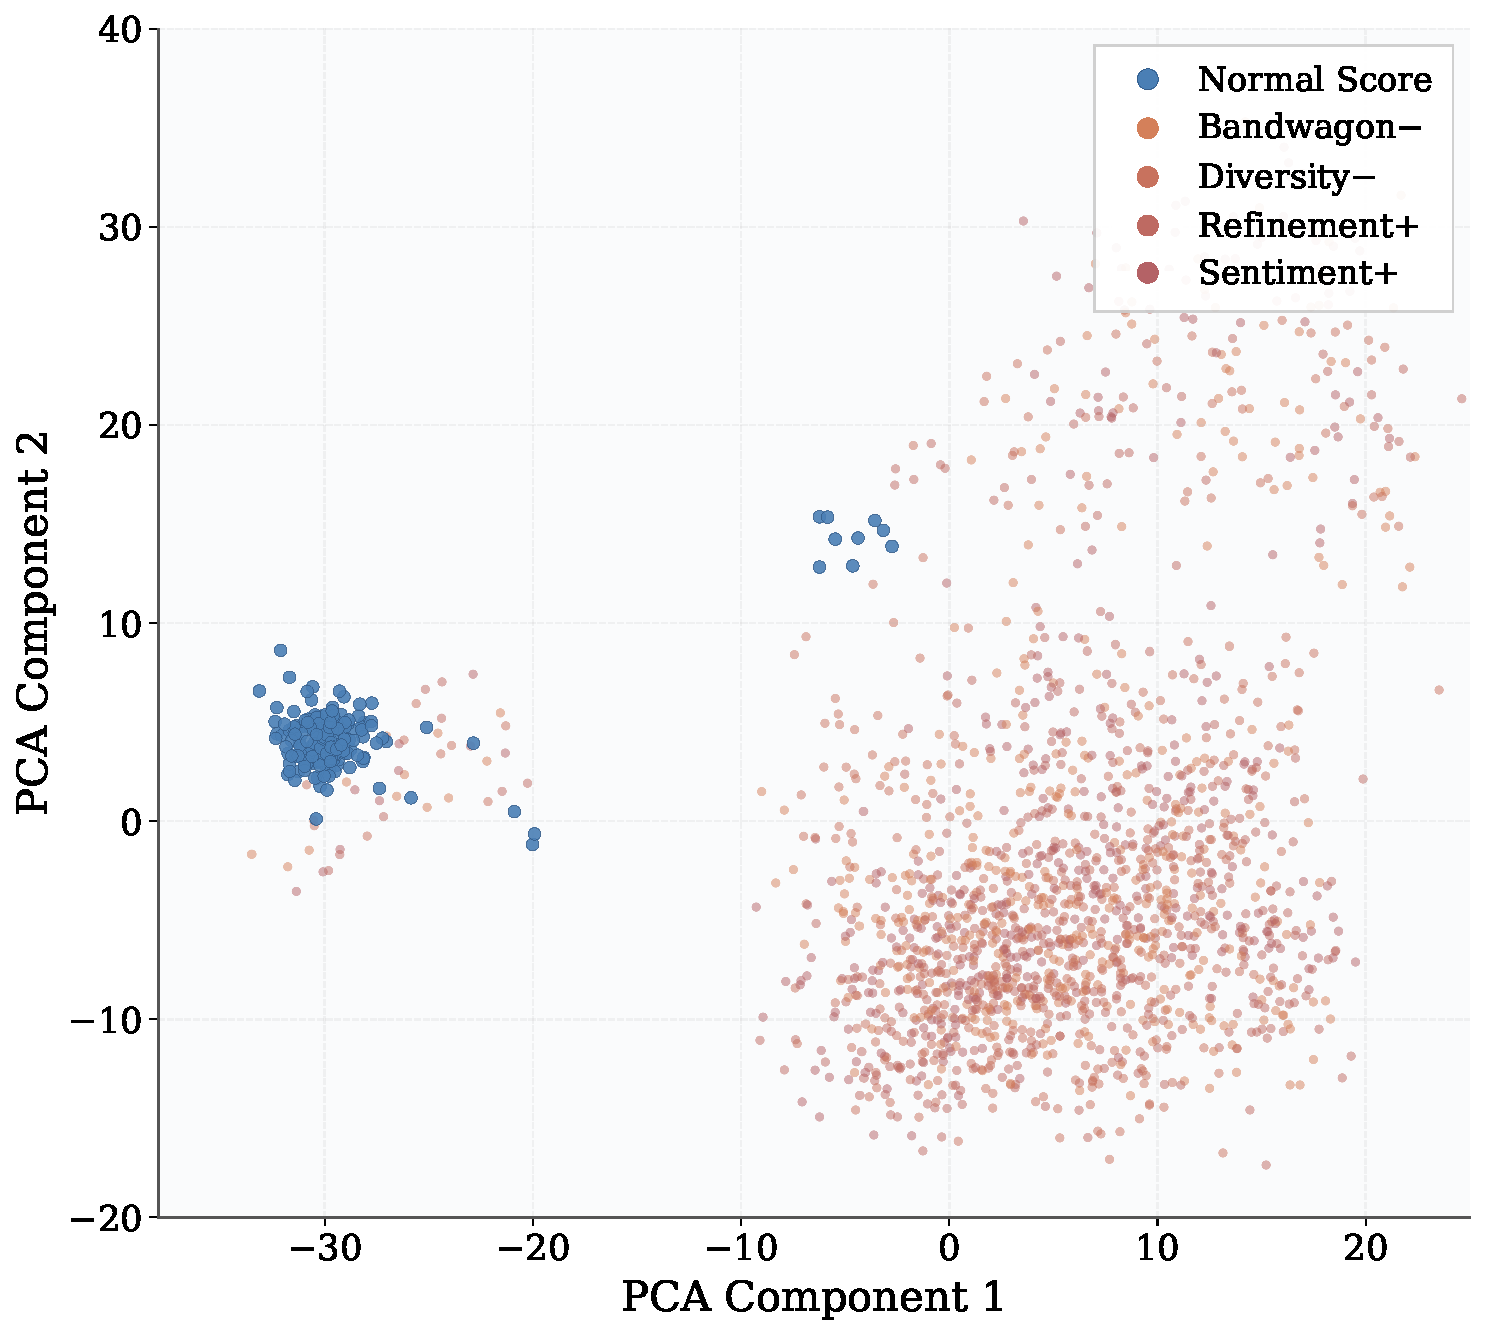
\includegraphics[width=0.47\columnwidth]{images/pca_activation.pdf}
\caption{PCA projection of final-token activations at layer 25 of \textsc{Llama-3.1-8B}, colored by bias type. Baseline activations cluster tightly into a fair zone, mirroring the MDS visualization in the main text.}
\label{fig:pca_appendix}
\vspace{-1em}
\end{wrapfigure}

\Cref{fig:pca_appendix} shows a PCA projection of final-token activations at layer 25 of \textsc{Llama-3.1-8B}, colored by bias type. Consistent with the MDS analysis (\Cref{fig:activation_mds_combined}), baseline activations form a tight cluster---the fair zone---while effective bias samples from different bias types are displaced away from this region. The agreement between MDS and PCA confirms that the fair zone is a robust geometric property of the activation space, not an artifact of a particular dimensionality reduction method.

\section{Detection Pipeline Details}
\label{app:detection_details}

This appendix provides the full details behind the detection results summarized in \Cref{subsec:detection_brief}, including feature construction, training protocol, baseline comparisons, and a domain-gap diagnostic.

\subsection{Feature Construction and Training Protocol}

For each input $x$, we compute a per-layer feature vector $\vec{\phi}_l(x)$ drawn from three families, then concatenate across layers:
\begin{itemize}[leftmargin=1.2em, nosep]
    \item \textbf{Bias-direction features}: the scalar projection $\vec{h}_l(x)^{\top} \vec{v}_{\text{LDA}}^{(l)}$, the scalar projection $\vec{h}_l(x)^{\top} \vec{v}_{\text{CLS}}^{(l)}$, cosine similarities $\cos(\vec{h}_l(x) - \vec{\mu}_{\text{base}}^{(l)},\, \vec{v}_{\cdot}^{(l)})$, and the perpendicular distance $\|(\vec{h}_l(x) - \vec{\mu}_{\text{base}}^{(l)}) - \text{proj}_{\vec{v}_{\cdot}^{(l)}}(\cdot)\|_2$ for both vector types.
    \item \textbf{Manifold-deviation features}: the Mahalanobis distance $d_M(\vec{h}_l(x); \vec{\mu}_{\text{base}}^{(l)}, \vec{\Sigma}_{\text{base}}^{(l)})$ and its $z$-score against the baseline distribution.
    \item \textbf{Semantic-context features}: the top-$k$ PCA projections of $\vec{h}_l(x)$ onto the baseline PCA basis, and intrinsic statistics ($\|\vec{h}_l(x)\|_2$, mean, variance of the activation).
\end{itemize}
Per layer this yields $K \approx 14$ features, and concatenated across $L=32$ layers we obtain a $\sim 450$-dimensional representation. Recursive Feature Elimination (RFE) prunes this to roughly 120 features, and a Gradient Boosting Decision Tree (GBDT, LightGBM) is trained with 200 rounds of Bayesian hyperparameter search (Optuna) against the development AUC. The detection target is the scoring outcome (\Cref{subsec:detection_method}), not a stylistic classification.

\subsection{Baseline Detectors}

We compare against four baselines that span two families: (i) linear baselines using subsets of the same activation features, and (ii) text-based detectors that ignore activations entirely.

\begin{table*}[h!]
\centering
\small
\setlength{\tabcolsep}{6pt}
\caption{Bias-detection performance on \textsc{Llama-3.1-8B}. The test set contains three benchmarks unseen during training, exposing a genuine domain gap. The GBDT detector matches or outperforms all baselines on AP and is competitive on AUC, despite markedly higher development-set AUC indicating room for further domain adaptation.}
\label{tab:detection_baselines}
\begin{tabular}{l cc cc}
\toprule
& \multicolumn{2}{c}{\textbf{Dev (in-domain)}} & \multicolumn{2}{c}{\textbf{Test (incl.\ unseen)}} \\
\cmidrule(lr){2-3} \cmidrule(lr){4-5}
\textbf{Detector} & AUC & AP & AUC & AP \\
\midrule
Text-based LLM Detector & 0.641 & 0.939 & 0.633 & 0.937 \\
PCA + Logistic Regression & 0.871 & 0.971 & 0.837 & 0.969 \\
Projection + Mahalanobis (linear) & 0.864 & 0.974 & 0.834 & 0.972 \\
Projection Features Only (linear) & 0.883 & 0.979 & \textbf{0.854} & 0.977 \\
\midrule
\textbf{GBDT (ours)} & \textbf{0.926} & \textbf{0.992} & 0.839 & \textbf{0.976} \\
\bottomrule
\end{tabular}
\end{table*}

Three observations warrant note. First, the text-based LLM detector substantially underperforms every activation-based approach, echoing our main-text claim that the bias signal is much cleaner in the activation geometry than in the input text. Second, the linear baselines perform surprisingly well---Projection Features Only attains test AUC 0.854---confirming that the bias direction is itself highly informative. Third, the GBDT opens a visible gap on the development set (0.926 vs.\ 0.883 AUC) but loses most of it on the cross-domain test set (0.839 vs.\ 0.854). This gap is the principal weakness of the detector in its current form.

\subsection{Component Ablations}
\label{app:detection_ablation}

The cross-method comparison above shows that the GBDT is competitive with simpler activation-based baselines but does not dominate them on the cross-domain test set. To isolate which parts of the pipeline are actually doing the work---and to argue that the 0.84 test AUC is closer to a ceiling than a floor for this feature set---we run a component-level ablation that varies the GBDT inputs and the pipeline itself. Each row keeps the LightGBM model, Bayesian hyperparameter search, and class-balanced training identical; only the feature set or the feature-selection step changes.

\begin{table*}[h!]
\centering
\small
\setlength{\tabcolsep}{6pt}
\caption{GBDT detection performance as a function of feature subset and pipeline component on \textsc{Llama-3.1-8B}. Each row uses the same LightGBM model and the same Optuna search budget; the feature set or the feature-selection step is the only thing that changes between rows. Best in column in bold.}
\label{tab:detection_ablation}
\begin{tabular}{l cc cc}
\toprule
& \multicolumn{2}{c}{\textbf{Dev (in-domain)}} & \multicolumn{2}{c}{\textbf{Test (incl.\ unseen)}} \\
\cmidrule(lr){2-3} \cmidrule(lr){4-5}
\textbf{GBDT variant} & AUC & AP & AUC & AP \\
\midrule
Mahalanobis distance only (1 feat.) & 0.768 & 0.957 & 0.711 & 0.949 \\
PCA / intrinsic-statistic features only (57 feat.) & 0.872 & 0.974 & 0.792 & 0.961 \\
Bias-direction projections only (41 feat.) & 0.918 & 0.989 & 0.831 & 0.973 \\
All features, no RFE ($\sim 450$ feat., raw) & 0.918 & 0.988 & 0.825 & 0.971 \\
\textbf{All features + RFE + Optuna (ours)} & \textbf{0.926} & \textbf{0.992} & \textbf{0.839} & \textbf{0.976} \\
\bottomrule
\end{tabular}
\end{table*}

Three things stand out. First, Mahalanobis distance on its own---essentially asking ``does this activation look like it came from the fair zone?''---already achieves test AUC 0.71, well above the 0.63 of the text-based LLM baseline; geometry alone, even reduced to a single scalar, beats the most natural prompted detector. Second, the bias-direction projections alone (the cosine and signed projection onto $\vec{v}_{\text{LDA}}^{(l)}$ and $\vec{v}_{\text{CLS}}^{(l)}$ at each layer) reach test AUC 0.831, within 1 point of the full pipeline; the bias direction is doing roughly 95\% of the heavy lifting on the cross-domain test set, consistent with the 62.3\% Gini importance it carries in the final model (\Cref{tab:detection_feature_importance}). Third, RFE buys only a modest gain on the test set (0.825 $\to$ 0.839 AUC) but reduces the dev--test gap from 0.093 to 0.087: most of the residual gap is irreducible under this feature set rather than a symptom of an oversized feature pool. Taken together, these numbers position 0.84 as the ceiling of what bias-geometric features yield for cross-domain detection on this judge, not as the floor of an under-engineered model---and motivate the domain-gap diagnostic below.

\subsection{Domain-Gap Diagnostic}

To quantify the cross-domain generalization shortfall, we evaluate the GBDT separately on the test-set questions drawn from the six \emph{seen} benchmarks versus those drawn from the three \emph{unseen} benchmarks.

\begin{table*}[h!]
\centering
\small
\setlength{\tabcolsep}{6pt}
\caption{GBDT detection performance on test-set splits conditioned on whether the source benchmark was present in training.}
\label{tab:detection_domain}
\begin{tabular}{l cc cc}
\toprule
& \multicolumn{2}{c}{\textbf{Seen benchmarks}} & \multicolumn{2}{c}{\textbf{Unseen benchmarks}} \\
\cmidrule(lr){2-3} \cmidrule(lr){4-5}
\textbf{Detector} & AUC & AP & AUC & AP \\
\midrule
Text-based LLM Detector & 0.638 & 0.942 & 0.624 & 0.928 \\
Projection Features Only & 0.869 & 0.981 & 0.821 & 0.967 \\
\textbf{GBDT (ours)} & \textbf{0.902} & \textbf{0.988} & 0.751 & 0.953 \\
\bottomrule
\end{tabular}
\end{table*}

Within-domain, the GBDT attains AUC 0.902, close to its development performance. On held-out benchmarks, AUC drops to 0.751---still well above the text-based baseline (0.624), but well below the within-domain figure. The linear Projection Features detector is more robust to the domain shift but leaves performance on the table within domain. This suggests that the GBDT is overfitting to domain-specific activation patterns rather than fully exploiting the universal bias-direction signal, and motivates future work on domain-adversarial training or feature regularization targeting the bias subspace identified in \Cref{subsec:layer_analysis}.

\subsection{Feature Importance}

\Cref{tab:detection_feature_importance} groups the RFE-retained features by family and reports their mean Gini importance in the final GBDT. Bias-direction projections alone account for over 60\% of the total importance, consistent with the main-text claim that $\vec{v}_{\text{LDA}}$ and $\vec{v}_{\text{CLS}}$ capture the dominant bias signal. Among individual layers, layers 22--28 contribute disproportionately, matching the layer-wise sweet spot identified in \Cref{tab:layerwise}.

\begin{table*}[h!]
\centering
\small
\setlength{\tabcolsep}{6pt}
\caption{Feature-family importance in the GBDT detector (Gini importance, normalized to sum to 100\%).}
\label{tab:detection_feature_importance}
\begin{tabular}{l c c}
\toprule
\textbf{Feature Family} & \textbf{\# features retained} & \textbf{Gini importance} \\
\midrule
Bias-direction projections ($\vec{v}_{\text{LDA}}, \vec{v}_{\text{CLS}}$) & 41 & 62.3\% \\
Mahalanobis distance from $\mathcal{M}_{\text{fair}}$ & 22 & 18.7\% \\
PCA / intrinsic-statistic features & 57 & 19.0\% \\
\bottomrule
\end{tabular}
\end{table*}


\end{document}
